%-------------------------------------------------------------------------------
%	REQUIRED PACKAGES AND  CONFIGURATIONS
%-------------------------------------------------------------------------------

%\documentclass[temporary]{oist_thesis} % Temporary version for thesis revision and examination
\documentclass[final]{oist_thesis} % Final version for thesis submission

% To show \subsubsection{} numbered in TOC
\setcounter{tocdepth}{2}
\setcounter{secnumdepth}{2}

\usepackage[english]{babel} % The document is in English
\usepackage[utf8]{inputenc} % UTF8 encoding
\usepackage[T1]{fontenc} % Font encoding

\usepackage{graphicx} % For including images
\graphicspath{{./Images/}} % Specifies the directory where pictures are stored

\usepackage{eso-pic} % For the background picture on the title page

\usepackage{setspace} % For using single or double spacing
\usepackage{longtable} % tables that can span several pages
\usepackage{pdfpages} % To include a pdf files of your published papers as an appendix
\usepackage{fancyhdr} % For the headers
\usepackage{hyperref} % Adds clickable links at references
\usepackage{afterpage} % blank page
\usepackage{bm}
\newcommand\blankpage{%
    \null
    \thispagestyle{empty}%
    \addtocounter{page}{0}%
    \newpage}
    
\newcommand\blankpageNN{%
    \null
    \thispagestyle{empty}%
    \addtocounter{page}{-1}%
    \newpage}
  

%-------------------------------------------------------------------------------
%	ADD YOUR PACKAGES (be careful of package interaction)
%-------------------------------------------------------------------------------

\usepackage{xcolor}
\usepackage{amsthm,amsmath,amssymb,amsfonts,bbm}% Math symbols

% Redefine the plain page style
\fancypagestyle{plain}{%
  \fancyhf{}%
  \fancyfoot[C]{\thepage}%
  \renewcommand{\headrulewidth}{0pt}% Line at the header invisible
  \renewcommand{\footrulewidth}{0.4pt}% Line at the footer visible
}

\usepackage{hyperref}
\usepackage{pdfpages}
\usepackage{dirtree}
\usepackage{amsmath}
\usepackage{cancel}
\usepackage{siunitx}
\usepackage{floatrow}
\usepackage{comment}
\usepackage{multirow}
\usepackage[colorinlistoftodos]{todonotes}
\usepackage{textcomp}
\usepackage{gensymb}
\usepackage{makecell}
\hypersetup{
    colorlinks,
    linkcolor={black!100!black},
    citecolor={black!100!black},
    urlcolor={black!100!black}
}
\usepackage[verbose]{placeins}
\usepackage{ragged2e}
\usepackage{nccmath}
\usepackage[absolute,overlay]{textpos}
\usepackage{titlesec}
\usepackage[version=4]{mhchem}
\usepackage[notransparent]{svg}
\usepackage{csquotes}


%-------------------------------------------------------------------------------
%	PDF METADATA
%-------------------------------------------------------------------------------

\hypersetup{
    pdfauthor={Luca Ghislotti},
    pdftitle={Characterisation of the readout electronics of the Si(Li) tracker for the first flight of the GAPS experiment},
    pdfsubject={This thesis work describes the characterisation work that has been carried out on the flight items of the lithium-drifted silicon tracker of the GAPS experiment and includes an in-depth description of the validation techniques used for all detector components and the results obtained during the testing process.},
    pdfkeywords={GAPS, Dark Matter, ASIC, Microelectronics},
    pdfproducer={Overleaf},
    pdfcreator={PdfTeX}
}


%-------------------------------------------------------------------------------
%	ADD YOUR DEFINITIONS AND COMMANDS
%-------------------------------------------------------------------------------

\makeatletter
\def\smallunderbrace#1{\mathop{\vtop{\m@th\ialign{##\crcr
   $\hfil\displaystyle{#1}\hfil$\crcr
   \noalign{\kern3\p@\nointerlineskip}%
   \tiny\upbracefill\crcr\noalign{\kern3\p@}}}}\limits}
\makeatother

\newfloatcommand{capbtabbox}{table}[][\FBwidth]
\renewcommand\labelitemi{$\vcenter{\hbox{\tiny$\bullet$}}$}

\newcommand\T{\rule{0pt}{2.6ex}}       % Top strut
\newcommand\B{\rule[-1.2ex]{0pt}{0pt}} % Bottom strut
\newcommand{\minus}{\scalebox{0.75}[1.5]{$-$}}
\sisetup{detect-weight=true, detect-family=true}


%-------------------------------------------------------------------------------
%	BIBLIOGRAPHY STYLE
%-------------------------------------------------------------------------------

\usepackage[
    backend=biber,
    style=numeric,
    sorting=none,
    maxnames=8,
]{biblatex}

\addbibresource{thesis_bibliography.bib}
\appto{\bibsetup}{\sloppy}
\AtEveryBibitem{
    \clearfield{urlyear}
    \clearfield{urlmonth}
}


%-------------------------------------------------------------------------------
%	TITLE PAGE
%-------------------------------------------------------------------------------

\begin{document}

\thispagestyle{empty}
\begin{textblock*}{\textwidth}(2.98cm,1.5cm)
    \begin{center}
        \vskip0.5cm
        \includesvg[scale=0.75]{Images/unibg_logo_vector.svg}  
    \end{center}
\end{textblock*}

\begin{textblock*}{\textwidth}(2.98cm,7cm)
    \begin{center}
        \large
        UNIVERSITY OF BERGAMO
    \end{center}
    \begin{center}
        School of Engineering
    \end{center}
    \vspace{-0.65cm}
    \begin{center}
        Master Degree in Computer Engineering
    \end{center}
    \vspace{-0.65cm}
    \begin{center}
        Class N. LM-32 - Ingegneria Informatica
    \end{center}
    \vspace{1cm}
    \begin{center}
        \LARGE
        \textbf{Characterisation of the readout electronics of the Si(Li) tracker for the first flight of the GAPS experiment}
    \end{center}
    \vspace{10.5cm}
    \begin{center}
         ACADEMIC YEAR 2021 / 2022
    \end{center}
\end{textblock*}

\begin{textblock*}{\textwidth}(3.05cm,17.3cm) 
    Supervisor:
\end{textblock*}
\begin{textblock*}{\textwidth}(3.05cm,18cm)
    Prof. Massimo Manghisoni
\end{textblock*}

\begin{textblock*}{\textwidth}(3.05cm,19.5cm)
    Co-Supervisors:
\end{textblock*}
\begin{textblock*}{\textwidth}(3.05cm,20.2cm)
    Elisa Riceputi, Ph.D.
\end{textblock*}
\begin{textblock*}{\textwidth}(3.05cm,20.7cm) 
    Paolo Lazzaroni, Ms.C.
\end{textblock*}

\begin{textblock*}{\textwidth}(11.65cm,21.9cm)
    Master Thesis
\end{textblock*}
\begin{textblock*}{\textwidth}(11.65cm,22.6cm)
    Luca GHISLOTTI
\end{textblock*}
\begin{textblock*}{\textwidth}(11.65cm,23.3cm) 
    Student ID: 1052975
\end{textblock*}
\blankpage


%-------------------------------------------------------------------------------
%	PREAMBLE PAGES
%-------------------------------------------------------------------------------

\startpreamble
\frontmatter % Use roman page numbering style (i, ii, iii, iv...) for the preamble pages

\unnumberedchapter{Acknowledgment} % Acknowledgment
\chapter*{Acknowledgment} 

I am overwhelmed in all humbleness and gratefulness to acknowledge my depth to my advisor Prof. Massimo Manghisoni for the continuous support of my thesis work, for his patience, motivation, enthusiasm and immense knowledge. His guidance helped me in all the time of research and writing of this thesis. I could not have imagined having a better advisor and mentor for master thesis work.\\
I would also like to thank Elisa and Paolo for their encouragement, insightful comments and support during my entire stay in the electronics laboratory. \\
Finally, I wish to thank my parents Luisa and Bortolo for their unconditional trust, timely encouragement, and endless patience.
\cleardoublepage
\thispagestyle{empty} % Page style needs to be empty for this page

\vspace*{8cm} 

\hfill
%\begin{parbox}{0.6\textwidth}{
\begin{parbox}{0.7\textwidth}{
\begin{flushright}

%Research is to see what everybody else has seen and to think what nobody else has thought. \\ \vspace{0.3cm} \textit{Albert Szent-Gyorgyi}

If offered a seat on a rocket ship, don't ask what seat. Just get on. \\ \vspace{0.3cm} \textit{Christa McAuliffe, Challenger Astronaut}


\end{flushright}}
\end{parbox}





%-------------------------------------------------------------------------------
%	LIST OF CONTENTS/FIGURES/TABLES
%-------------------------------------------------------------------------------

\unnumberedchapter{Contents} % Contents
\tableofcontents % Write out the Table of Contents
\unnumberedchapter{List of Figures} % List of Figures
\listoffigures % Write out the List of Figures 
\unnumberedchapter{List of Tables} % List of Tables
\listoftables % Write out the List of Tables


%-------------------------------------------------------------------------------
%	THESIS MAIN TEXT
%-------------------------------------------------------------------------------

\addtocontents{toc}{\vspace{2em}} % Add a gap in the Contents, for aesthetics
\mainmatter % Begin numeric (1,2,3...) page numbering

\unnumberedchapter{Introduction} % Title of the unnumbered chapter % Introduction
\chapter*{Introduction}  % Name of the unnumbered section

\par
According to what is supported by some astrophysics theories, about 90\% of the mass of the universe is made by a hypothetical form of matter named Dark Matter and its discovery is one of the main scientific objectives of the 21st century in the field of physics research. Dark Matter is not directly observable, since, unlike normal matter, it does not emit electromagnetic radiation and only manifests itself through gravitational effects. 

\par
In this context, the General AntiParticle Spectrometer (GAPS) project stands as a modern approach to the indirect search of Dark Matter through the detection of cosmic antideuterium. The experiment is developed by an international collaboration that includes Japanese, US and Italian institutes, and it is funded by NASA, INFN, ASI, JAXA, and other research and academic institutions. The instrument relies on two detectors: a time-of-flight system, which tags candidate events for the detector to save and makes a precise velocity measurement, and a tracker system based on lithium-drifted silicon, Si(Li), detectors, which serves as the target and tracker for the initial cosmic-ray particle and its annihilation products. An Application Specific Integrated Circuit (ASIC) called \textit{SLIDER32} designed in a commercial \SI{180}{\nano\meter} CMOS technology is currently employed for the readout of the lithium-drifted silicon detectors and will be used for the first flight of the experiment scheduled for late 2023 from the the McMurdo station in Antarctica. The experimental characterisation of the ASIC is the focus of the thesis work discussed  in the following pages.

\par
The manuscript is organised as follows. \hyperref[ch1]{Chapter \ref{ch1}} describes the characterisation work that has been performed on the ASIC using a purposely built test board in order to carry out an analysis of the performance of the integrated circuit under varying temperature conditions. The measurements were performed to highlight the variations to which the transfer function, current reference, global threshold voltage and electronic noise are subjected.

\par
\hyperref[ch2]{Chapter \ref{ch2}} analyses the test and validation work that has been carried out on the flight components of the lithium-drifted silicon tracker of the GAPS experiment. The test procedures for each of the items and the results obtained are reported, detailing for each component the expected performance compared to that obtained during the test procedure.

\par
Lastly, \hyperref[ch3]{Chapter \ref{ch3}} reports the results obtained during the experimental demonstration of cosmic muon detection using a fully assembled Si(Li) tracker module, using the ArduSiPM cosmic ray and nuclear radiation detector as a trigger for the readout electronics. A full description of the setup used during the experiment and the results obtained are given in this Chapter.

\par
A detailed description of the GAPS experiment, its scientific aims in the context of physics research and the instrument on which it is based are provided in \hyperref[appendixGAPSintro]{Appendix \ref{appendixGAPSintro}}, with \hyperref[appendixGAPSdarkmatter]{Section \ref{appendixGAPSdarkmatter}} providing a brief introduction to Dark Matter. % Introduction (unnumbered)

\numberedchapter % Regular chapters following: input your chapters here

\chapter{Evaluation of temperature effects on ASIC performance} \label{ch1}

This Chapter describes the characterisation activity that has been carried out on the SLIDER32 ASIC, described in \hyperref[gapsTrackingSystem]{Appendix \ref{gapsTrackingSystem}}. Specifically, the measurements were taken with a purposely developed test board described in \hyperref[testboardsetup]{Section \ref{testboardsetup}} and were aimed at the evaluation of thermal effects on:

\begin{enumerate}
    %\bfseries
    \itemsep0em 
    \item Bandgap reference current.
    \item Channel input-output characteristic.
    \item Digital-to-Analog Converter (DAC) used to set the global threshold voltage.
\end{enumerate}

\par
The characterisation activity has also been focused on the evaluation of electronic noise performance of the readout channel in the form of Equivalent Noise Charge (ENC), measured at a temperature of \SI{-40}{\celsius}, that is, the temperature at which the readout electronics will work during the experiment \cite{re_2022_a}, therefore a precise evaluation of the noise contribution at this temperature is of fundamental importance.

%-------------------------------------------------------------------------------
%	Test setup description and characterisation process
%-------------------------------------------------------------------------------

\section[Test setup description and characterisation process]{Test setup description and characterisation\\ process} \label{testboardsetup}

The setup used for the temperature characterisation of the SLIDER32 ASIC has been designed in two variants, which only differ on one component, namely an Agilent 34461A digital multimeter in version \texttt{1}, shown in \hyperref[figTESTBOARDsetup1]{Figure \ref{figTESTBOARDsetup1}}, in place of a Keysight E3631A DC power supply in version \texttt{2}, shown in \hyperref[figTESTBOARDsetup2]{Figure \ref{figTESTBOARDsetup2}}.

\begin{figure}[h!]
    \centering
    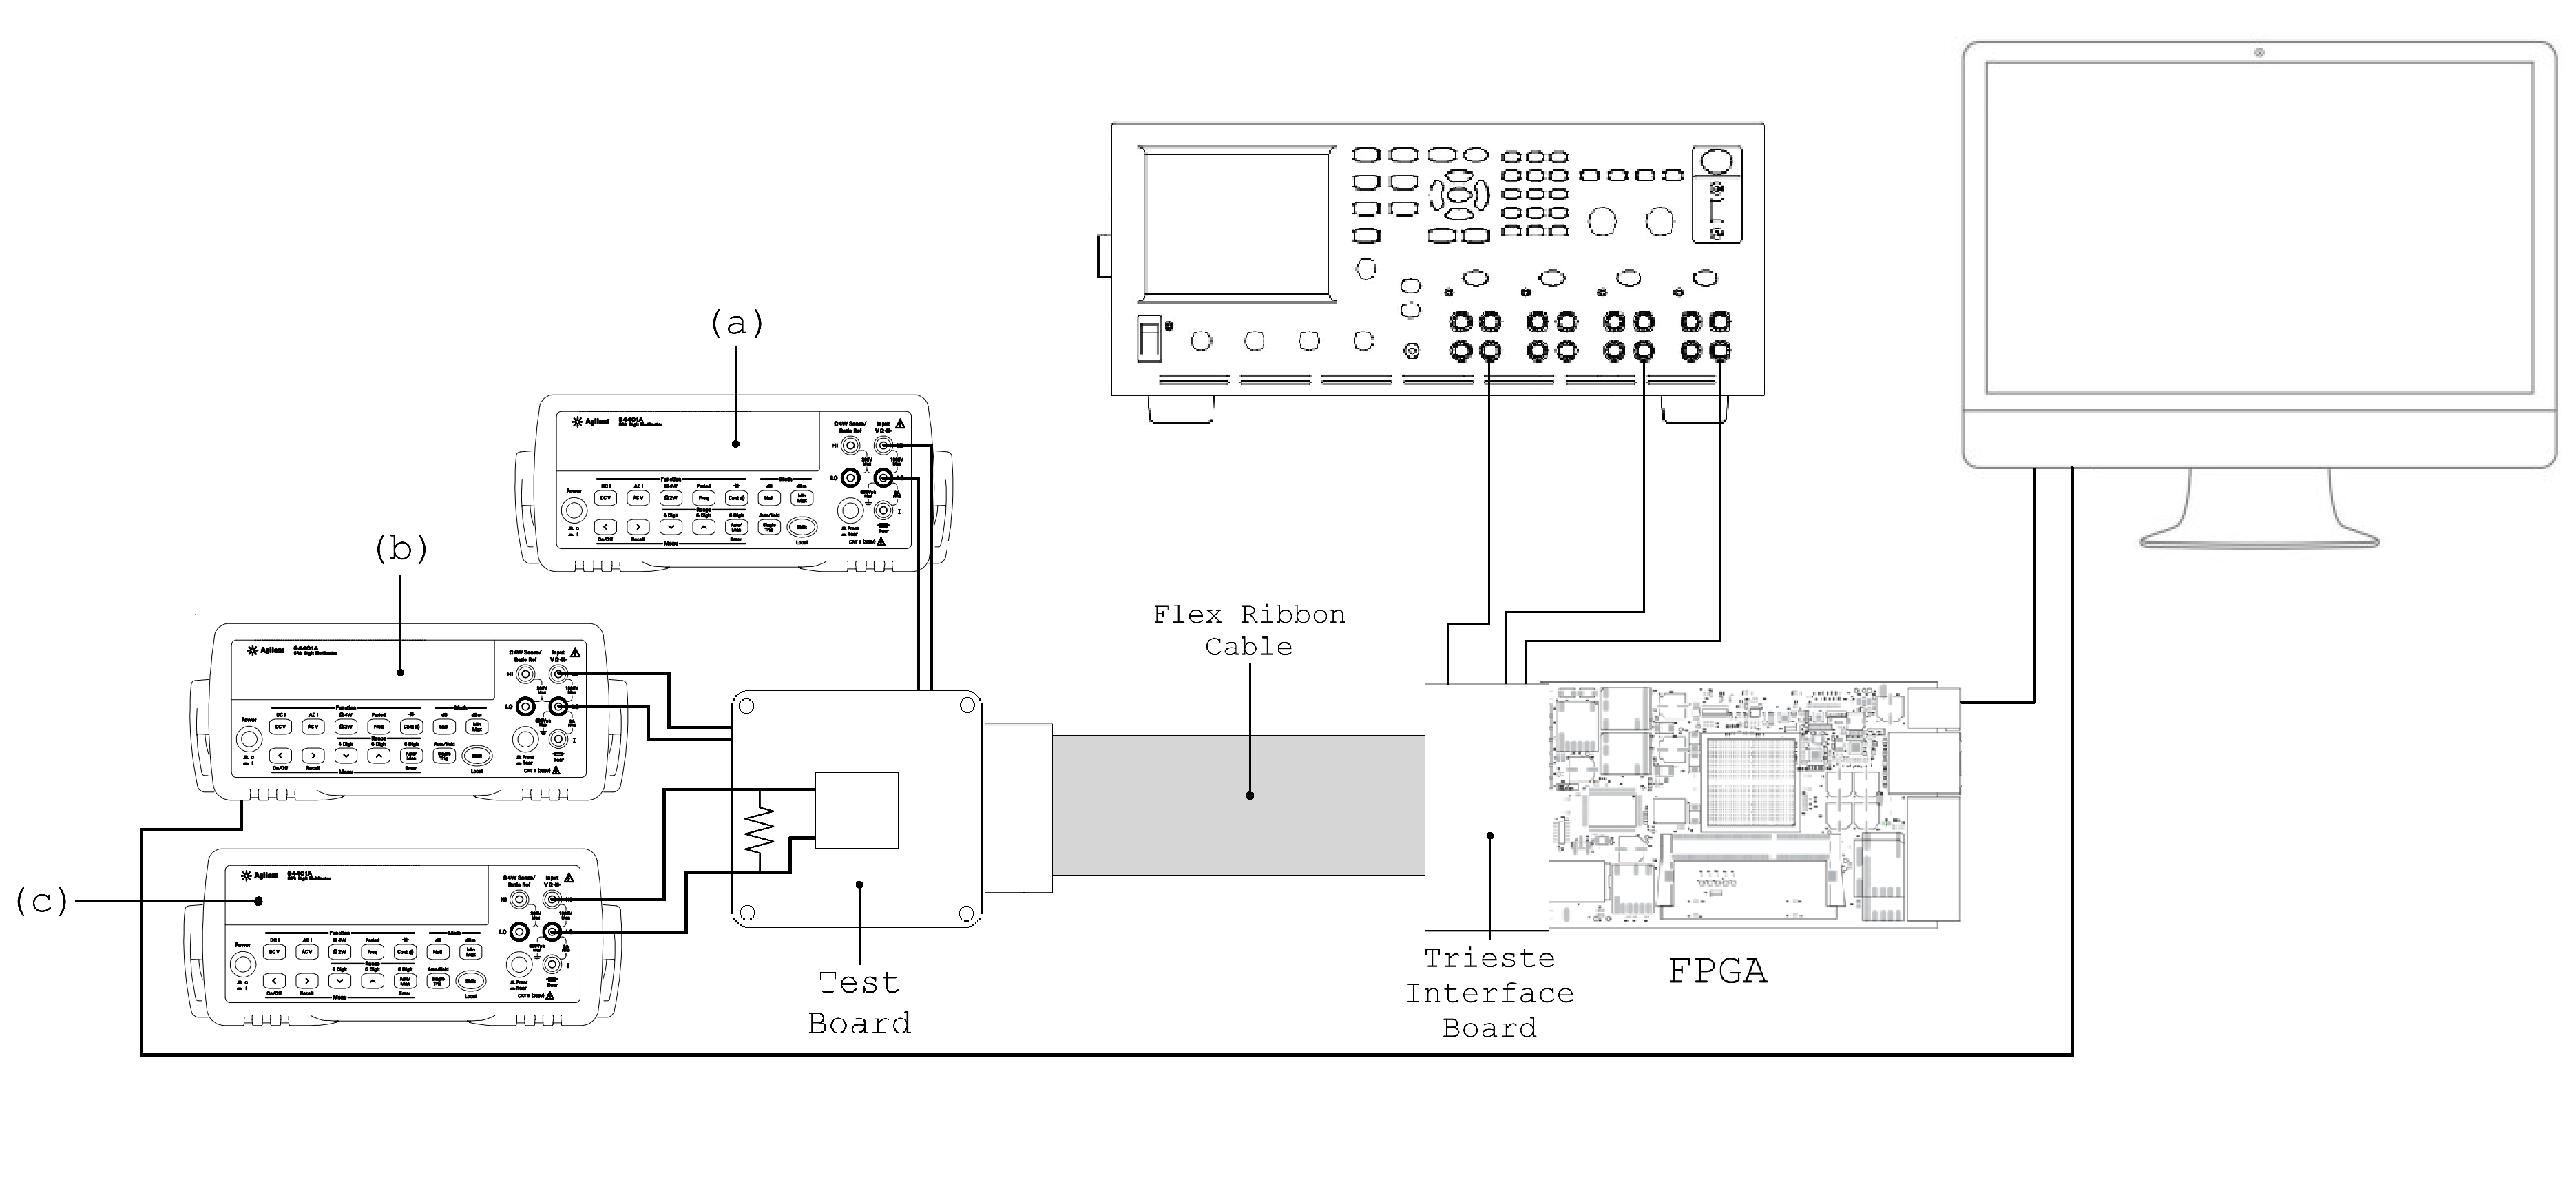
\includegraphics[width=1\textwidth]{Images/chap1/test_setup_test_board_csavrefgm_auto.png}
    \caption{SLIDER32 ASIC test board setup \texttt{1}.}
    \label{figTESTBOARDsetup1}
\end{figure}

\begin{figure}[h!]
    \centering
    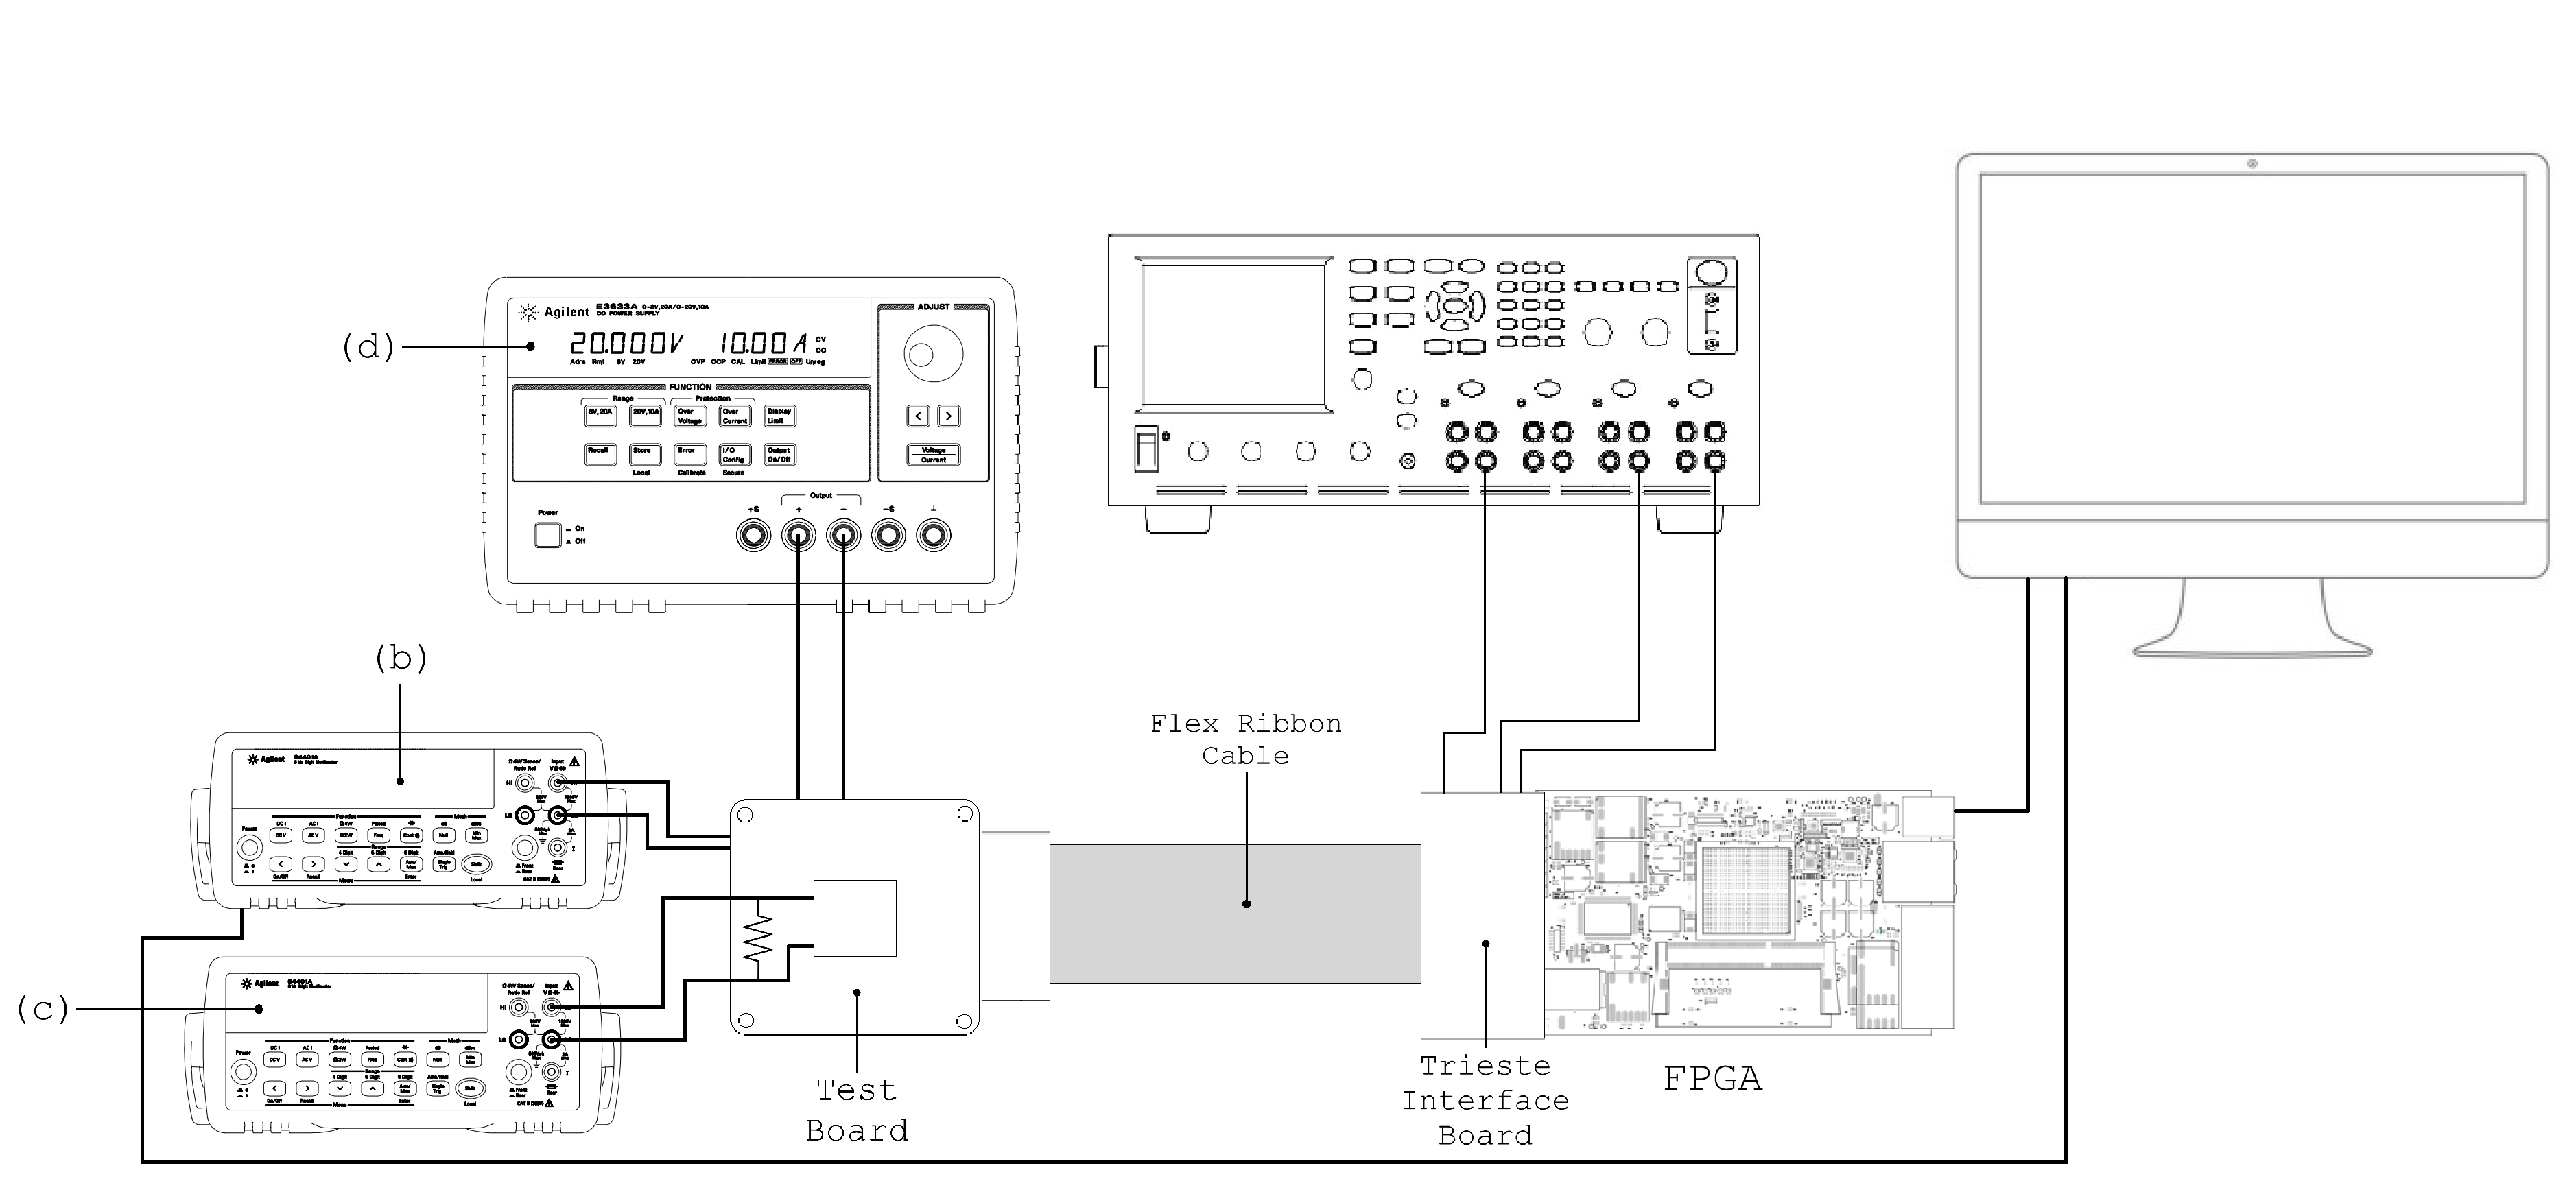
\includegraphics[width=1\textwidth]{Images/chap1/test_setup_test_board_csavrefgm_530mv.png}
    \caption{SLIDER32 ASIC test board setup \texttt{2}.}
    \label{figTESTBOARDsetup2}
\end{figure}

\par
\noindent
Both variants comprise the components discussed in the following.

\begin{itemize}
    \itemsep0em 
    \item A custom designed test board that allows tests to be performed on the ASIC without having to solder it to the board and then desolder it. This is made possible by a specific test socket that allows the ASIC to be mounted and removed without having to solder it to the test board. This solution also allows several ASICs to be tested using a single board, although being not being the case of the proposed measurements, that involved only ASIC No. \texttt{536}.
    \item A Keysight N6705C DC Power analyser providing both analog and digital voltages to the test board. \hyperref[figKeysightFEBtb]{Figure \ref{figKeysightFEBtb}} shows a screen capture of the power supply. Specifically, channel \texttt{1} provides the analog supply voltage (\SI{2.4}{\volt}), channel \texttt{3} provides the digital supply voltage (\SI{2.4}{\volt}) and channel \texttt{4} the 16-bit calibration DAC supply voltage (\SI{3.6}{\volt}).
    
    \begin{minipage}{\linewidth}
    \vspace{0.4cm}
        \centering
        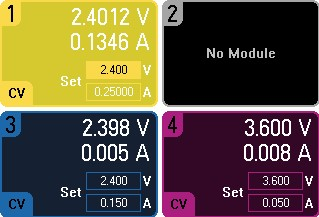
\includegraphics[width=0.5\textwidth]{Images/chap1/power_supply_screen_TB.jpg}
        \captionof{figure}{Keysight N6705C DC power analyser displayed voltages and currents on channels \texttt{1}, \texttt{3} and \texttt{4}.}
        \label{figKeysightFEBtb}
        \vspace{0.4cm}
    \end{minipage}
    
    \item An interface board specifically designed to route the power supplies and the signals trough the flex ribbon cable to the test board.
    \item A flex ribbon cable connecting the interface board to the main test board.
    \item An ALTERA Cyclone V Field Programmable Gate Array (FPGA).
    \item A PC running a Python-based testing program called \texttt{GAPS\_ModuleTester}, currently in its 4th version, connected to the FPGA via two Universal Serial Bus (USB) cables. This software has been specifically developed to perform a series of tests on the SLIDER32 ASIC and it is later described in \hyperref[sec21]{Section \ref{sec21}}.
    \item An Agilent 34401A digital multimeter \texttt{(b)} used to measure the global threshold voltage generated by an 8-bit DAC described in \hyperref[thresholdVoltageANALYSIS]{Section \ref{thresholdVoltageANALYSIS}}.
    \item An Agilent 34401A digital multimeter \texttt{(c)} used to measure the reference current as a voltage drop across a \SI{18}{\kilo\ohm} resistor mounted on the test board.
\end{itemize}

\par
Specific to version \texttt{1} of the test setup is the Agilent 34461A digital multimeter \texttt{(a)} that has been used to measure the \texttt{CSAVrefGM} voltage, automatically regulated by a bandgap with respect to the temperature at which the system operates in order to guarantee the correct gain of the readout channel.

\par
Version \texttt{2} of the test setup employs a Keysight E3631A DC power supply \texttt{(d)} in order to force the \texttt{CSAVrefGM} voltage to a fixed \SI{530}{\milli\volt} value. This voltage corresponds to the one provided by the bandgap at a temperature of \SI{-40}{\celsius}.

\par
The test board has been placed in a climate chamber (model ACS DY110) at temperatures spanning from \SI{-40}{\celsius} to \SI{30}{\celsius} with \SI{10}{\celsius} increments. The \SI{-40}{\celsius} to \SI{-30}{\celsius} region has been spanned with \SI{2}{\celsius} increments. In each test, before performing a test session, the climate chamber has been maintained at the desired temperature for 15 minutes in order to ensure that the electronics reached the correct temperature.

%-------------------------------------------------------------------------------
%	Current reference analysis
%-------------------------------------------------------------------------------

\section{Current reference}

The analog front-end channel designed for the readout of the Si(Li) detectors of the GAPS experiment is comprised of several blocks, as discussed in detail in \hyperref[secGAPSfrontend]{Appendix \ref{secGAPSfrontend}}. Each element of the channel requires one or more current references to be properly biased. These references should remain  constant regardless of external conditions like temperature, variations in the ASIC supply voltage and process parameter mismatch during fabrication. To comply with this requirement, a solution where the reference currents are generated starting from a precise Process, Voltage and Temperature (PVT) voltage reference has been adopted. Starting from this voltage, a 3-bit adjustable current can be obtained. This reference value has been chosen to be \SI{5}{\micro\ampere}.

\begin{figure}[h!]
    \centering
    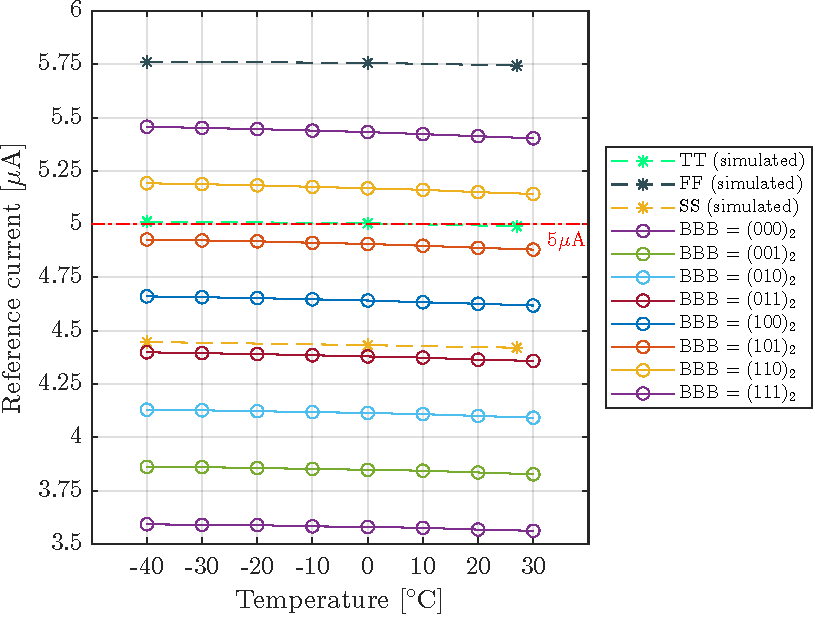
\includegraphics[width=0.7\textwidth]{Images/chap1/results/BGR_current/BGR_current_Xtemp_all-BBB.pdf}
    \caption{Reference current values for a given bias setting with respect to temperature varying from \SI{-40}{\celsius} to \SI{30}{\celsius} with \SI{10}{\celsius} increments.}
    \label{figBGRplotsXtempall}
\end{figure}

\par
A complete set of measurements of the reference current is shown in \hyperref[figBGRplotsXtempall]{Figure \ref{figBGRplotsXtempall}}. It has been taken by varying both the temperature from \SI{-40}{\celsius} to \SI{30}{\celsius} and the bias setting on all the 8 possible values. It can be seen that, for a given bias setting expressed as a combination of 3 bits (\texttt{BBB}), the reference current remains almost constant with the temperature and experiences a variation that is presented in \hyperref[tableBGRvariation]{Table \ref{tableBGRvariation}}. The plot also shows the trend of the reference current as predicted by simulations in 3 different CMOS process corners, namely \textit{Typical-Typical} (TT), \textit{Fast-Fast} (FF) and \textit{Slow-Slow} (SS).

\par
The reference current has been evaluated by measuring the voltage drop across the resistor $R_{\textit{3}}$ on the test board, a 0603 SMD resistor with \SI{0.1}{\percent} tolerance and \SI{10}{ppm/\celsius} temperature coefficient. The current value has been calculated as

\begin{equation}
    I_{ref} = \frac{V_{ref}}{R_{\textit{3}}}
\end{equation}

It is possible to see that, among all bias settings (\texttt{BBB}), the one being the closest to the \SI{5}{\micro\ampere} reference value is \texttt{101} at almost every temperature considered, thus validating the choice of using this bias setting as the default one in all the other tests performed.

\begin{table}[h!]
    \centering
    \begin{tabular}{c c c c} 
        \Xhline{2\arrayrulewidth}
        \multicolumn{1}{p{2.6cm}}{\T \centering Bias setting $[\texttt{BBB}]$ } & 
        \multicolumn{1}{p{3.2cm}}{\centering Reference current \\ at \SI{-40}{\celsius} $[\SI{}{\milli\ampere}]$} &
        \multicolumn{1}{p{3.2cm}}{\centering Reference current \\ at \SI{30}{\celsius} $[\SI{}{\milli\ampere}]$} & 
        \multicolumn{1}{p{1.8cm}}{\centering Variation \\ $[\%]$ \B} \\
        \hline
        000 & 3.59 & 3.56 & 0.85 \T\B \\
        001 & 3.86 & 3.83 & 0.90 \T\B \\
        010 & 4.13 & 4.09 & 0.91 \T\B \\
        011 & 4.40 & 4.36 & 0.92 \T\B \\
        100 & 4.66 & 4.62 & 0.92 \T\B \\
        101 & 4.93 & 4.88 & 0.96 \T\B \\
        110 & 5.19 & 5.14 & 0.96 \T\B \\
        111 & 5.46 & 5.40 & 0.99 \T\B \\
        \Xhline{2\arrayrulewidth}
    \end{tabular}
    \caption{Reference current values and variations with respect to temperature from \SI{-40}{\celsius} to \SI{30}{\celsius} for each bias settings.}
    \label{tableBGRvariation}
\end{table}

\par
\hyperref[figBGRplotXbias]{Figure \ref{figBGRplotXbias}} proposes on the left the plot of the reference current at temperatures varying from \SI{-40}{\celsius} to \SI{30}{\celsius} with respect to the bias setting. On the right, the measurement at \SI{30}{\celsius} is compared with simulations and a previously taken measurement at a temperature of \SI{27}{\celsius}.

\begin{figure}[h!]
    \centering
    \begin{tabular}{cc}
        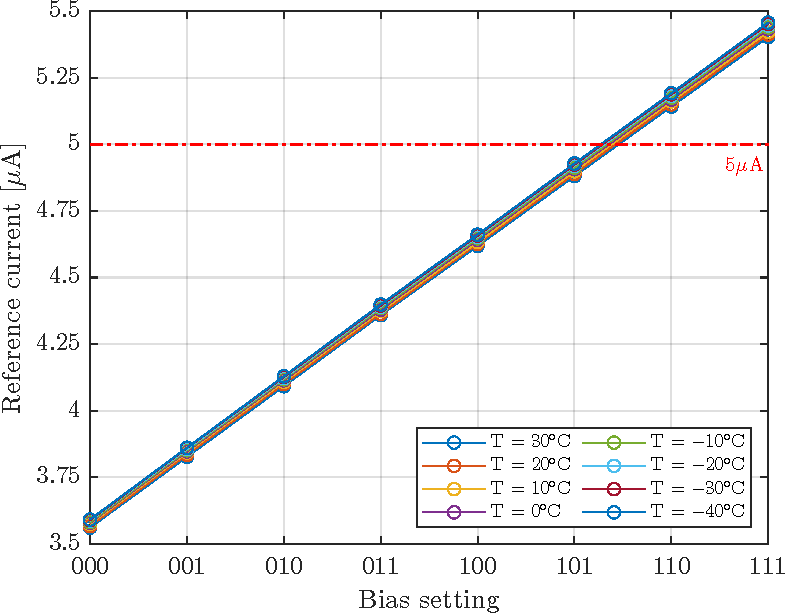
\includegraphics[width=0.475\textwidth]{Images/chap1/results/BGR_current/BGR_current_XBBB.pdf} & 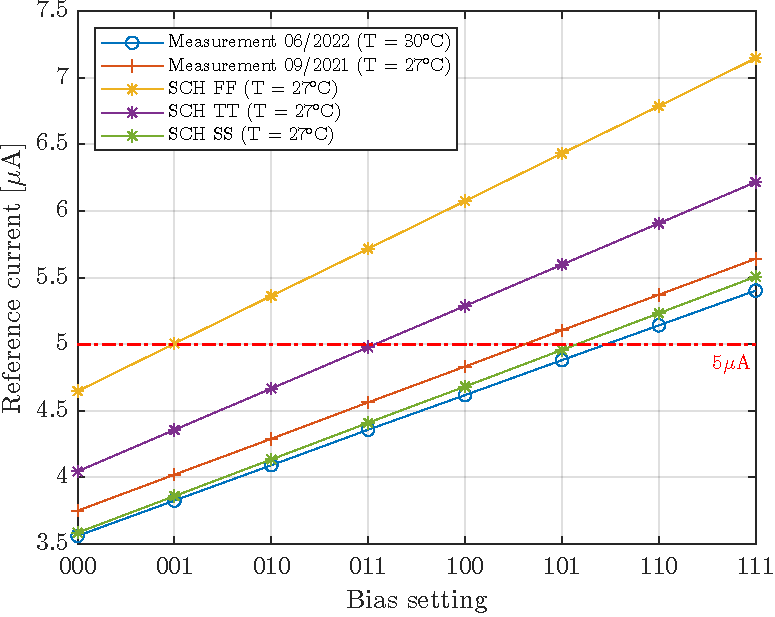
\includegraphics[width=0.475\textwidth]{Images/chap1/results/BGR_current/BGR_current_XBBB_27C_sim.pdf}\\
    \end{tabular}
    \caption{Current reference values given temperature with respect to bias setting (on the left) and with respect to simulations at \SI{27}{\celsius} (on the right).}
    \label{figBGRplotXbias}
\end{figure}

\par
\hyperref[figBGRplotsnormalised]{Figure \ref{figBGRplotsnormalised}} reports the normalised reference current measured at temperatures varying from \SI{-40}{\celsius} to \SI{30}{\celsius} and compared to the values coming from simulations in the same temperature range.

\begin{figure}[h!]
    \centering
    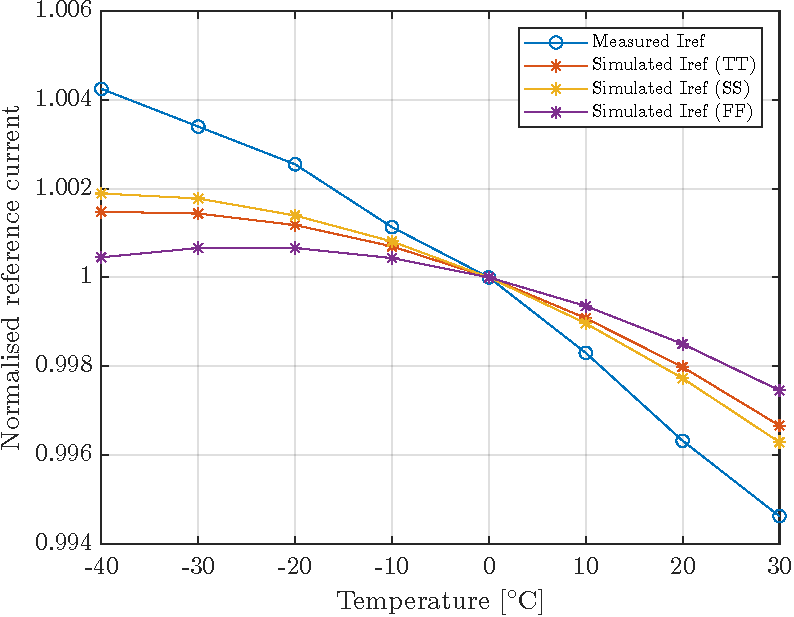
\includegraphics[width=0.7\textwidth]{Images/chap1/results/BGR_current/BGR_current_normal_Iref.pdf}
    \caption{Normalised current reference values compared to TT, FF and SS simulations with respect to temperature from \SI{-40}{\celsius} to \SI{30}{\celsius}.}
    \label{figBGRplotsnormalised}
\end{figure}

\par
The reference current measurements have also been evaluated by extracting the temperature coefficient, $\alpha$. The temperature coefficient can be defined as the ratio of change in resistance with respect to a variation of one degree in temperature and can be expressed as

\begin{equation}
    \alpha = \frac{1}{I_{T_{0}}} \cdot \frac{\Delta I}{\Delta T}
\end{equation}

\noindent
where $I_{T_{0}}$ represents the current value measured at a reference temperature of \SI{0}{\celsius} and $\Delta T$ is defined as the difference between the maximum and the minimum temperatures at which the measurements have been performed and it can be expressed as

\begin{equation}
    \Delta T = \lvert T_{max} - T_{min} \rvert
\end{equation}

\noindent
In the same way, $\Delta I$ represents the difference between the current measured at the minimum temperature, $T_{min}$, and that measured at the maximum temperature, $T_{max}$, and is defined as 

\begin{equation}
    \Delta I = I_{T_{min}}- I_{T_{max}}
\end{equation}

\noindent
In the specific case of the presented measurements and simulations, the temperature delta is equal to $\Delta T = \SI{70}{\celsius}$. The estimated temperature coefficients, expressed as \SI{}{ppm/\celsius}, are reported in \hyperref[tabtempcoefficients]{Table \ref{tabtempcoefficients}}. It is clear to see that the temperature coefficient of the measured reference current is above every one of the temperature coefficients evaluated over the readings coming from simulations in all of the 3 process corners. Nevertheless, the performances are adequate to what is required by the experiment.

\begin{table}[ht]
    \centering
    \begin{tabular}{c c} 
        \Xhline{2\arrayrulewidth}
        & $\alpha$ [\SI{}{ppm/\celsius}] \T\B \\
        \hline
        Measured & 137.42 \T\B \\
        TT model & 68.57 \T\B \\
        SS model & 80.00 \T\B \\
        FF model & 42.86 \T\B \\
        \Xhline{2\arrayrulewidth}
    \end{tabular}
    \caption{Estimated temperature coefficients.}
    \label{tabtempcoefficients}
\end{table}


%-------------------------------------------------------------------------------
%	Input-output channel trans-characteristic
%-------------------------------------------------------------------------------

\section{Input-output channel trans-characteristic}
\label{testboardFDT}

In this Section an analysis of the temperature effects on the Si(Li) detector analog readout channel input-output characteristic is given. The curve trend is mainly due to the Charge Sensitive Amplifier (CSA) circuit block, which is responsible for converting the incident charge on the Si(Li) detector into a voltage step signal that is subsequently supplied to the shaper, described in \hyperref[shaper]{Section \ref{shaper}}. 

\par
The CSA, whose schematic is shwon in \hyperref[figCSAschematic]{Figure \ref{figCSAschematic}}, is based on an inverting gain stage and a feedback capacitor where charge restoration is achieved by a continuous-time Krummenacher network \cite{krummenacher_1991_pixel}. 

\begin{figure}[h!]
    \centering
    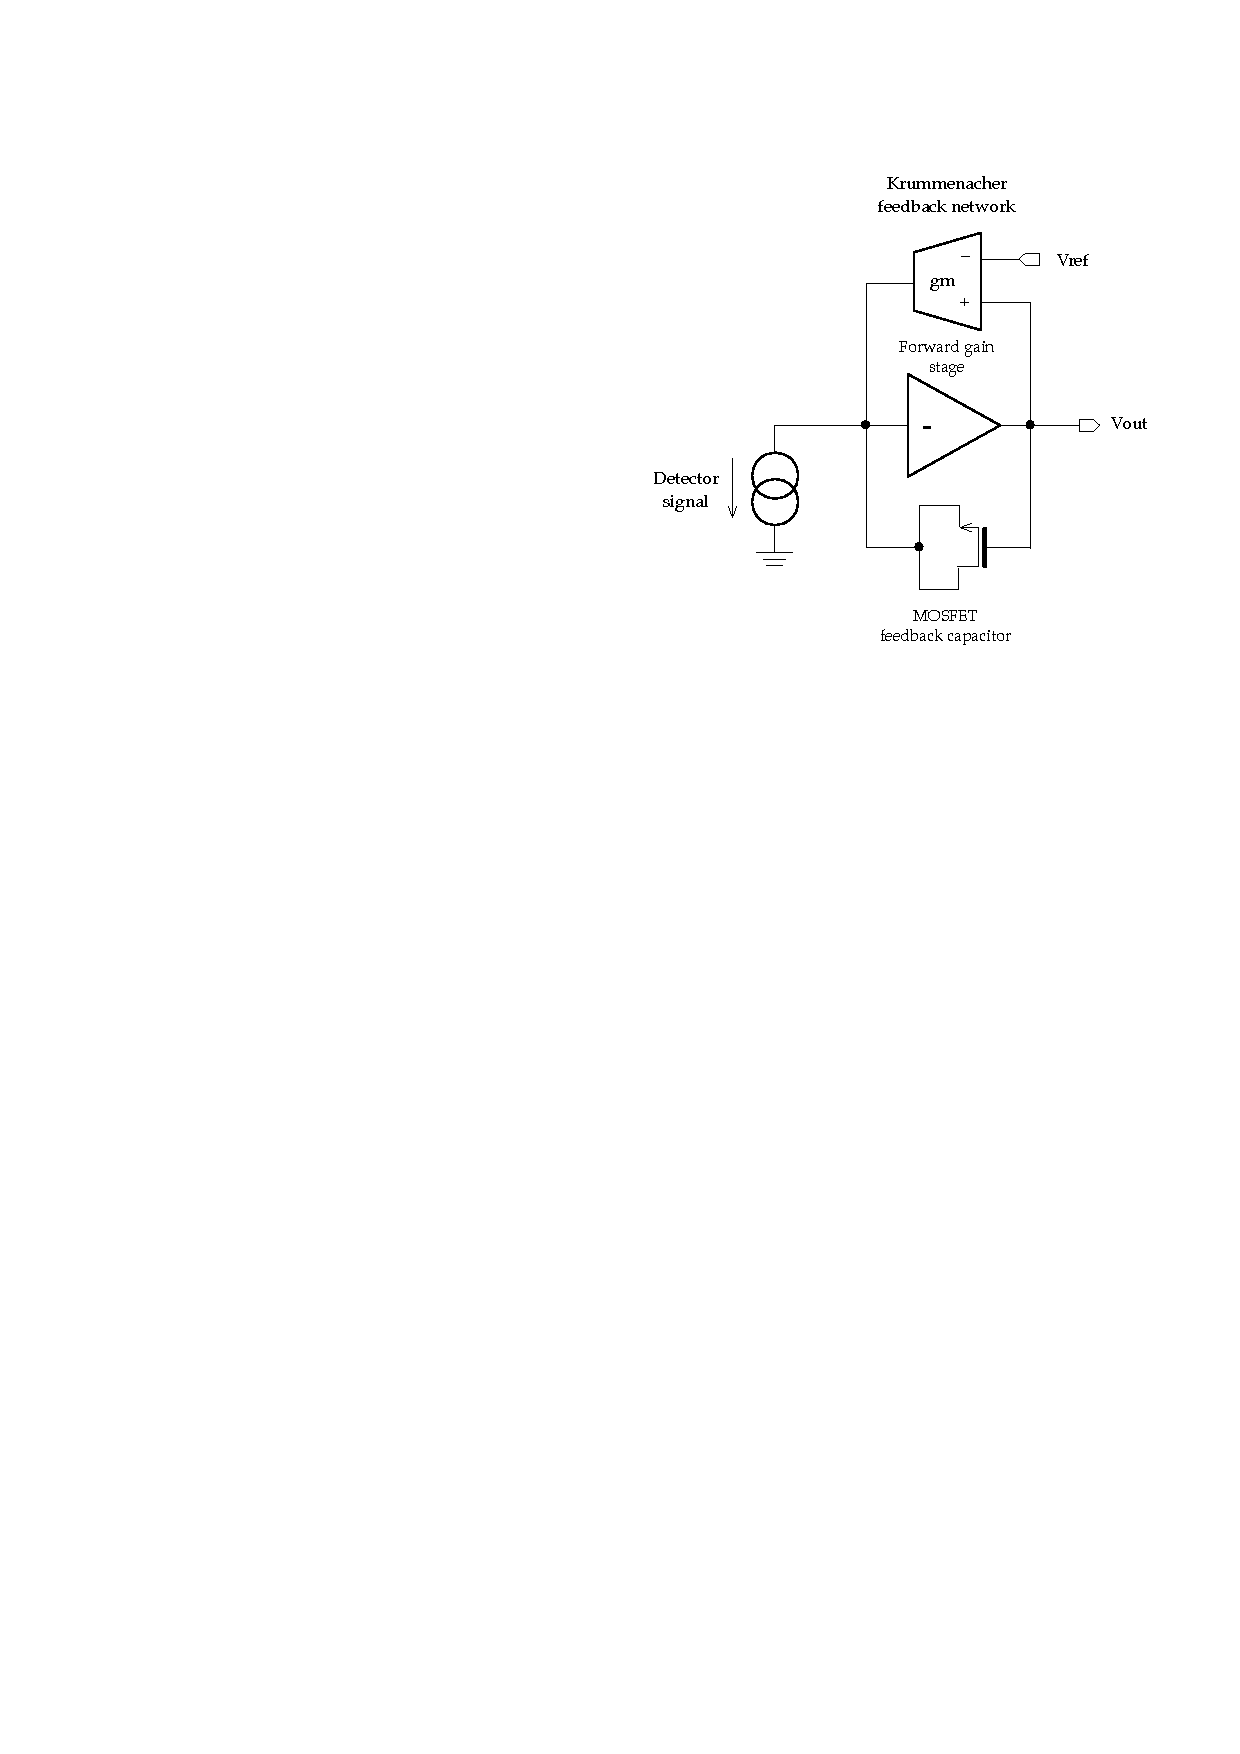
\includegraphics[width=0.65\textwidth]{Images/chap1/CSA_schematic.pdf}
    \caption{Schematic of the charge-sensitive preamplifier, with the forward gain stage, the nonlinear MOSFET capacitor and the Krummenacher feedback network.}
    \label{figCSAschematic}
\end{figure}

\par
The main feature of the CSA is the dynamic signal compression that is achieved by implementing the feedback capacitor with an NMOSFET operating in the inversion mode \cite{manghisoni_2018_dynamic}. In this transistor, source and drain are shorted to form the capacitor terminal connected to the amplifier input, while the gate terminal is connected to the output. At small signal amplitudes, the gate-to-channel voltage is smaller than the transistor threshold voltage and the capacitance is equal to the sum of gate-source and gate-drain overlap capacitances. At larger signal amplitudes, the gate-to-channel voltage becomes larger than the the transistor threshold and the capacitance increases including also the gate-to-channel capacitance. According to this mechanism, the feedback capacitance increases from \SI{175}{\femto\farad} at small input signal amplitudes to \SI{14.7}{\pico\farad} at large signal amplitudes. Since the gain of the CSA is proportional to the inverse of the capacitance this effect results in a gain that decreases with increase in the charge released in the detector.

\par
A reference voltage in the Krummenacher feedback network, denoted as $V_{ref}$ in \hyperref[figCSAschematic]{Figure \ref{figCSAschematic}} and referred to as \texttt{CSAVrefGM} in the following, makes it possible to adjust the amplifier output voltage, so that the signal amplitude at which the CSA switches from high to low gain can be finely tuned, compensating for process and temperature variations. In the nominal setting, the kink in the input-output characteristic occurs at an energy deposited in the detector of about \SI{1}{\mega\electronvolt}.

\par
In order to obtain the input-output characteristic of the CSA, the channel output must be sampled precisely at the peaking time, set by bit configuration \texttt{TTT}, that for the presented measurements has been chosen to be $\tau_{p} = \SI{0.98}{\micro\second}$ (peaking time 4, meaning \texttt{TTT} equal to \texttt{100}). The value of the injected charge is set by means of an external 16-bit DAC, therefore it ranges from 0 to \SI{65535}{DACu} (DAC unit). The code is converted in the equivalent energy value using the conversion factor of \SI{1}{DACu} = \SI{0.841}{\kilo\electronvolt}, whose value is later derived in \hyperref[eqConversionFactor]{Equation (\ref{eqConversionFactor})}, therefore the range can be equivalently expressed as spanning from 0 to \SI{50.46}{\mega\electronvolt}.

\begin{figure}[h!]
    \centering
    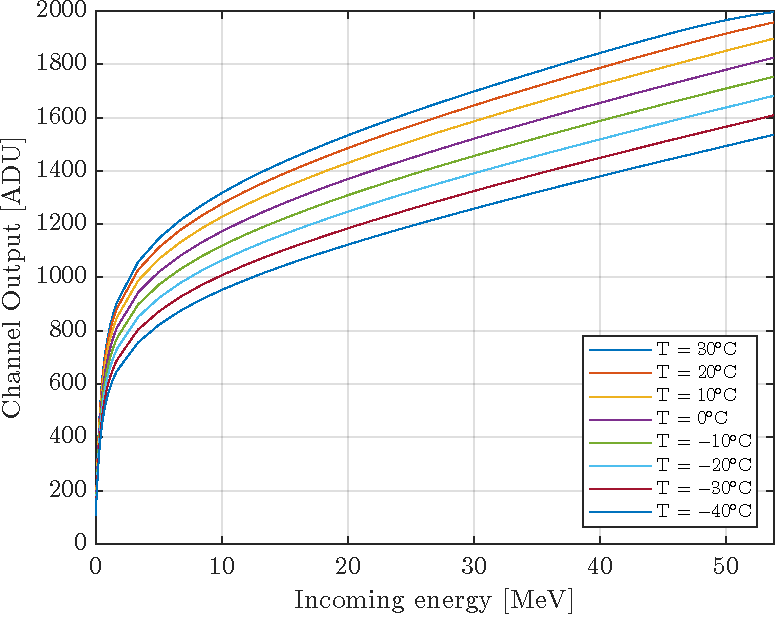
\includegraphics[width=0.68\textwidth]{Images/chap1/results/FDT/fdt_csavrefgm_auto_tau6_keV_0011.pdf}
    \caption{Mean input-output channel trans-characteristics with respect to temperature varying from \SI{-40}{\celsius} to \SI{30}{\celsius} and automatically regulated \texttt{CSAVrefGM} voltage.}
    \label{figFDTplotauto0011}
\end{figure}

\par
\hyperref[figFDTplotauto0011]{Figure \ref{figFDTplotauto0011}} shows the input-output trans-characteristic obtained as the mean of the 32 channels of the ASIC with respect to temperature ranging from \SI{-40}{\celsius} to \SI{30}{\celsius}. In this case, the \texttt{CSAVrefGM} voltage has been left free to automatically adapt to the given temperature and has been measured using the test setup \texttt{1} described in \hyperref[figTESTBOARDsetup1]{Figure \ref{figTESTBOARDsetup1}}. The CSA REFERENCE REGULATION setting (\texttt{HRRR} bits) has been set to \texttt{0011}. The first bit, \texttt{H}, is set to \texttt{0} when the ASIC is operated at \SI{-40}{\celsius} and to \texttt{1} when operated at room temperature. The last three bits, \texttt{RRR}, allow to set the charge sensitive amplifier reference.

\noindent
The \texttt{CSAVrefGM} values measured at each temperature are presented in \hyperref[tablecsavref]{Table \ref{tablecsavref}}. It comprises measurements taken with \texttt{HRRR} respectively set to \texttt{0011} and \texttt{0111} and the relative percentage variation between the two. It is of immediate comprehension that neither configuration is capable of reaching the desired \SI{530}{\milli\volt} at \SI{-40}{\celsius}. It is in fact necessary to set \texttt{RRR} to \texttt{111} in order to get the closest possible to the reference value.

\begin{table}[ht]
    \centering
    \begin{tabular}{c c c c} 
        \Xhline{2\arrayrulewidth}
        \multirow{2}{*}{Temperature [\SI{}{\celsius}]} \T & \multicolumn{2}{p{5cm}}{\centering \texttt{CSAVrefGM} $[\SI{}{\milli\volt}]$} \T & \multirow{2}{*}{Variation [\SI{}{\percent}]} \\
        \cline{2-3}
        & \texttt{HRRR = 0011} & \texttt{HRRR = 0111} \B\\
        \hline
        30 & 360.5 & 370.9 & 2.80 \T\B \\
        20 & 383.1 & 392.0 & 2.27 \T\B \\
        10 & 405.3 & 413.8 & 2.05 \T\B \\
        0 & 432.1 & 436.3 & 6.73 \T\B \\
        -10 & 450.5 & 458.4 & 1.72 \T\B \\
        -20 & 473.2 & 480.6 & 1.54 \T\B \\
        -30 & 495.1 & 504.3 & 1.82 \T\B \\
        -40 & 517.5 & 525.8 & 1.58 \T\B \\
        \Xhline{2\arrayrulewidth}
    \end{tabular}
    \caption{\texttt{CSAVrefGM} voltage measured at temperatures varying from \SI{-40}{\celsius} to \SI{30}{\celsius} with CSA REFERENCE REGULATION bits set to \texttt{0011} and \texttt{0111} respectively.}
    \label{tablecsavref}
\end{table}

\hyperref[figFDTplot530mV]{Figure \ref{figFDTplot530mV}} shows the mean input-output channel trans-characteristics calculated over the 32 channels of the ASIC given temperatures ranging from \SI{-40}{\celsius} to \SI{30}{\celsius}. In this case, the \texttt{CSAVrefGM} has been set to a fixed value of \SI{530}{\milli\volt} using the test setup \texttt{2} described in \hyperref[figTESTBOARDsetup2]{Figure \ref{figTESTBOARDsetup2}}. It is possible to notice that by fixing the voltage to the automatically regulated value at \SI{-40}{\celsius} regardless of the temperature, the channel transfer function assumes an unwanted trend.  

\begin{figure}[h!]
    \centering
    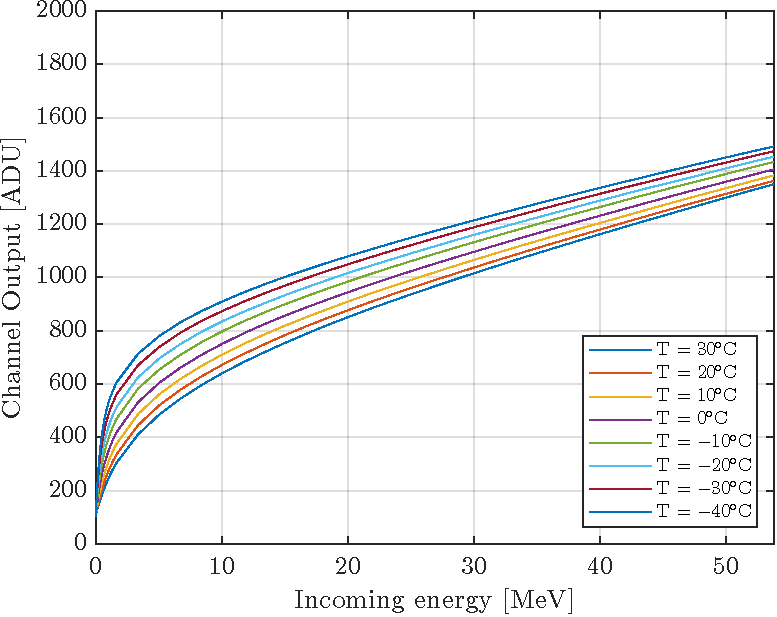
\includegraphics[width=0.68\textwidth]{Images/chap1/results/FDT/fdt_csavrefgm_530mV_tau6_keV.pdf}
    \caption{Mean input-output channel trans-characteristics given temperatures varying from \SI{-40}{\celsius} to \SI{30}{\celsius} and \texttt{CSAVrefGM} voltage fixed to \SI{530}{\milli\volt}.}
    \label{figFDTplot530mV}
\end{figure}

\par
As it can be seen from the charts, the channel input-output trans-characteristic is a non-linear function that can be described as an almost piecewise linear function whose sensitivity is determined by the dynamic compression feature of the CSA. Through this non-linearity the resolution of the signals changes as a function of the charge generated by the energy release of the incident particle in the detector: in a low energy range, the resolution of the signal must be high and, consequently, the charge signal must be amplified adequately and vice versa in the high energy range. This implies that in the first segment the transfer function has a high slope. In the high energy range, however, the required resolution is not so stringent, consequently the gain of the transfer function is less than that in the first section. The channel transfer function can therefore be divided into two regions, based on the incoming energy:

\begin{itemize}
    \itemsep0em
    \item \textit{Low energy region}: Also known as X-ray detection region, it ranges from approximately 10 to \SI{100}{\kilo\electronvolt}.
    \item \textit{High energy region}: Also described as muon detection region, it spans an energy range comprised between 40 and \SI{55}{\mega\electronvolt}.
\end{itemize}

\noindent
In both X-ray and muon detection regions, the characteristic exhibits a linear behaviour and can be expressed as

\begin{equation}
    y = p + g \cdot x
    \label{FDTlinearModel}
\end{equation}

\noindent
where

\begin{itemize}
    \itemsep0em
    \item \textbf{y} [\SI{}{ADU}] (Analog Digital Unit) is the channel output.
    \item \textbf{p} [\SI{}{ADU}] is the pedestal, which consists of a repeated sampling of the channel output without charge injected.
    \item \textbf{g} [\SI{}{ADU/\kilo\electronvolt}] is the channel gain.
    \item \textbf{x} [\SI{}{\kilo\electronvolt}] is the input energy.
\end{itemize}

The effect of temperature variation on the channel transfer function has been studied by evaluating gain and pedestal in both X-ray and muon detection regions. For each of the two parameters, a linear regression model has been defined in order to study the trend on both gain and pedestal with respect to temperature ranging from \SI{-40}{\celsius} to \SI{30}{\celsius}, which has been demonstrated to have an almost perfect linear trend. For the gain analysis, the following linear regression model has been defined.

\begin{equation}
    g = g_{\textit{0}} + g_{\textit{1}} \cdot (T - T_{\textit{0}})
    \label{equationGain}
\end{equation}

\noindent
The intercept $g_{\textit{0}}$ is measured in \SI{}{ADU/\kilo\electronvolt}, the slope $g_{\textit{1}}$ in ADU \SI{}{\kilo\electronvolt^{-1}} \SI{}{\celsius^{-1}} and the reference temperature has been set to $T_{\textit{0}} = \SI{0}{\celsius}$. For the study of the gain in the high-energy region, $g_{0}$ is reported in \SI{}{ADU/\mega\electronvolt}, while $g_{1}$ is expressed in ADU \SI{}{\mega\electronvolt^{-1}} \SI{}{\celsius^{-1}}. Similarly, the following linear regression model has been defined for pedestal analysis.

\begin{equation}
    p = p_{\textit{0}} + p_{\textit{1}} \cdot (T - T_{\textit{0}})
\end{equation}

\noindent
The intercept $p_{\textit{0}}$ is measured in \SI{}{ADU}, the slope $p_{\textit{1}}$ in \SI{}{ADU/\celsius} and the reference temperature has been set to $T_{\textit{0}} = \SI{0}{\celsius}$. 

\par
\hyperref[tableFDTgainpedestal1]{Table \ref{tableFDTgainpedestal1}} provides the linear regression model coefficients for both gain and pedestal obtained upon the mean channel input-output characteristics measured at temperatures ranging between \SI{-40}{\celsius} and \SI{30}{\celsius}.

\begin{table}[ht]
    \centering
    \begin{tabular}{c c c c c c c} 
        \Xhline{2\arrayrulewidth}
        & \multicolumn{3}{c}{Gain} & \multicolumn{3}{c}{Pedestal} \T\B \\
        
        \hline
        & \multicolumn{1}{p{1.3cm}}{\centering $g_{\textit{0}}$\T \\\vspace{0.1cm} $\left[\frac{\SI{}{ADU}}{\SI{}{\kilo\electronvolt}}\right]$\vspace{0.1cm}\B} & \multicolumn{1}{p{1.3cm}}{\centering $g_{\textit{1}}$\T \\\vspace{0.1cm} $\left[\frac{\SI{}{ADU}}{\SI{}{\kilo\electronvolt\celsius}}\right]$\B} & \multirow{2}{*}{R$^{2}$} & \multicolumn{1}{p{1.3cm}}{\centering $p_{\textit{0}}$\T \\\vspace{0.1cm} $\SI{}{[ADU]}$\B} & \multicolumn{1}{p{1.3cm}}{\centering $p_{\textit{1}}$\T \\\vspace{0.1cm} $\left[\frac{\SI{}{ADU}}{\SI{}{\celsius}}\right]$\B} &  \multirow{2}{*}{R$^{2}$} \T\B \\
        \hline
        
        \multicolumn{1}{p{4.5cm}}{\centering X-ray detection region \T \\ (10$\div$\SI{100}{\kilo\electronvolt})} & \multirow{2}{*}{1.25} & \multirow{2}{*}{0.006} & \multirow{2}{*}{0.997} & \multirow{2}{*}{182.32} & \multirow{2}{*}{0.651} & \multirow{2}{*}{0.985} \\
        \multicolumn{1}{p{4.5cm}}{\centering Muon detection region \B \\ (40$\div$\SI{55}{\mega\electronvolt})} & \multirow{2}{*}{12.27} & \multirow{2}{*}{0.024} & \multirow{2}{*}{0.989} & \multirow{2}{*}{1738} & \multirow{2}{*}{6.778} & \multirow{2}{*}{0.999} \T\B \\
        \Xhline{2\arrayrulewidth}
    \end{tabular}
    \caption{Gain and pedestal linear regression models coefficients obtained from measurements with automatically generated \texttt{CSAVrefGM} voltage and \texttt{HRRR} set to \texttt{0011}.}
    \label{tableFDTgainpedestal1}
\end{table}

\noindent
The channel peaking time has been set to $\tau_{p} = \SI{0.98}{\micro\second}$ (peaking time 4, \texttt{TTT} set to \texttt{100}), with \texttt{CSAVrefGM} voltage automatically generated and \texttt{HRRR} set to \texttt{0011}.

\par
\hyperref[tableFDTgainpedestal530]{Table \ref{tableFDTgainpedestal530}} presents the same linear regression models coefficients but in the case of fixed \texttt{CSAVrefGM} voltage, that has been set to \SI{530}{\milli\volt}.

\begin{table}[ht]
    \centering
    \begin{tabular}{c c c c c c c} 
        \Xhline{2\arrayrulewidth}
        & \multicolumn{3}{c}{Gain} & \multicolumn{3}{c}{Pedestal} \T\B \\
        
        \hline
        & \multicolumn{1}{p{1.3cm}}{\centering $g_{\textit{0}}$\T \\\vspace{0.1cm} $\left[\frac{\SI{}{ADU}}{\SI{}{\kilo\electronvolt}}\right]$\vspace{0.1cm}\B} & \multicolumn{1}{p{1.3cm}}{\centering $g_{\textit{1}}$\T \\\vspace{0.1cm} $\left[\frac{\SI{}{ADU}}{\SI{}{\kilo\electronvolt\celsius}}\right]$\B} & \multirow{2}{*}{R$^{2}$} & \multicolumn{1}{p{1.3cm}}{\centering $p_{\textit{0}}$\T \\\vspace{0.1cm} $\SI{}{[ADU]}$\B} & \multicolumn{1}{p{1.3cm}}{\centering $p_{\textit{1}}$\T \\\vspace{0.1cm} $\left[\frac{\SI{}{ADU}}{\SI{}{\celsius}}\right]$\B} &  \multirow{2}{*}{R$^{2}$} \T\B \\
        \hline
        
        \multicolumn{1}{p{4.5cm}}{\centering X-ray detection region \T \\ (10$\div$\SI{100}{\kilo\electronvolt})} & \multirow{2}{*}{0.46} & \multirow{2}{*}{-0.012} & \multirow{2}{*}{0.992} & \multirow{2}{*}{128.66} & \multirow{2}{*}{-0.530} & \multirow{2}{*}{0.974} \T\B \\
        \multicolumn{1}{p{4.5cm}}{\centering Muon detection region \\ (40$\div$\SI{55}{\mega\electronvolt}) \B} & \multirow{2}{*}{12.61} & \multirow{2}{*}{0.033} & \multirow{2}{*}{0.997} & \multirow{2}{*}{1325.4} & \multirow{2}{*}{-2.406} & \multirow{2}{*}{0.988} \T\B \\
        \Xhline{2\arrayrulewidth}
    \end{tabular}
    \caption{Gain and pedestal linear regression models coefficients obtained from measurements with \texttt{CSAVrefGM} voltage set at a fixed value of \SI{530}{\milli\volt}.}
    \label{tableFDTgainpedestal530}
\end{table}

Graphs presented below show the trend of gain and pedestal with respect to temperature in the low and high energy regions for the configurations where \texttt{CSAVrefGM} is automatically adjusted (with \texttt{HRRR} set to \texttt{0011}) and set to \SI{530}{\milli\volt} respectively. The measurements were carried out by varying the temperature from \SI{-40}{\celsius} to \SI{30}{\celsius} in steps of \SI{10}{\celsius}, while the region between \SI{-40}{\celsius} and \SI{-30}{\celsius} was studied with steps of \SI{2}{\celsius}. 

% low energy gain
\begin{figure}[h!]
    \centering
    \begin{tabular}{cc}
        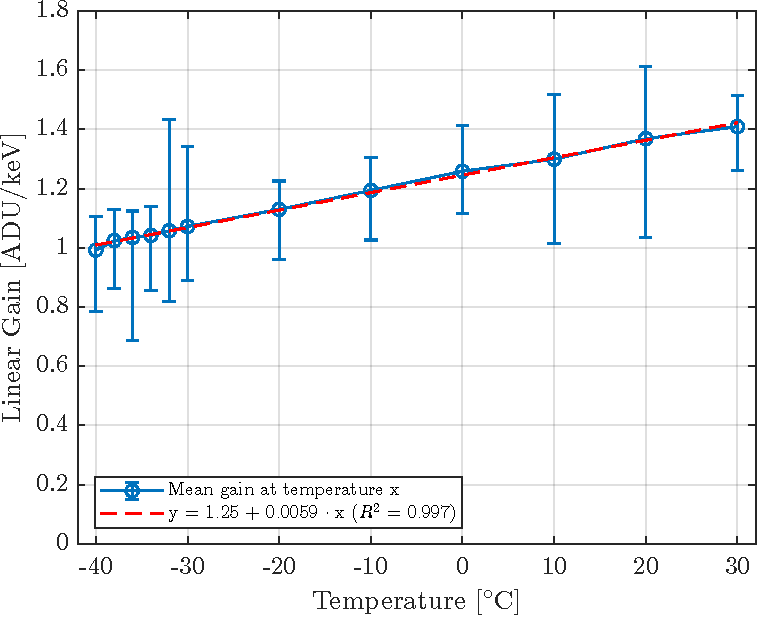
\includegraphics[width=0.475\textwidth]{Images/chap1/results/gain_pedestal/low_energy_gain_auto_0011.pdf} & 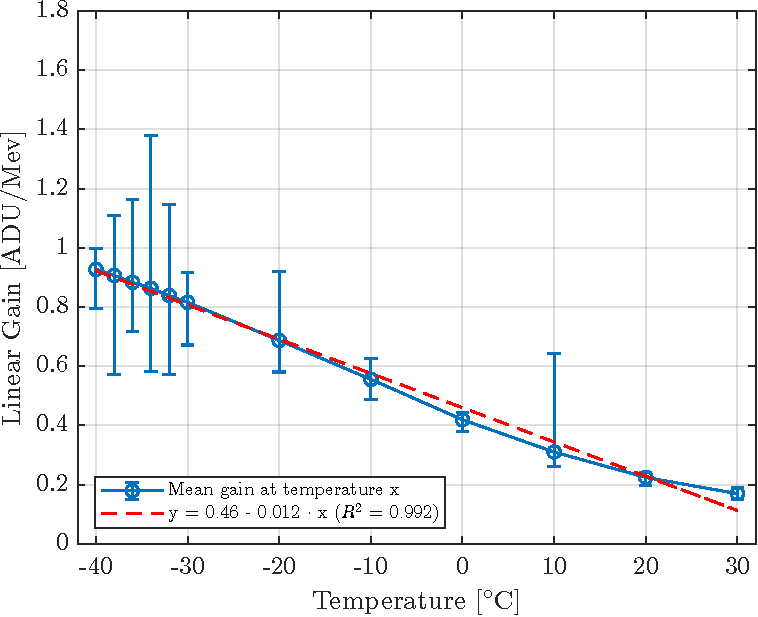
\includegraphics[width=0.475\textwidth]{Images/chap1/results/gain_pedestal/low_energy_gain_530mV.pdf}\\
    \end{tabular}
    \caption{Low energy gain trend with respect to temperature from \SI{-40}{\celsius} to \SI{30}{\celsius} for automatically regulated \texttt{CSAVrefGM} voltage (on the left) and fixed to \SI{530}{\milli\volt} (on the right).}
    \label{figFDTgainLowEnergies}
\end{figure}

The effect of keeping the CSA regulation voltage fixed can be seen in \hyperref[figFDTgainLowEnergies]{Figure \ref{figFDTgainLowEnergies}}, which manifests itself in a decreasing gain trend at low energies. This can be explained by the fact that, when the \texttt{CSAVrefGM} voltage is fixed at \SI{530}{\milli\volt}, it deviates considerably from the automatically adjusted nominal value at temperatures above \SI{-40}{\celsius}, shown in \hyperref[tablecsavref]{Table \ref{tablecsavref}}, until it reaches a difference of approximately \SI{170}{\milli\volt} at \SI{30}{\celsius}, the result of which is evident from the trend of the transfer function in \hyperref[figFDTplot530mV]{Figure \ref{figFDTplot530mV}}.

\par
\hyperref[figFDTgainHighEnergies]{Figure \ref{figFDTgainHighEnergies}} shows the gain trend in the high energy region under the same conditions, presenting the configuration with automatically regulated \texttt{CSAVrefGM} voltage on the left and fixed to \SI{530}{\milli\volt} on the right.

% high energy gain
\begin{figure}[h!]
    \centering
    \begin{tabular}{cc}
        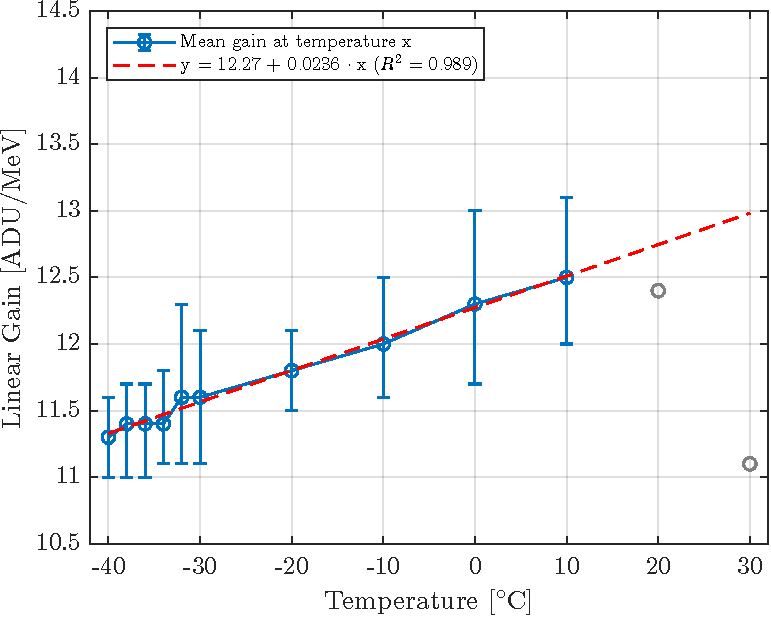
\includegraphics[width=0.475\textwidth]{Images/chap1/results/gain_pedestal/high_energy_gain_auto_0011.pdf} & 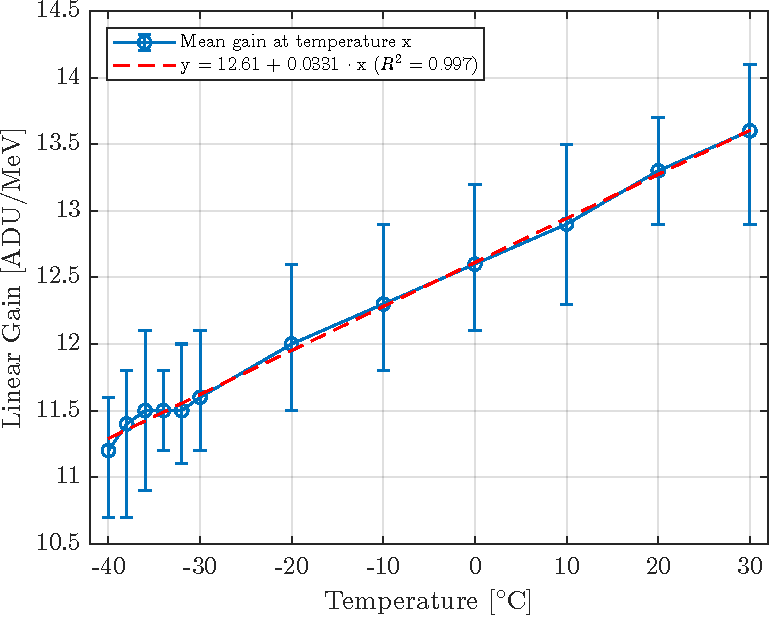
\includegraphics[width=0.475\textwidth]{Images/chap1/results/gain_pedestal/high_energy_gain_530mV.pdf}\\
    \end{tabular}
    \caption{High energy gain trend with respect to temperature from \SI{-40}{\celsius} to \SI{30}{\celsius} for automatically regulated \texttt{CSAVrefGM} voltage (on the left) and fixed to \SI{530}{\milli\volt} (on the right). The linear gain is expressed in \SI{}{ADU\per\mega\electronvolt}.}
    \label{figFDTgainHighEnergies}
\end{figure}

\noindent
It can be seen that, although $g_{0}$ assumes a value that is almost comparable between the two configurations, $g_{1}$ presents an increment of $\approx \SI{28.7}{\percent}$ when \texttt{CSAVrefGM} is set to \SI{530}{\milli\volt}, thus resulting in a higher increase in gain with respect to temperature. \hyperref[figFDTpedestalLowEnergies]{Figure \ref{figFDTpedestalLowEnergies}} and \hyperref[figFDTpedestalHighEnergies]{Figure \ref{figFDTpedestalHighEnergies}} present the trend of the pedestal as a function of temperature under the same conditions illustrated above.

% low energy pedestal
\begin{figure}[h!]
    \centering
    \begin{tabular}{cc}
        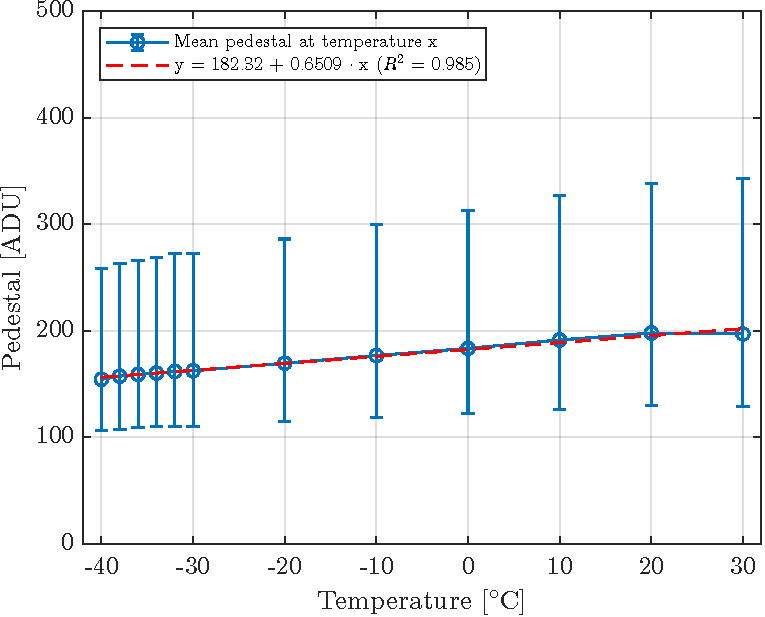
\includegraphics[width=0.475\textwidth]{Images/chap1/results/gain_pedestal/low_energy_pedestal_auto_0011.pdf} & 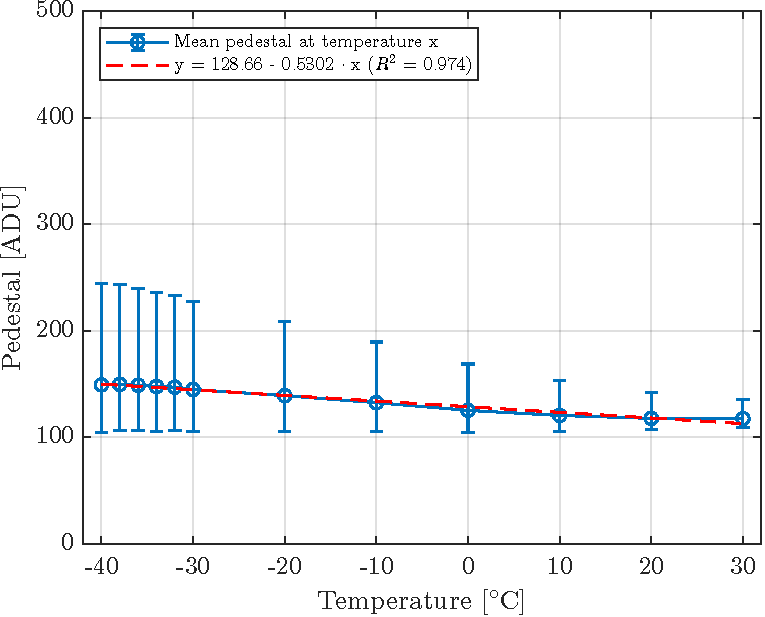
\includegraphics[width=0.475\textwidth]{Images/chap1/results/gain_pedestal/low_energy_pedestal_530mV.pdf}\\
    \end{tabular}
    \caption{Low energy pedestal trend with respect to temperature from \SI{-40}{\celsius} to \SI{30}{\celsius} for automatically regulated \texttt{CSAVrefGM} voltage (on the left) and fixed to \SI{530}{\milli\volt} (on the right).}
    \label{figFDTpedestalLowEnergies}
\end{figure}

% high energy pedestal
\begin{figure}[h!]
    \centering
    \begin{tabular}{cc}
        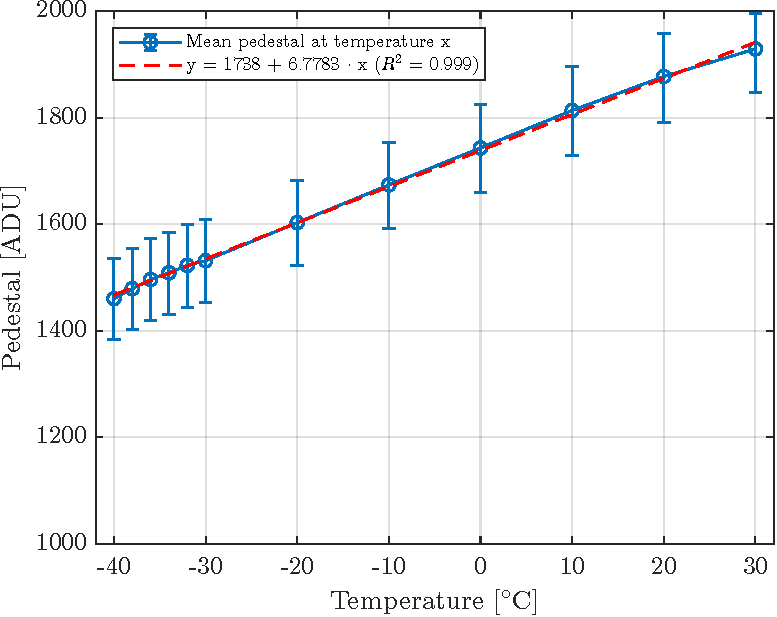
\includegraphics[width=0.475\textwidth]{Images/chap1/results/gain_pedestal/high_energy_pedestal_auto_0011.pdf} & 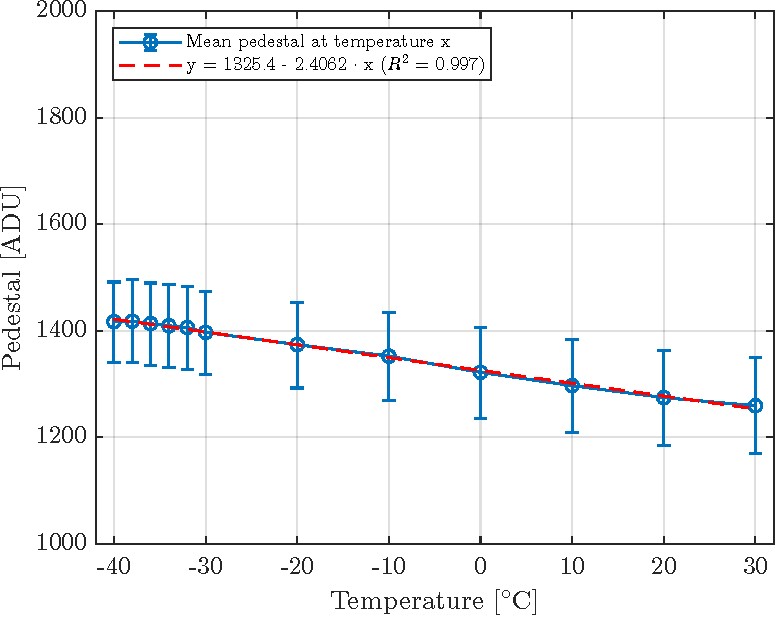
\includegraphics[width=0.475\textwidth]{Images/chap1/results/gain_pedestal/high_energy_pedestal_530mV.pdf}\\
    \end{tabular}
    \caption{High energy pedestal trend with respect to temperature from \SI{-40}{\celsius} to \SI{30}{\celsius} for automatically regulated \texttt{CSAVrefGM} voltage (on the left) and fixed to \SI{530}{\milli\volt} (on the right).}
    \label{figFDTpedestalHighEnergies}
\end{figure}

\par
Pedestal and gain measurements were used to study the variation in the position of the transfer function kink as temperature changes. In particular, \hyperref[figFDTkinkVariation]{Figure \ref{figFDTkinkVariation}} shows the interpolation curves of the transfer function in the low and high energy regions, previously referred to as \textit{X-ray} and \textit{muon} detection regions respectively. In particular, their intersection determines the point, expressed in \SI{}{\mega\electronvolt}, at which the change of slope occurs in the channel's input-output characteristic, which, in the particular example case, refers to the measurement obtained at a temperature of \SI{-40}{\celsius}. The two curves refer to the model shown in \hyperref[FDTlinearModel]{Equation (\ref{FDTlinearModel})} and the resolution of the system shown in \hyperref[FDTkinkSystem]{Equation (\ref{FDTkinkSystem})} allows the value of the kink at each temperature step to be determined as the intersection of the two straight lines that linearly approximate the transfer function in the high and the low energy region.

\begin{equation}
    \begin{cases}
        y = p_{LE} + g_{LE} \cdot x \\
        y = p_{HE} + g_{HE} \cdot x
    \end{cases}
    \label{FDTkinkSystem}
\end{equation}

\noindent
In particular, the subscript \textit{LE} refers to the model that describes the trend of the transfer function in the \textit{Low Energy} region, while the subscript \textit{HE} describes its trend in the \textit{High Energy} region. 

\par
Solving the system reported in \hyperref[FDTkinkSystem]{Equation (\ref{FDTkinkSystem})} allows the kink value expressed in \SI{}{\mega\electronvolt} to be obtained:

\begin{equation}
    x = \frac{p_{LE} - p_{HE}}{g_{HE} - g_{LE}}
\end{equation}

\par
From the graph shown in \hyperref[figFDTkinkVariationResult]{Figure \ref{figFDTkinkVariationResult}} it is possible to appreciate the kink trend of the channel transfer function as the temperature varies, for temperature values between \SI{-40}{\celsius} and \SI{30}{\celsius}. In particular, the kink trend is shown in red when the \texttt{CSAVrefGM} voltage is fixed at \SI{530}{\milli\volt}, while it is shown in blue when this voltage is automatically varied on the basis of temperature.

\begin{figure}[h!]
    \centering
    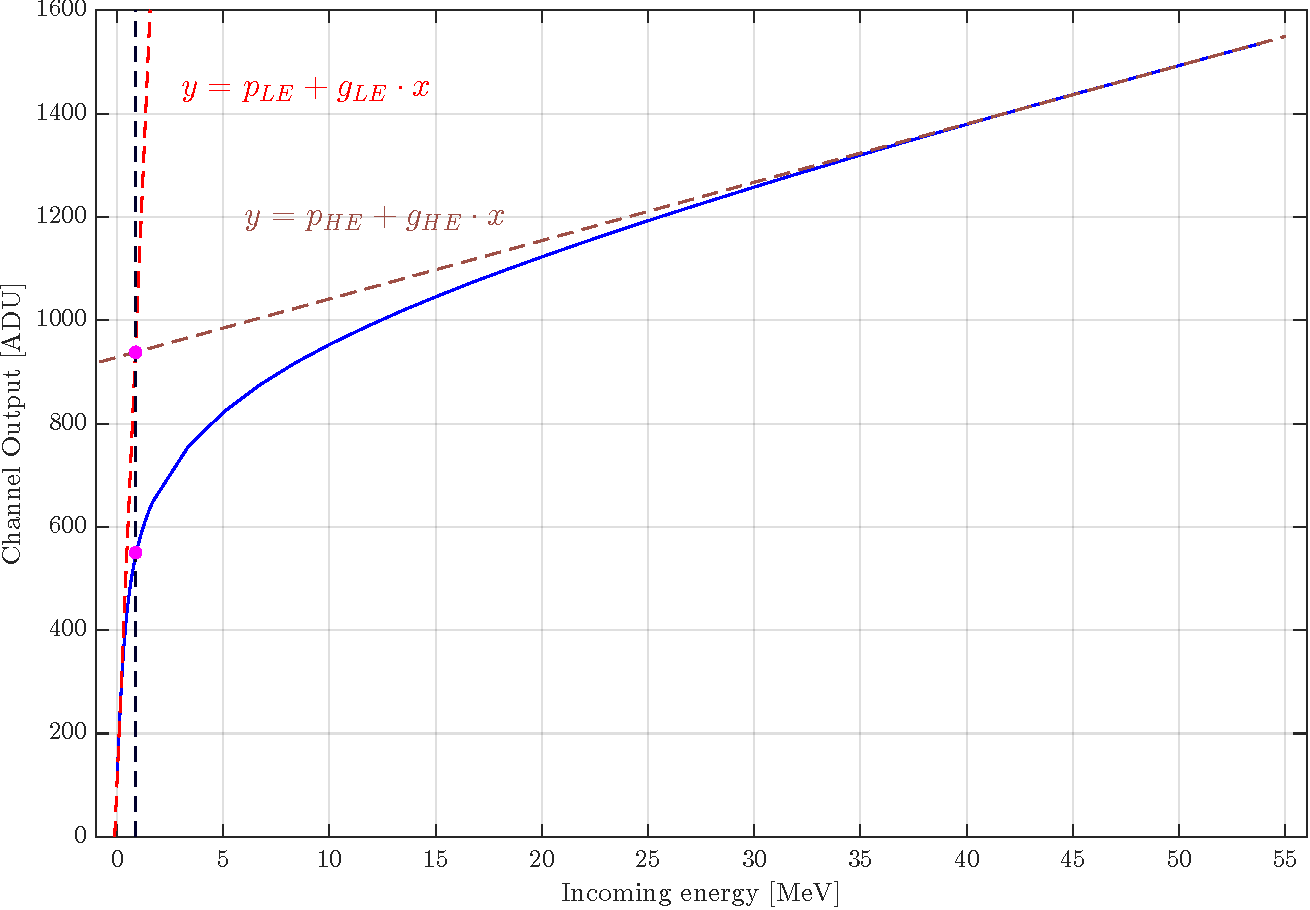
\includegraphics[width=0.65\textwidth]{Images/chap1/results/FDT/fdt_calcolo_kink.pdf}
    \caption{Method for determining the kink position: the linear models used to interpolate the transfer function in the low and high energy region are also reported.}
    \label{figFDTkinkVariation}
\end{figure}

\begin{figure}[h!]
    \centering
    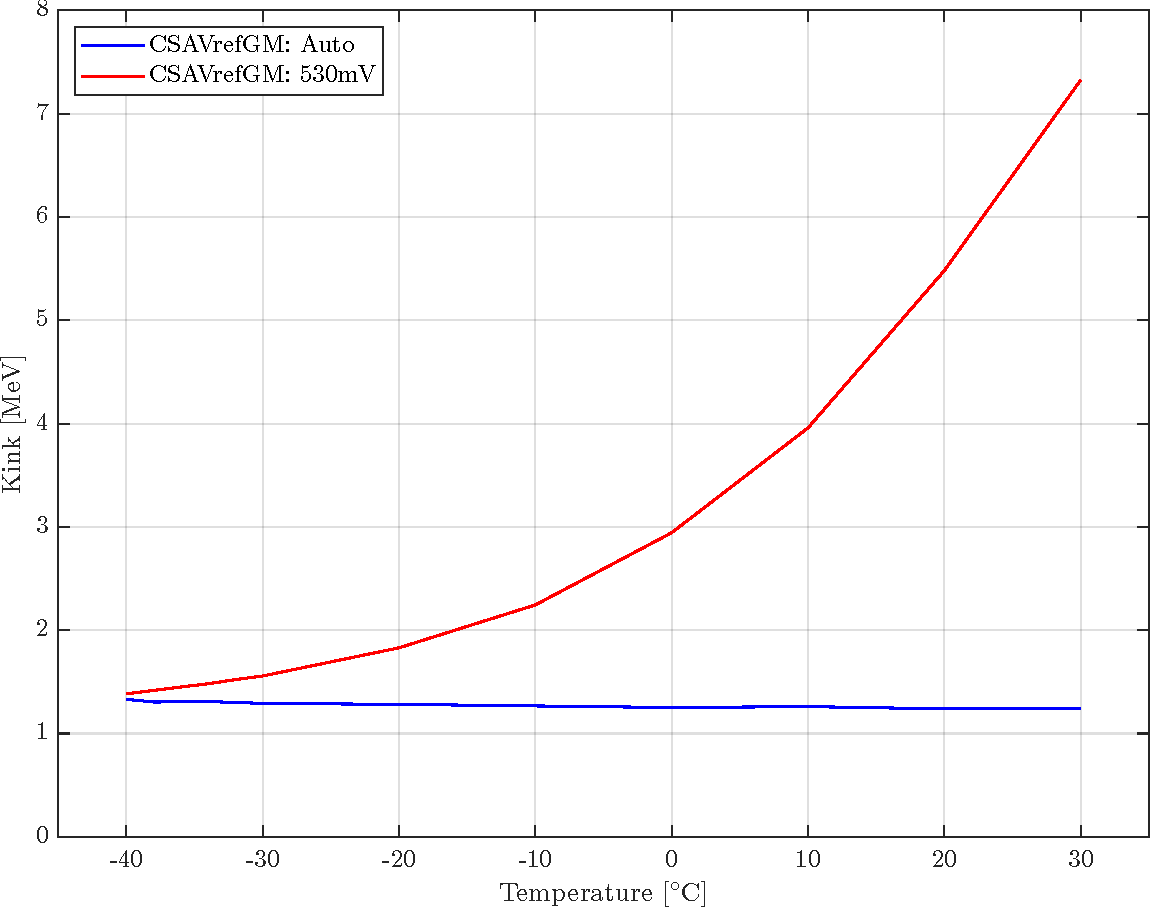
\includegraphics[width=0.55\textwidth]{Images/chap1/results/FDT/plot_pedestal_gain_auto_530mV.pdf}
    \caption{Kink behaviour as a function of temperature when \texttt{CSAVrefGM} is either fixed at \SI{530}{\milli\volt} (in red) or automatically varied as a function of temperature (in blue).}
    \label{figFDTkinkVariationResult}
\end{figure}

\par
It is easy to see that in the case where \texttt{CSAVrefGM} varies dynamically on the basis of temperature, the kink remains at an almost constant value, varying only \SI{6.95}{\percent} between \SI{-40}{\celsius} and \SI{30}{\celsius}. Conversely, in the case where this voltage is set at \SI{530}{\milli\volt} regardless of temperature, the kink undergoes a \SI{429}{\percent} variation between the two temperature extremes.


%-------------------------------------------------------------------------------
%	Global threshold voltage
%-------------------------------------------------------------------------------

\section{Global threshold voltage}
\label{thresholdVoltageANALYSIS}

This Section illustrates the measurements performed on the 8-bit DAC that provides two voltages $V_{\textit{tp}}$ and $V_{\textit{tn}}$ used by the threshold generator (described in \hyperref[secGAPSfrontend]{Appendix \ref{secGAPSfrontend}}) to generate the Signal-Over-Threshold (SOT) comparator voltage. In particular, the difference between the two voltages $\Delta V_{\textit{t}} = V_{\textit{tp}}-V_{\textit{tn}}$ is the meaningful quantity and will be referred to as \textit{global threshold voltage}: the higher $\Delta V_{\textit{t}}$, the higher the threshold of the SOT comparator. It has to be noted that the voltage $V_{\textit{tp}}$ remains constant by varying the DAC codes, whereas the voltage $V_{\textit{tn}}$ can vary from \SI{0}{\volt} to $(V_{\textit{tp}}+V_{\textit{s}})$, where $V_{\textit{s}}$ is a voltage margin which permits to obtain negative $\Delta V_{\textit{t}}$. 

\par
During design of this circuit, the DAC voltage Least Significant Bit (LSB) has been chosen to be \cite{sonzogni_2021_design}

\begin{equation}
    V_{\textit{tn, LSB}} = \SI{1.2}{\milli\volt}
\end{equation}

\noindent
Since the DAC bits are 8, the maximum value of the DAC codes is $2^{8}-1$. This forces the maximum value of $V_{\textit{tn}}$ to be

\begin{equation}
    V_{\textit{tn, max}} = V_{\textit{tn, lsb}} \cdot 255 = \SI{306}{\milli\volt}
\end{equation}

\begin{figure}[ht]
    \centering 
    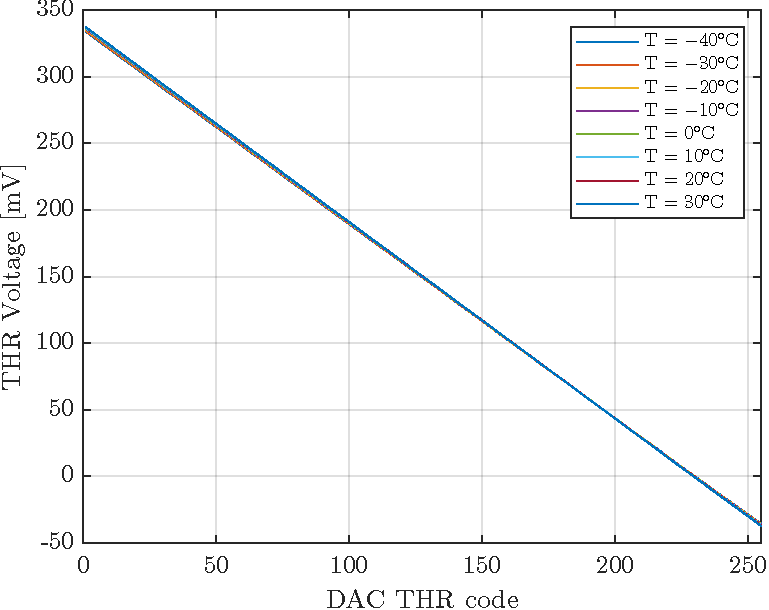
\includegraphics[width=0.63\textwidth]{Images/chap1/results/DAC_thr/DAC_thr_voltage_TEMP.pdf}
    \caption{$\Delta V_{\textit{t}}$ voltage with respect to DAC code varying temperature between \SI{-40}{\celsius} and \SI{30}{\celsius}.}
    \label{figDACthrtemp}
\end{figure}

\noindent
\hyperref[figDACthrtemp]{Figure \ref{figDACthrtemp}} shows the $\Delta V_{\textit{t}}$ voltage with respect to DAC codes varying from 0 to 255 measured at temperatures comprised between \SI{-40}{\celsius} and \SI{30}{\celsius} on channel 31. 

\hyperref[tabDACmaxlsb]{Table \ref{tabDACmaxlsb}} shows the maximum value assumed by $V_{\textit{tn}}$ and the corresponding DAC voltage LSB measured at each temperature.

\begin{table}[ht]
    \centering
    \begin{tabular}{c c c} 
        \Xhline{2\arrayrulewidth}
        Temperature [\SI{}{\celsius}] & $V_{\textit{tn, max}}$ [\SI{}{\milli\volt}] & $V_{\textit{tn, lsb}}$ [\SI{}{\milli\volt}] \T\B \\
        \hline
        -40 & 333.87 & 1.45 \T\B \\
        -30 & 334.32 & 1.45 \T\B \\
        -20 & 335.35 & 1.46 \T\B \\
        -10 & 335.91 & 1.46 \T\B \\
        0 & 336.46 & 1.46 \T\B \\
        10 & 336.78 & 1.46 \T\B \\
        20 & 337.15 & 1.47 \T\B \\
        30 & 337.26 & 1.47 \T\B \\
        \Xhline{2\arrayrulewidth}
    \end{tabular}
    \caption{$V_{\textit{tn, max}}$ and $V_{\textit{tn, lsb}}$ measured at temperatures ranging from \SI{-40}{\celsius} to \SI{30}{\celsius}.}
    \label{tabDACmaxlsb}
\end{table}

\par
Threshold voltage measurements have been evaluated by interpolating experimental results with the linear regression model shown in \hyperref[DAClinearmodel]{Equation (\ref{DAClinearmodel})}. Coefficient $a$ is expressed in \SI{}{\milli\volt} and coefficient $b$ in \SI{}{\milli\volt/\celsius}. The Root Mean Square Error (RMSE) is reported for each temperature.

\begin{equation}
    y = a + b \cdot x
\label{DAClinearmodel}
\end{equation}

\hyperref[tabDAClinearmodel1]{Table \ref{tabDAClinearmodel1}} offers a list of the model coefficients calculated over the threshold voltage measurements taken at temperatures spanning from \SI{-40}{\celsius} to \SI{30}{\celsius} along with the model RMSE.

\begin{table}[ht]
    \centering
    \begin{tabular}{c c c c} 
        \Xhline{2\arrayrulewidth}
        Temperature [\SI{}{\celsius}] & a [\SI{}{\milli\volt}] & b [\SI{}{\milli\volt/\celsius}] & RMSE \T\B \\
        \hline
        -40 & 335.12 & -1.46 & 0.15 \T\B \\
        -30 & 335.67 & -1.46 & 0.14 \T\B \\
        -20 & 336.58 & -1.46 & 0.13 \T\B \\
        -10 & 337.15 & -1.47 & 0.13 \T\B \\
        0 & 337.79 & -1.47 & 0.11 \T\B \\
        10 & 338.17 & -1.47 & 0.10 \T\B \\
        20 & 338.51 & -1.47 & 0.10 \T\B \\
        30 & 338.64 & -1.48 & 0.09 \T\B \\
        \Xhline{2\arrayrulewidth}
    \end{tabular}
    \caption{Linear regression model coefficients evaluated over global threshold measurements taken at temperatures varying from \SI{-40}{\celsius} to \SI{30}{\celsius}.}
    \label{tabDAClinearmodel1}
\end{table}

\par
\hyperref[figDACthrtemp4030]{Figure \ref{figDACthrtemp4030}} shows the global threshold voltage trend with respect to the DAC code for temperatures ranging from \SI{-40}{\celsius} to \SI{-30}{\celsius} and \SI{2}{\celsius} increments. As done previously, the global threshold voltage measurements have been evaluated by interpolating the same linear regression model described in \hyperref[DAClinearmodel]{Equation (\ref{DAClinearmodel})}. The model coefficients are proposed in \hyperref[tabDAClinearmodel2]{Table \ref{tabDAClinearmodel2}}. It is immediate to see that in the \SI{-40}{\celsius} to \SI{-30}{\celsius} temperature range, the slope, $b$, of the DAC trans-characteristic remains constant with respect to temperature, while the intercept, $a$, slightly increases with an increase of temperature.

\begin{figure}[h!]
    \centering
    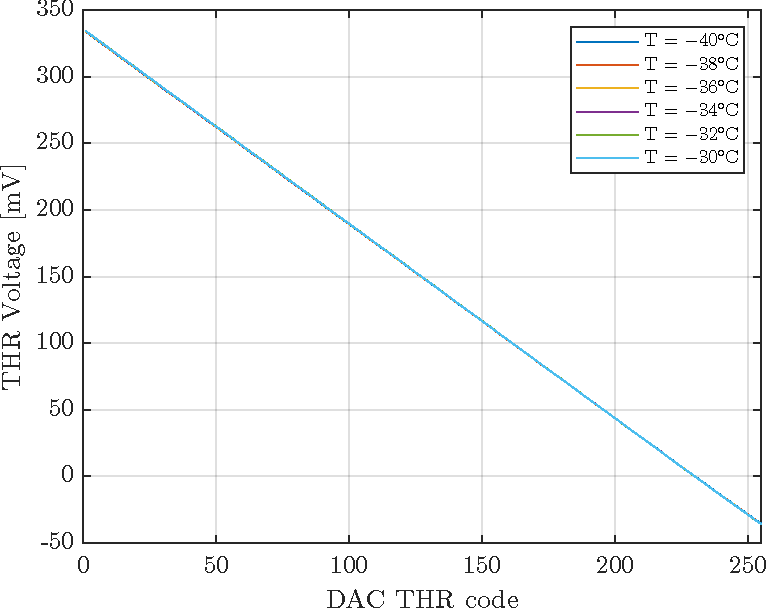
\includegraphics[width=0.63\textwidth]{Images/chap1/results/DAC_thr/DAC_thr_voltage_40-30.pdf}
    \caption{$\Delta V_{\textit{t}}$ voltage with respect to DAC code varying temperature between \SI{-40}{\celsius} and \SI{-30}{\celsius}.}
    \label{figDACthrtemp4030}
\end{figure}

\begin{table}[h!]
    \centering
    \begin{tabular}{c c c c} 
        \Xhline{2\arrayrulewidth}
        Temperature [\SI{}{\celsius}] & a [\SI{}{\milli\volt}] & b [\SI{}{\milli\volt/\celsius}] & RMSE \T\B \\
        \hline
        -40 & 335.12 & -1.46 & 0.15 \T\B \\
        -38 & 335.27 & -1.46 & 0.14 \T\B \\
        -36 & 335.50 & -1.46 & 0.14 \T\B \\
        -34 & 335.62 & -1.46 & 0.14 \T\B \\
        -32 & 335.74 & -1.46 & 0.13 \T\B \\
        -30 & 335.67 & -1.46 & 0.13 \T\B \\
        \Xhline{2\arrayrulewidth}
    \end{tabular}
    \caption{Linear regression model coefficients evaluated over global threshold measurements taken at temperatures varying from \SI{-40}{\celsius} to \SI{-30}{\celsius}.}
    \label{tabDAClinearmodel2}
\end{table}

\par
\hyperref[figDACfinethrtemp]{Figure \ref{figDACfinethrtemp}} presents the trend of the global threshold voltage with respect to the DAC code by varying the 3 bits fine threshold code on channel 31 at a constant temperature of \SI{-40}{\celsius}. As it can been appreciated in \hyperref[tabDAClinearmodel3]{Table \ref{tabDAClinearmodel3}}, the change in fine threshold code keeps the gradient unaltered while operating a shift in the DAC transfer function.

\begin{figure}[h!]
    \centering
    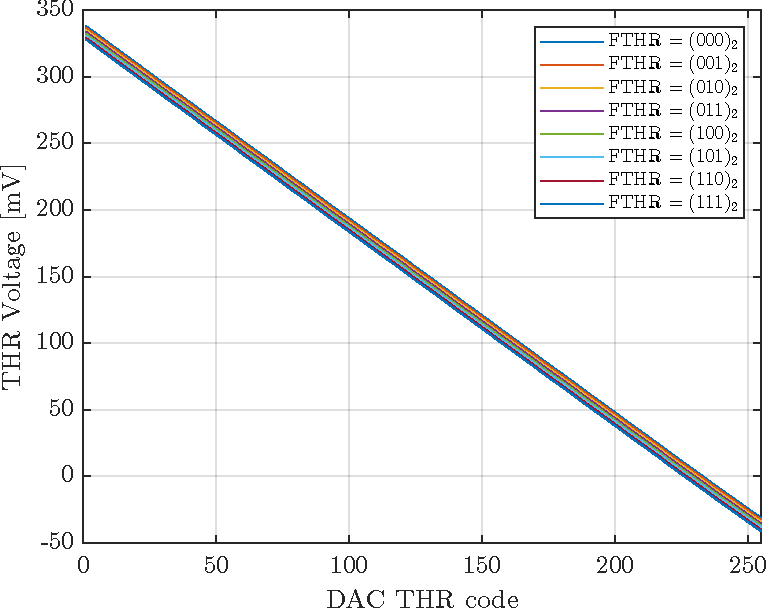
\includegraphics[width=0.63\textwidth]{Images/chap1/results/DAC_thr/DAC_thr_voltage_FTHR_-40C.pdf}
    \caption{$\Delta V_{\textit{t}}$ voltage with respect to DAC code and varying fine threshold (FTHR) code at \SI{-40}{\celsius}.}
    \label{figDACfinethrtemp}
\end{figure}

\begin{table}[h!]
    \centering
    \begin{tabular}{c c c c c} 
        \Xhline{2\arrayrulewidth}
        \multicolumn{2}{c}{FTHR} & a [\SI{}{\milli\volt}] & b [\SI{}{\milli\volt/bit}] & RMSE \T\B \\
        \hline
        0 & $(000)_{2}$ & 339.49 & -1.46 & 0.155 \T\B \\
        1 & $(001)_{2}$ & 338.10 & -1.46 & 0.152 \T\B \\
        2 & $(010)_{2}$ & 336.52 & -1.46 & 0.155 \T\B \\
        3 & $(011)_{2}$ & 335.12 & -1.46 & 0.154 \T\B \\
        4 & $(100)_{2}$ & 333.71 & -1.46 & 0.160 \T\B \\
        5 & $(101)_{2}$ & 332.22 & -1.46 & 0.156 \T\B \\
        6 & $(110)_{2}$ & 330.64 & -1.46 & 0.152 \T\B \\
        7 & $(111)_{2}$ & 329.29 & -1.46 & 0.154 \T\B \\
        \Xhline{2\arrayrulewidth}
    \end{tabular}
    \caption{Linear regression model coefficients evaluated over global threshold measurements taken by spanning the 8-bit DAC code and by varying the fine threshold (FTHR) code.}
    \label{tabDAClinearmodel3}
\end{table}


%-------------------------------------------------------------------------------
%	Equivalent Noise Charge (ENC) at -40 °C
%-------------------------------------------------------------------------------

\section{Equivalent Noise Charge (ENC) at \SI{-40}{\celsius}} \label{ENC} % -40$^{\circ}$C
The measurement of the Equivalent Noise Charge (ENC) is of fundamental importance to evaluate the performance of the channel in terms of resolution and, therefore, of minimum detectable energy. The ENC represents the electronic noise generated by the front-end channel reported in the form of equivalent noise charge at the channel input. In the case of GAPS, the main requirement for the channel comes from the resolution, that must be less than \SI{4}{\kilo\electronvolt}: this is equivalent to saying that the ENC (FWHM) for each channel must be less than \SI{4}{\kilo\electronvolt} in order to consider the channel suitable for the experiment.

\par
ENC is calculated by dividing the standard deviation of the noise, obtained from the pedestal measurement in ADU, by the low energy gain of the channel transfer function, extracted from the input-output characteristic measurements and expressed in (ADU)/(DAC injection units):

\begin{equation}
    ENC = \frac{\sigma_{\textit{ped}} \cdot 2.35}{\mu_{\textit{ch}}} \cdot \SI{0.841}{\frac{\SI{}{\kilo\electronvolt}}{\SI{}{DAC\_inju}}} 
\end{equation}

\noindent
where $\sigma_{\textit{ped}}$ is the channel noise standard deviation and $\mu_{\textit{ch}}$ is the channel low energy gain. The \SI{0.841}{\frac{\SI{}{\kilo\electronvolt}}{\SI{}{DAC\_inju}}} value represents a conversion factor for obtaining the \SI{}{\kilo\electronvolt} measurements and it is calculated as follows:

\begin{equation}
    C_{\textit{inj}} \cdot \frac{V_{\textit{LSB, CAL}}}{\SI{0.044}{\frac{fC}{\kilo\electronvolt}}} = \SI{1.184}{\pico\farad} \cdot \frac{\SI{31.25}{\frac{\micro\volt}{DAC\_inju}}}{\SI{0.044}{\frac{fC}{\kilo\electronvolt}}} = \SI{0.841}{\frac{\kilo\electronvolt}{DAC\_inju}}
    \label{eqConversionFactor}
\end{equation}

\noindent
where $C_{\textit{inj}}$ is the injection capacitance, $V_{\textit{LSB, CAL}}$ is the LSB value of the 16-bit calibration DAC and \SI{0.044}{\frac{fC}{\kilo\electronvolt}} is the conversion factor between \SI{}{fC} and \SI{}{\kilo\electronvolt}.

\par
Lastly, 2.35 is the \textit{Fano factor}. This factor is taken into account since the ENC measurement must be expressed at Full Width at Half Maximum (FWHM). One does not simply want to consider the standard deviation of the pedestal, but the width of its Gaussian distribution at half of its maximum height. To obtain this measurement, the standard deviation of the pedestal must be multiplied by the Fano factor.

\par
\hyperref[figENCnormal]{Figure \ref{figENCnormal}} represents the ENC FWHM with and without $\SI{40}{\pico\farad}$ detector capacitors, that have been soldered on the test board and connected to the first 8 (0 to 7) channels of the ASIC in order to emulate the Si(Li) detectors capacitance. It is clear to see from the graph on the right that channels with the capacitors installed experience an increase in ENC, as it should be expected \cite{iakovidis_2018_vmm}.

\begin{figure}[ht]
    \centering
    \begin{tabular}{cc}
         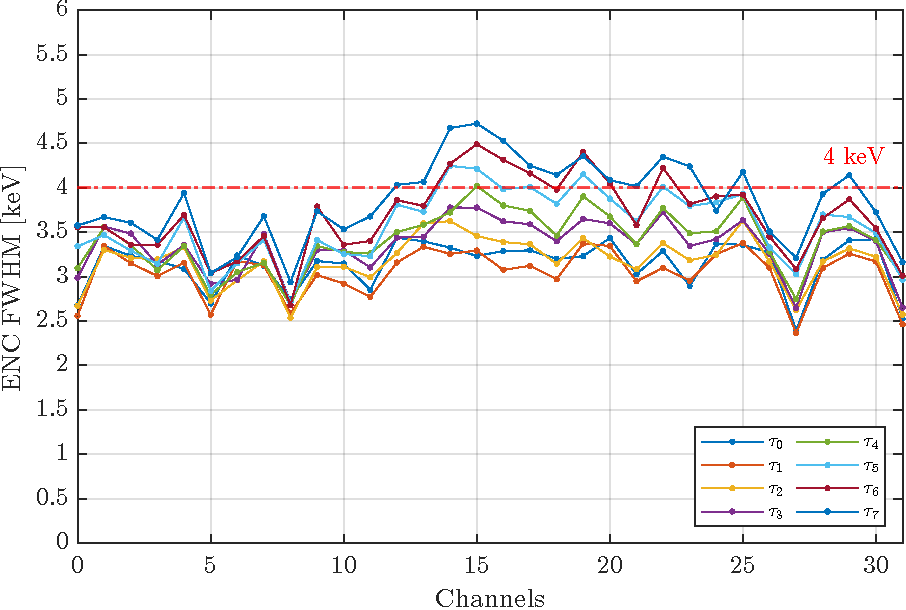
\includegraphics[width=0.475\textwidth]{Images/chap1/results/ENC_minus40C/ASIC_cold_wocaps_normal.pdf} &  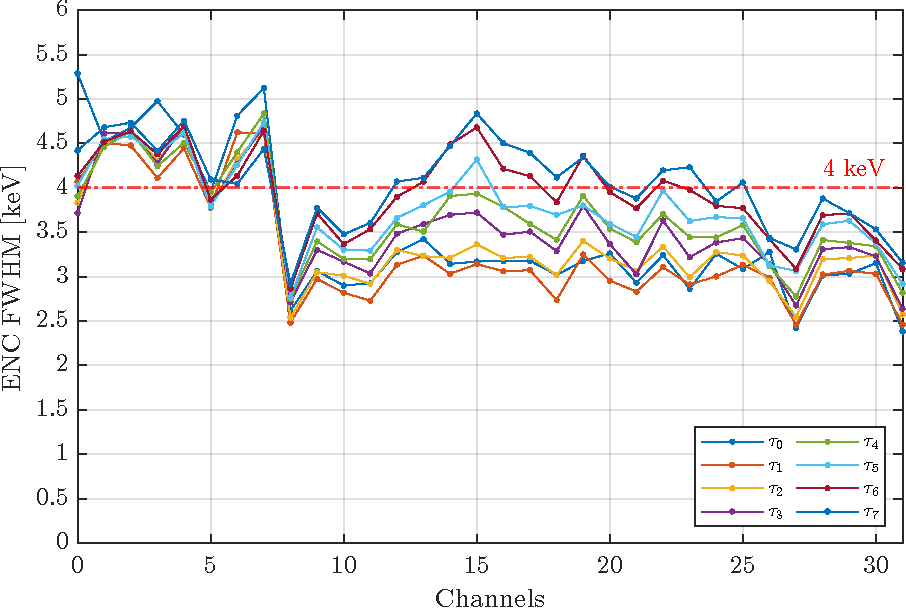
\includegraphics[width=0.475\textwidth]{Images/chap1/results/ENC_minus40C/ASIC_cold_wcaps_normal.pdf} \\
    \end{tabular}
    \caption{Graphs showing ENC FWHM without detector capacitors (on the left) and with detector capacitors (on the right) at \SI{-40}{\celsius} without removal of external interference.}
    \label{figENCnormal}
\end{figure}

\par
Since the ENC is a measurement derived from the pedestal, it is also subject to interference phenomena arising from electromagnetic noise present in the environment where the tests are performed. In this regard, a method was devised to remove interference contributions not directly attributable to pure electronic noise and the results of the analysis are presented in the following Sections.

\subsection{Sampled pedestal processing}
The pedestal is simultaneously dependent on both the channel on which the measurement is made, $y$, and the specific sample taken from the measurement, $x$, as the sum of 3 components. The first component, $p_0[y]$, represents the ideal pedestal free of external noise and interference, which therefore only depends on the specific channel on which the measurement is made. The second component, $n[x, y]$, represents the stochastic noise and the third one represents the deterministic interference component, $d[x]$. In this first analysis, the deterministic component, $d[x]$, is assumed to be common to all channels and therefore it only depends on the specific sample. For this reason, the pedestal can be written as

\begin{equation} \label{eq1}
    p[x,y] = p_0[y] + n[x, y] + d[x]
\end{equation}

\noindent
where
\begin{itemize}
    \itemsep0em 
    \item $x=1,2,...,1000$ represents the sample number.
    \item $y=0,1,...,31$ represents the channel number.
    \item $p_0$ is the ideal pedestal without noise and external interference and depends on $y$ only.
    \item $n$ is the stochastic noise component of the pedestal.
    \item $d$ is the deterministic external interference, at first we assume that it is common to all channels and it depends on $x$ only.
\end{itemize}

\subsection{Evaluation of deterministic interference}
For every sample $x$ we evaluate the mean value $p_{m}$ of the 32 channels sampled pedestal

\begin{equation} \label{eq2}
    \begin{split}
        p_m[x] & = \frac{1}{32} \sum_{y=0}^{31} p[x,y] \\
        & = \frac{1}{32} \sum_{y=0}^{31} (p_0[y] + n[x, y] + d[x]) \\
        & = p_{m, 0} + d[x]
    \end{split}
\end{equation}

\noindent
where

\begin{equation}
     \frac{1}{32} \sum_{y=0}^{31} p_0[y] = p_{m, 0}
\end{equation}

\noindent
it is due to the fact that the ideal pedestal depends entirely on the specific channel on which it is measured, so averaging the ideal pedestal over all 32 channels provides a channel-independent global average, representing the common contribution of all channels. On the other hand, it is possible to say that

\begin{equation}
     \frac{1}{32} \sum_{y=0}^{31} n[x,y] \simeq 0
\end{equation}

\noindent
and it comes from the stochastic nature of the noise, which has a constant power spectral density with respect to frequencies. This means that each frequency has the same contribution to the overall noise, thus resulting in an approximately zero average.

\par
Assuming in this first discussion that the interference contribution is common to all channels, it is easy to state that averaging the external interference $d[x]$ over the 32 channels returns the interference itself, the latter acting with the same proportion on all channels.

\begin{equation}
     \frac{1}{32} \sum_{y=0}^{31} d[x] = d[x]
\end{equation}

\subsection{Pedestal without external interference}

For every $x$ the evaluated interference is subtracted from the samples pedestal:

\begin{equation}
    \begin{split}
        p'[x,y] & = p[x,y] - p_m[x] \\
        & = p_0[y] + n[x,y] + \cancel{d[x]} - p_{m_0} - \cancel{d[x]} \\
        & = p_0[y] - p_{m_0} + n[x,y]
    \end{split}
\end{equation}

\noindent
The standard deviation with respect to $x$ of this new pedestal depends on the stochastic noise $n$ only.

\begin{figure}[h!]
    \centering
    \begin{tabular}{cc}
         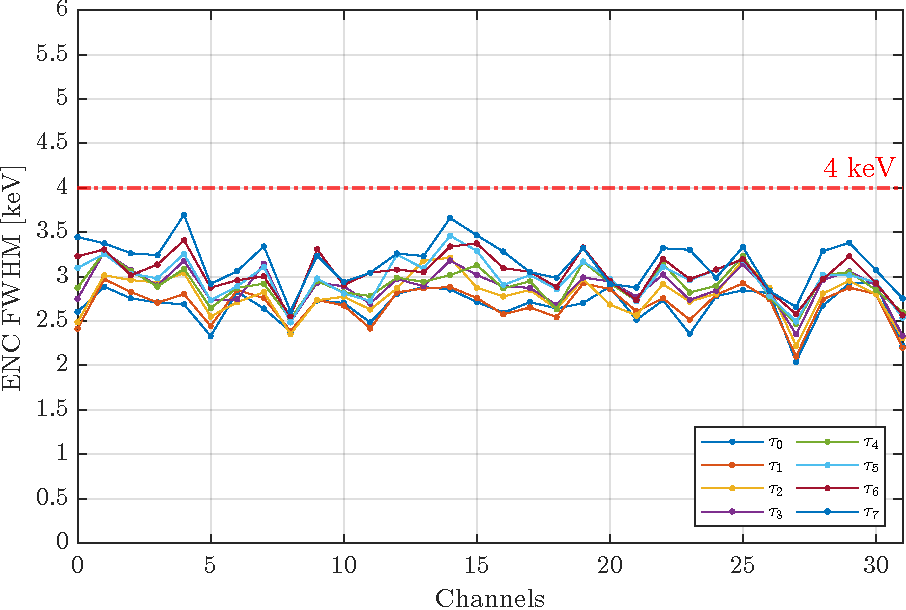
\includegraphics[width=0.475\textwidth]{Images/chap1/results/ENC_minus40C/ASIC_cold_wocaps_wo_mean.pdf} &  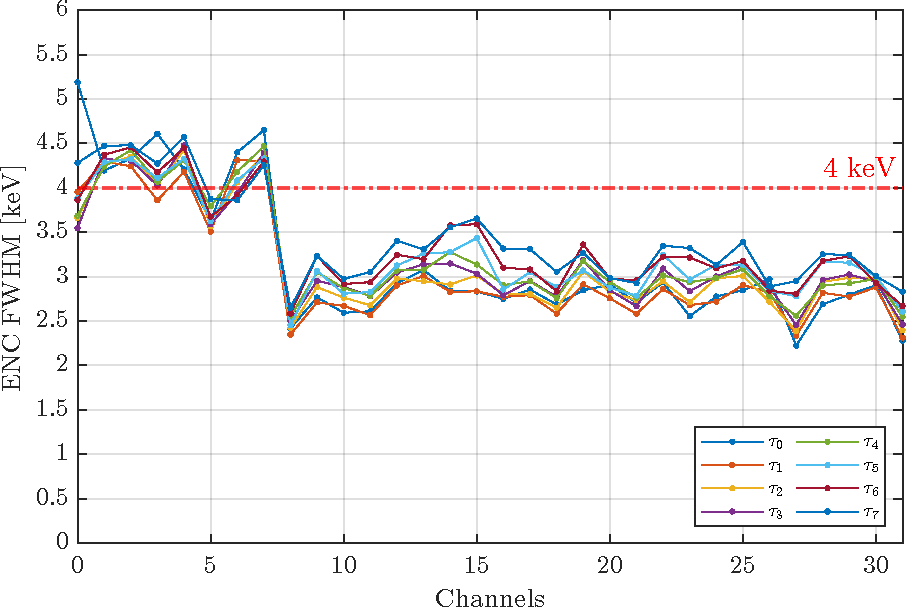
\includegraphics[width=0.475\textwidth]{Images/chap1/results/ENC_minus40C/ASIC_cold_wcaps_wo_mean.pdf} \\
    \end{tabular}
    \caption{Graphs showing ENC FWHM without detector capacitors (on the left) and with detector capacitors (on the right) at \SI{-40}{\celsius} without external interference.}
    \label{figENCwomean}
\end{figure}

\noindent
With this first method, it is therefore possible to remove the constant deterministic interference contribution, assuming to a first approximation that the disturbance acts uniformly on all 32 channels. \hyperref[figENCwomean]{Figure \ref{figENCwomean}} shows the result of the application of this first algorithm on the data shown in figure \hyperref[figENCnormal]{Figure \ref{figENCnormal}}. It is possible to appreciate the reduction of ENC, which is free of the deterministic interference component.

\subsection{Weighted external interference}
The method illustrated in this Section interprets the contribution of external deterministic interference as channel-specific, making the disturbance channel-dependent by means of a weighting factor that determines its impact, more or less marked, on the specific channel. If we assume that the same external interference $d[x]$ affects each channel with a different weight, \hyperref[eq1]{Equation (\ref{eq1})} changes as follows

\begin{equation} \label{eq3}
    p[x,y] = p_0[y] + n[x,y] + k[y] \cdot d[x]
\end{equation}

\noindent
It can be seen that the pedestal is still represented as a sum of 3 contributions, but in this case the deterministic component is weighted by means of a weight factor that determines how much the deterministic disturbance impacts on the specific channel. It goes without saying that for this method to be effective, the sample size must be sufficiently high in order to guarantee sufficiently comprehensive statistics for each individual channel. \hyperref[eq2]{Equation (\ref{eq2})} becomes

\begin{equation} \label{eq4}
    p_m[x] = p_{m_0} + k_m \cdot d[x]
\end{equation}

\noindent
where $k_m$ is the average over the 32 channels of the weight factor and can be represented as a constant factor common to all channels.

\begin{equation}
    \frac{1}{32} \sum_{y=0}^{31} k[y] \cdot d[x] = k_m \cdot d[x]
\end{equation}

\noindent
From \hyperref[eq3]{Equation (\ref{eq3})} we derive that

\begin{equation}
    d[x] = \frac{1}{k[y]} (p[x,y] - p_0[y] - n[x,y])
\end{equation}

\noindent
and therefore by replacing $d[x]$ in \hyperref[eq4]{Equation (\ref{eq4})} we obtain

\begin{equation}
    \begin{split}
        p_m[x] & = p_{m_0} + \frac{k_m}{k[y]}(p[x,y] - p_0[y] - n[x,y]) \\
        & = p_{m_0} - \frac{k_m}{k[y]} p_0[y] + \frac{k_m}{k[y]} (p[x,y] - n[x,y])
    \end{split}
\end{equation}

\noindent
By plotting $p_m[x]$ as a function of $p[x,y]$ for a given channel and by interpolating it via a linear function, the slope $m$ of the interpolating function provides the ratio between the mean channel weight $k_m$ and the weight $k[y]$ of channel $y$

\begin{equation}
    m = \frac{k_m}{k[y]}
\end{equation}

\subsection{Pedestal without weighed external interference}
As done previously, it is now necessary to remove the contribution of external deterministic interference. For this reason, for a given channel $y$ and for every sample $x$ we evaluate

\begin{equation}
    \begin{split}
        p'[x,y] & = p[x,y] - \frac{1}{m} p_m[x] \\
        & = p_0[y] + n[x,y] + k[y] \cdot d[x] - \frac{k[y]}{k_m} (p_{m_0} + k_m \cdot d[x]) \\
        & = p_0[y] + n[x,y] - \frac{k[y]}{k_m} p_{m_0} + k[y] \cdot d[x] - \frac{k[y]}{\cancel{k[m]}} \cdot \cancel{k[m]} \cdot d[x] \\
        & = p_0[y] + n[x,y] - \frac{k[y]}{k_m} p_{m_0} + \cancel{k[y] \cdot d[x]} - \cancel{k[y] \cdot d[x]} \\
        & = p_0[y] - \frac{k[y]}{k_m} \cdot p_{m_0} + n[x,y]
    \end{split}
\end{equation}

\noindent
This results in the removal of the deterministic interference component from the Equation of the pedestal of each channel, reducing it entirely to the ideal contribution to which the purely stochastic component is added. Therefore, the distribution of $p'[x,y]$ depends only on the stochastic noise $n[x,y]$ for a given channel $y$.

\par
The result of the application of the latter method can be seen in \hyperref[figENCwofit]{Figure \ref{figENCwofit}}. It should be noted that, due to the limited sample size that characterises the dataset acquired during the measurements, this method is unable to provide an effective removal of the disturbance component, even resulting in a higher ENC contribution with respect to the initial one.

\begin{figure}[h!]
    \centering
    \begin{tabular}{cc}
         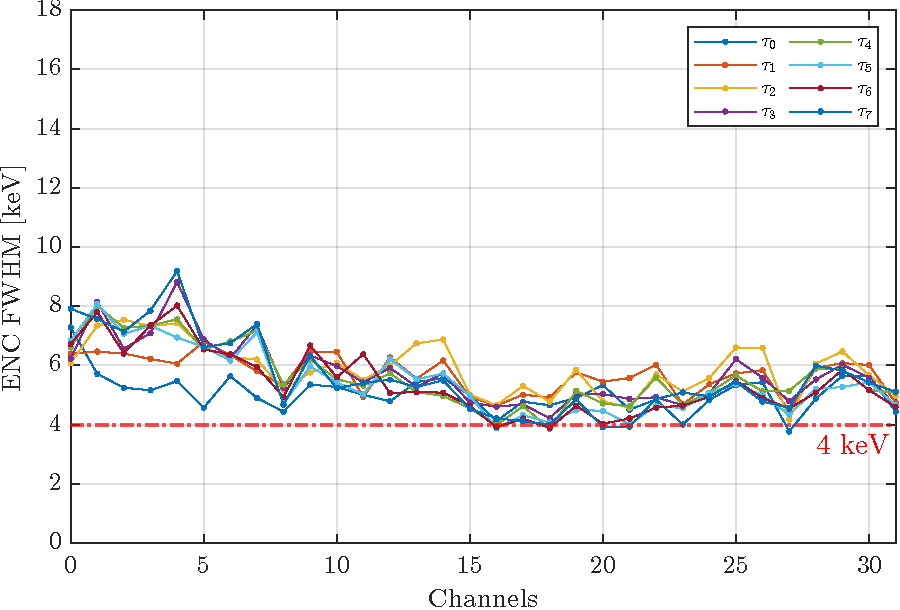
\includegraphics[width=0.475\textwidth]{Images/chap1/results/ENC_minus40C/ASIC_cold_wocaps_wo_fit.pdf} &  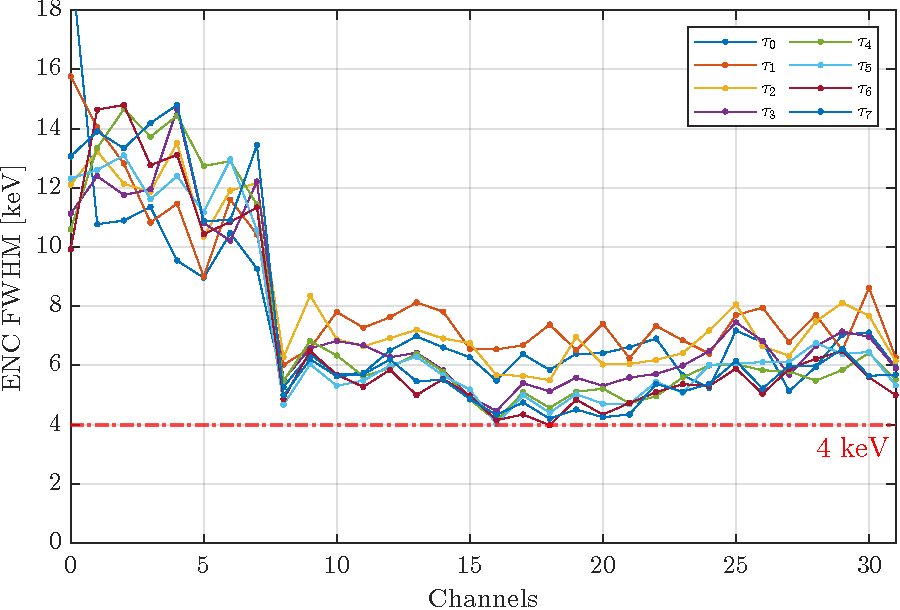
\includegraphics[width=0.475\textwidth]{Images/chap1/results/ENC_minus40C/ASIC_cold_wcaps_wo_fit.pdf} \\
    \end{tabular}
    \caption{Graphs showing ENC FWHM without detector capacitors (on the left) and with detector capacitors (on the right) at \SI{-40}{\celsius} without weighed external interference.}
    \label{figENCwofit}
\end{figure}
\chapter[Si(Li) tracker flight components validation]{Si(Li) tracker flight components \\validation} \label{ch2}

This Chapter provides a detailed description of the test setup and the test procedures followed to validated the flight items that will be used for the final assembly of the Si(Li) tracker of the GAPS detector. For each of the flight items, a report has been produced in order to detail all the most important parameters with their measured values. Every component has also been uniquely numbered following a specific alphanumeric pattern that can briefly sum up its most relevant characteristics, allowing it to be immediately recognised during the assembly process. This Chapter also provides a deep explanation of the results obtained during the testing activity on all the flight components.

\par
Tests were conducted in order to verify the integrity and proper functioning of the following items:

\begin{enumerate}
    %\bfseries
    \itemsep0em 
    \item Front-End Board (FEB).
    \item Dummy-1 front-end board.
    \item Flex-rigid board.
    \item Connector for termination.
    \item Front-end board shield.
\end{enumerate}

\par
The following Sections are structured as follows: First, the test setup used to verify the correct functioning of the component will be described and a description of the tests performed will be provided, then the results of the tests performed will be reported. 


\hyperref[figFlowChart]{Figure \ref{figFlowChart}} shows the flowchart associated with the testing and validation process of all flight items.

\begin{figure}[h!]
    \centering
    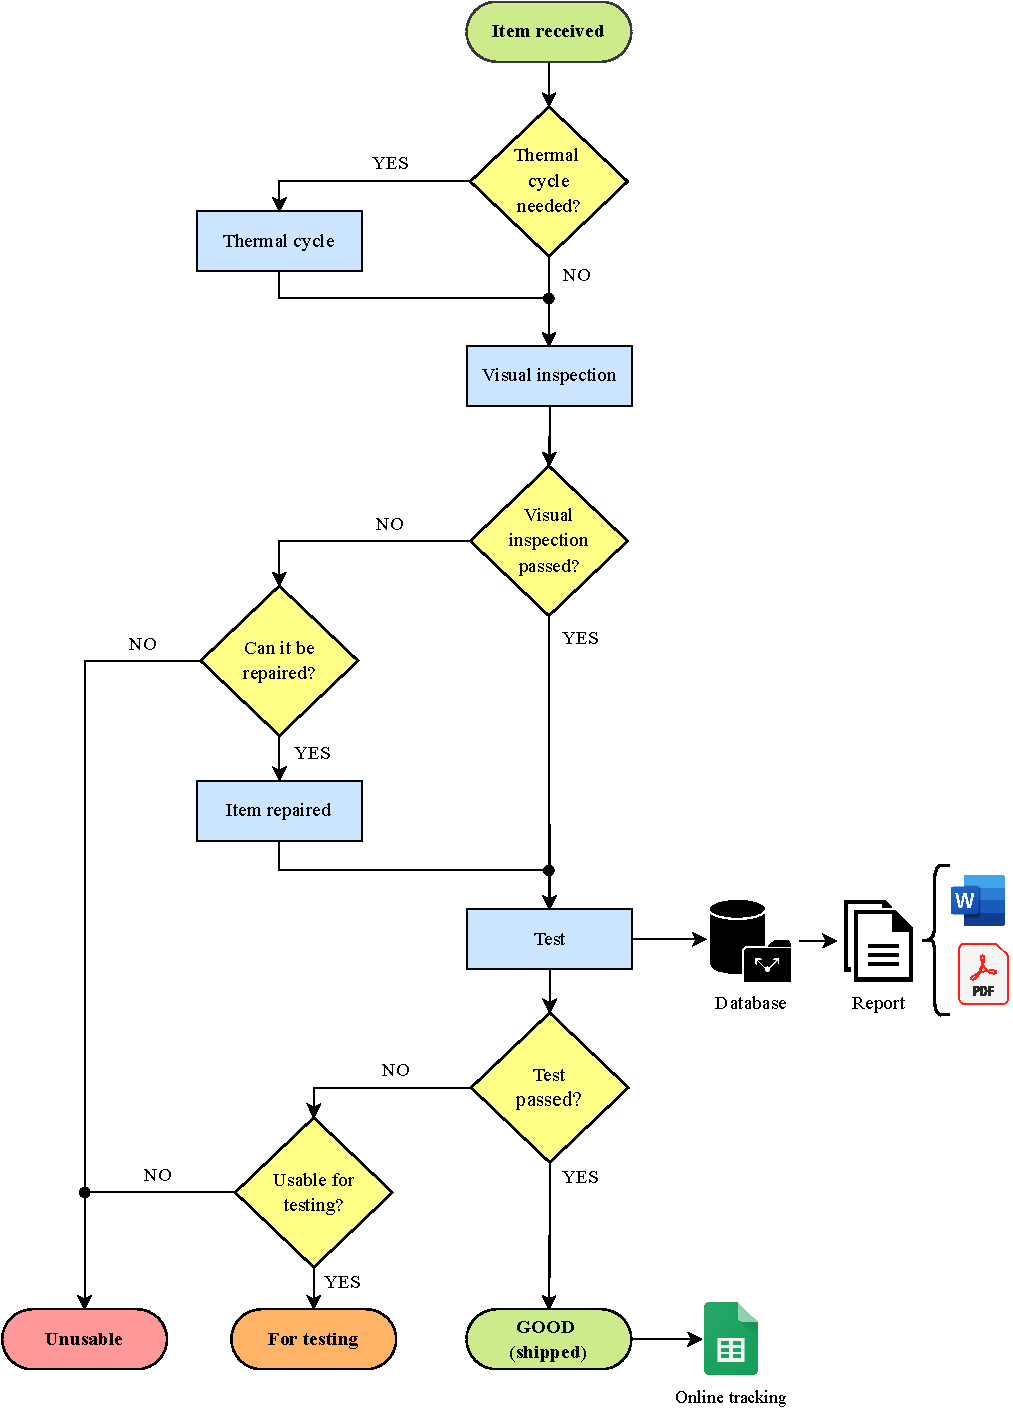
\includegraphics[width=0.8\textwidth]{Images/chap2/flight_item_validation_procedure.drawio.pdf}
    \caption{Flight item validation procedure flowchart.}
    \label{figFlowChart}
\end{figure}

At the end of the test procedure, test results are saved in a database and an item report is generated. Depending on the outcome of the tests performed, the item is classified as:

\begin{itemize}
    \item \textbf{GOOD}, meaning it passed all tests and can be used for tracker assembly.
    \item \textbf{USABLE for testing activity only}, if the component had a defect that was repaired.
    \item \textbf{UNUSABLE}, in case the component had a defect that could not be repaired.
\end{itemize}

\par
\noindent
The items classified as \textbf{GOOD} have been shipped to \textit{Columbia University} to be integrated into the experiment assembly process.


%-------------------------------------------------------------------------------
%   front-end board
%-------------------------------------------------------------------------------

\section{Front-End Board (FEB)} \label{sec21}

\par
The Front-End Board (FEB) that houses the SLIDER32 ASIC is shown in \mbox{\hyperref[figFEBimage]{Figure \ref{figFEBimage}}}. The board was designed in a cross-like shape to make room for the four Si(Li) detectors which will be wire-bonded to the ASIC through the smooth vertical tracks running in the central section of the FEB.

\begin{figure}[ht]
    \centering
    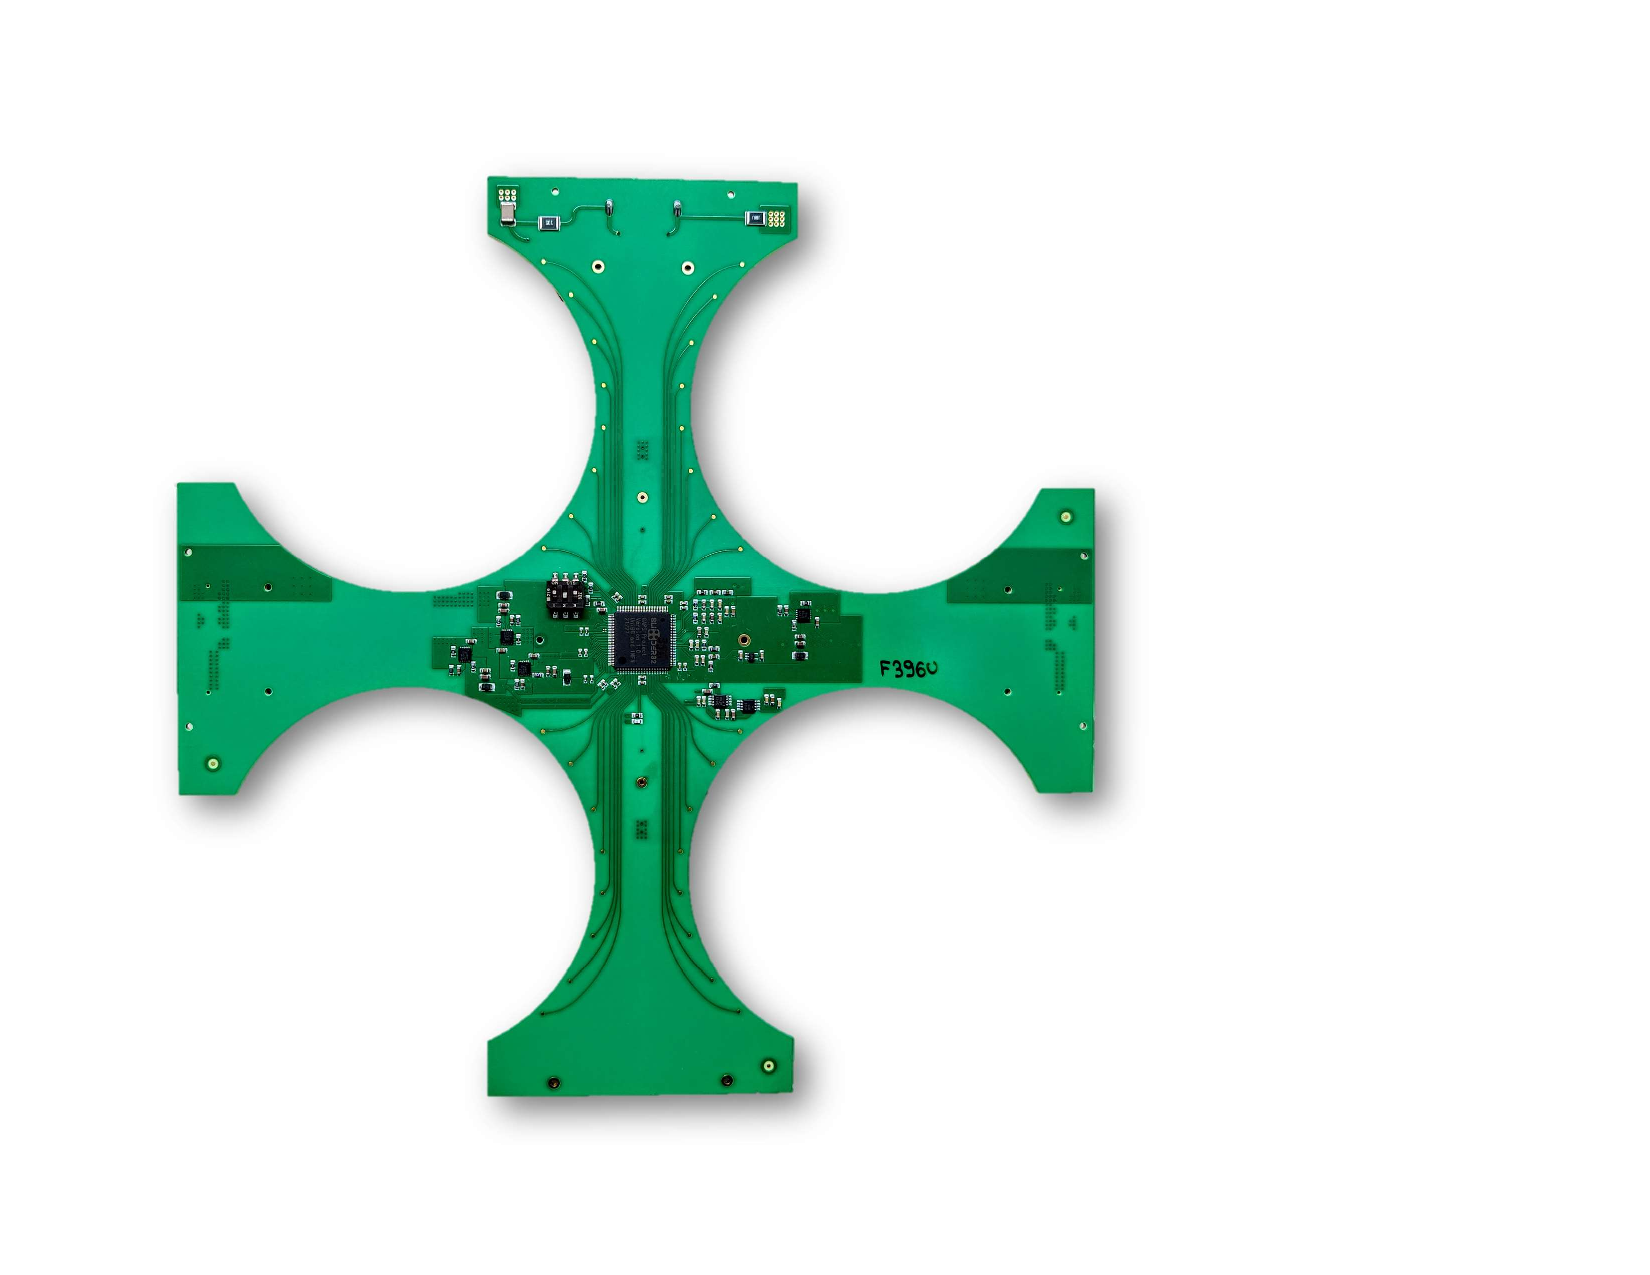
\includegraphics[width=0.7\textwidth]{Images/chap2/FEB_immagine.pdf}
    \caption{SLIDER32 front-end board No. \texttt{F396U} (US production).}
    \label{figFEBimage}
\end{figure}

\par
Each FEB houses the components necessary for the operation of the ASIC and Si(Li) sensors, including the power supplies, divided into High Voltage Power Supply (HVPS) required for the four detectors, and Low Voltage Power Supply (LVPS) necessary for the polarisation of the ASIC and its internal components. Each FEB is also equipped with a current reference for the Charge Sensitive Amplifier (CSA) input transistor, pull-up and pull-down resistors used in the transmission of the control signals, a 3-bit switch to set the address of the FEB, a 16-bit DAC for calibration and a temperature sensor. Within the tracker of the GAPS experiment, the FEBs will be connected to each other via an ERNI connector and a flex-rigid board, later described in \hyperref[flexrigids]{Section \ref{flexrigids}}. Each FEB is equipped with a male (model \texttt{254877}) and female (model \texttt{354178}) ERNI high-speed micro connectors, one used to connect the front-end board to the previous one and the other used to connect it to the following FEB.

\par

\par
The test of the front-end boards has been performed at ambient temperature and was aimed at verifying the proper functioning of the board and at looking for damages to the board or improperly soldered components, including the aforementioned ERNI connectors. The test has been performed in a twofold way:

\begin{itemize}
    \itemsep0em 
    \item By measuring the DC operating point of the ASIC with a Fluke 79 III digital multimeter and a Keysight N6705C DC Power analyser (with N6762A and N6733B modules installed);
    \item By running a purposely developed automated validation test controlled by a terasIC OpenVino Toolkit based on an ALTERA Cyclone V Field Programmable Gate Array (FPGA) board. This procedure performs several types of tests, which are summarised in the following list:
    
    \begin{enumerate}
        %\bfseries
        \itemsep0em 
        \item Noise (ENC).
        \item Pedestal.
        \item Self trigger.
        \item Threshold scan.
        \item Channel input-output characteristic.
        \item Waveform scan.
    \end{enumerate}
\end{itemize}

\par
A detailed representation of the setup used for the tests is reported in \hyperref[figFEBtest1]{Figure \ref{figFEBtest1}} and in \hyperref[figFEBtest2]{Figure \ref{figFEBtest2}}. At first, the setup depicted in \hyperref[figFEBtest1]{Figure \ref{figFEBtest1}} has been used. After having realised that with this configuration the proper soldering of the ERNI output connector could not be verified, the setup has been improved by including a second front-end board connected in series with the first one via a flex-rigid board as shown in \hyperref[figFEBtest2]{Figure \ref{figFEBtest2}}. This allowed to implement a communication test between the FEB under test and the FEB in series, thus verifying the correct functioning of the ERNI connector lodging the flex-rigid board connecting one FEB and the following. Specifically, the second version of the setup used is comprised of the following items:

\begin{figure}[h!]
    \centering
    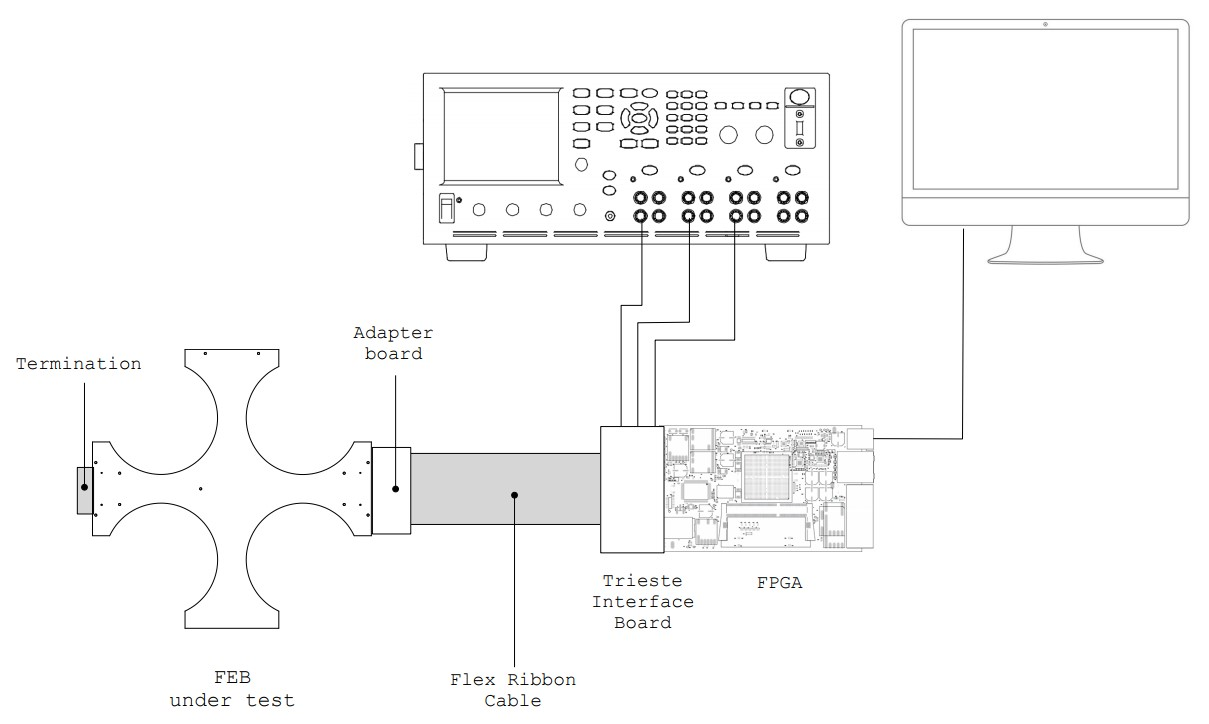
\includegraphics[width=0.95\textwidth]{Images/chap2/test_setup_FEB_1.jpg}
    \caption{Depiction of the setup adopted for the tests on the first set of FEBs.}
    \label{figFEBtest1}
\end{figure}

\begin{figure}[h!]
    \centering
    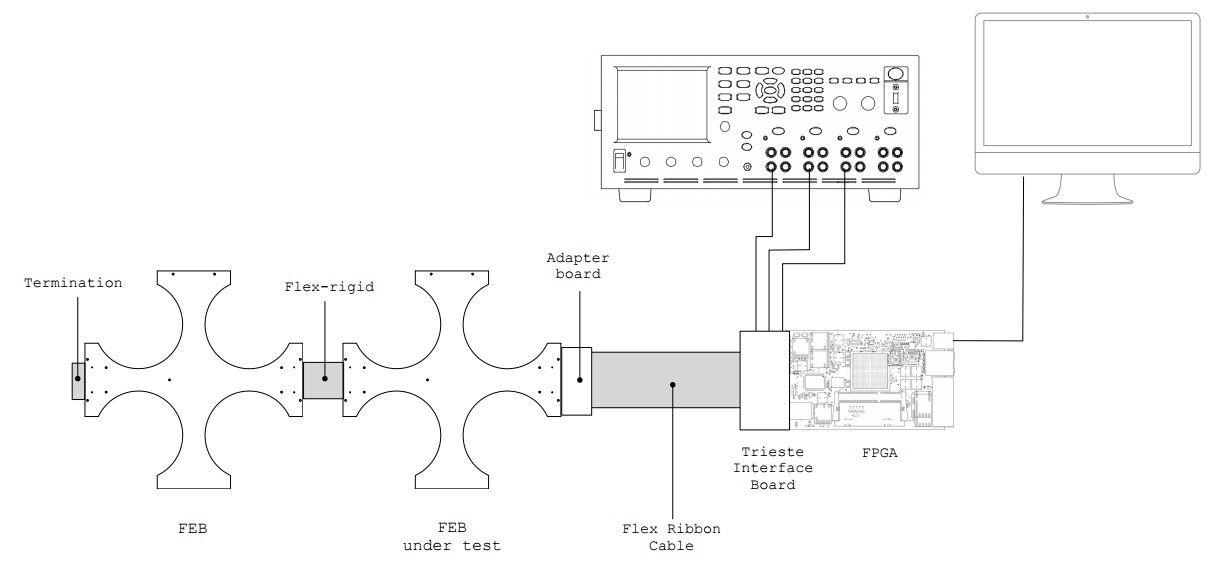
\includegraphics[width=0.95\textwidth]{Images/chap2/test_setup_FEB_2.jpg}
    \caption{Depiction of the improved setup adopted for the tests of the FEBs.}
    \label{figFEBtest2}
\end{figure}

\begin{itemize}
    \itemsep0em 
    \item Two front-end boards, each of which has a SLIDER32 ASIC onboard, as described in \hyperref[secGAPSfrontend]{Appendix \ref{secGAPSfrontend}}.
    \item A flex-rigid board, later described in \hyperref[flexrigids]{Section \ref{flexrigids}}, connecting the two FEBs.
    \item A Keysight N6705C DC Power analyser providing both analog and digital supply voltages to the FEB, with the same configuration as the one already discussed in \mbox{\hyperref[testboardsetup]{Section \ref{testboardsetup}}}.
    \item A flex ribbon cable connecting the interface board to the main test board.
    \item An adapter board connecting the FEB trough its female ERNI connector (model \texttt{354178}) to the flex ribbon cable.
    \item An ALTERA Cyclone V Field Programmable Gate Array (FPGA) programmed using Verilog, an Hardware Description Language (HDL) that allows to describe digital electronic systems. The FPGA sends Serial Peripheral Interface (SPI) commands to the FEB according to those expected by the ASIC digital back-end, listed in \hyperref[tabSPIcommand]{Table \ref{tabSPIcommand}}, that are propagated through all the connected FEBs by means of the flex-rigid boards.
    \item An interface board specifically designed to route the power supplies and the signals trough the flex ribbon cable to the front-end board under test.
    \item A PC running a Python-based testing program called \texttt{GAPS\_ModuleTester}, currently in its 4th version, connected to the FPGA via two Universal Serial Bus (USB) cables. This software has been specifically developed to perform a series of tests on the SLIDER32 ASIC and it is later described in \hyperref[sec21]{Section \ref{sec21}}.
\end{itemize}

% descrizione software python
\noindent
In order for the FPGA to be programmed, the software Intel Quartus Prime is used to upload the firmware onto the FPGA. After that, the \texttt{GAPS\_ModuleTester} Python program is run so as to perform a full automated test of the FEB in all its functionalities. This software allows to set global variables related to the SPI and the ADC clock frequencies, expressed in \SI{}{\mega\hertz}, the time limit for the self-trigger mode and the events delay generated by the FPGA, expressed in FPGA clock. The program offers three main interfaces, shown in \hyperref[figmodtest]{Figure \ref{figmodtest}}.

\begin{figure}[h!]
    \centering
    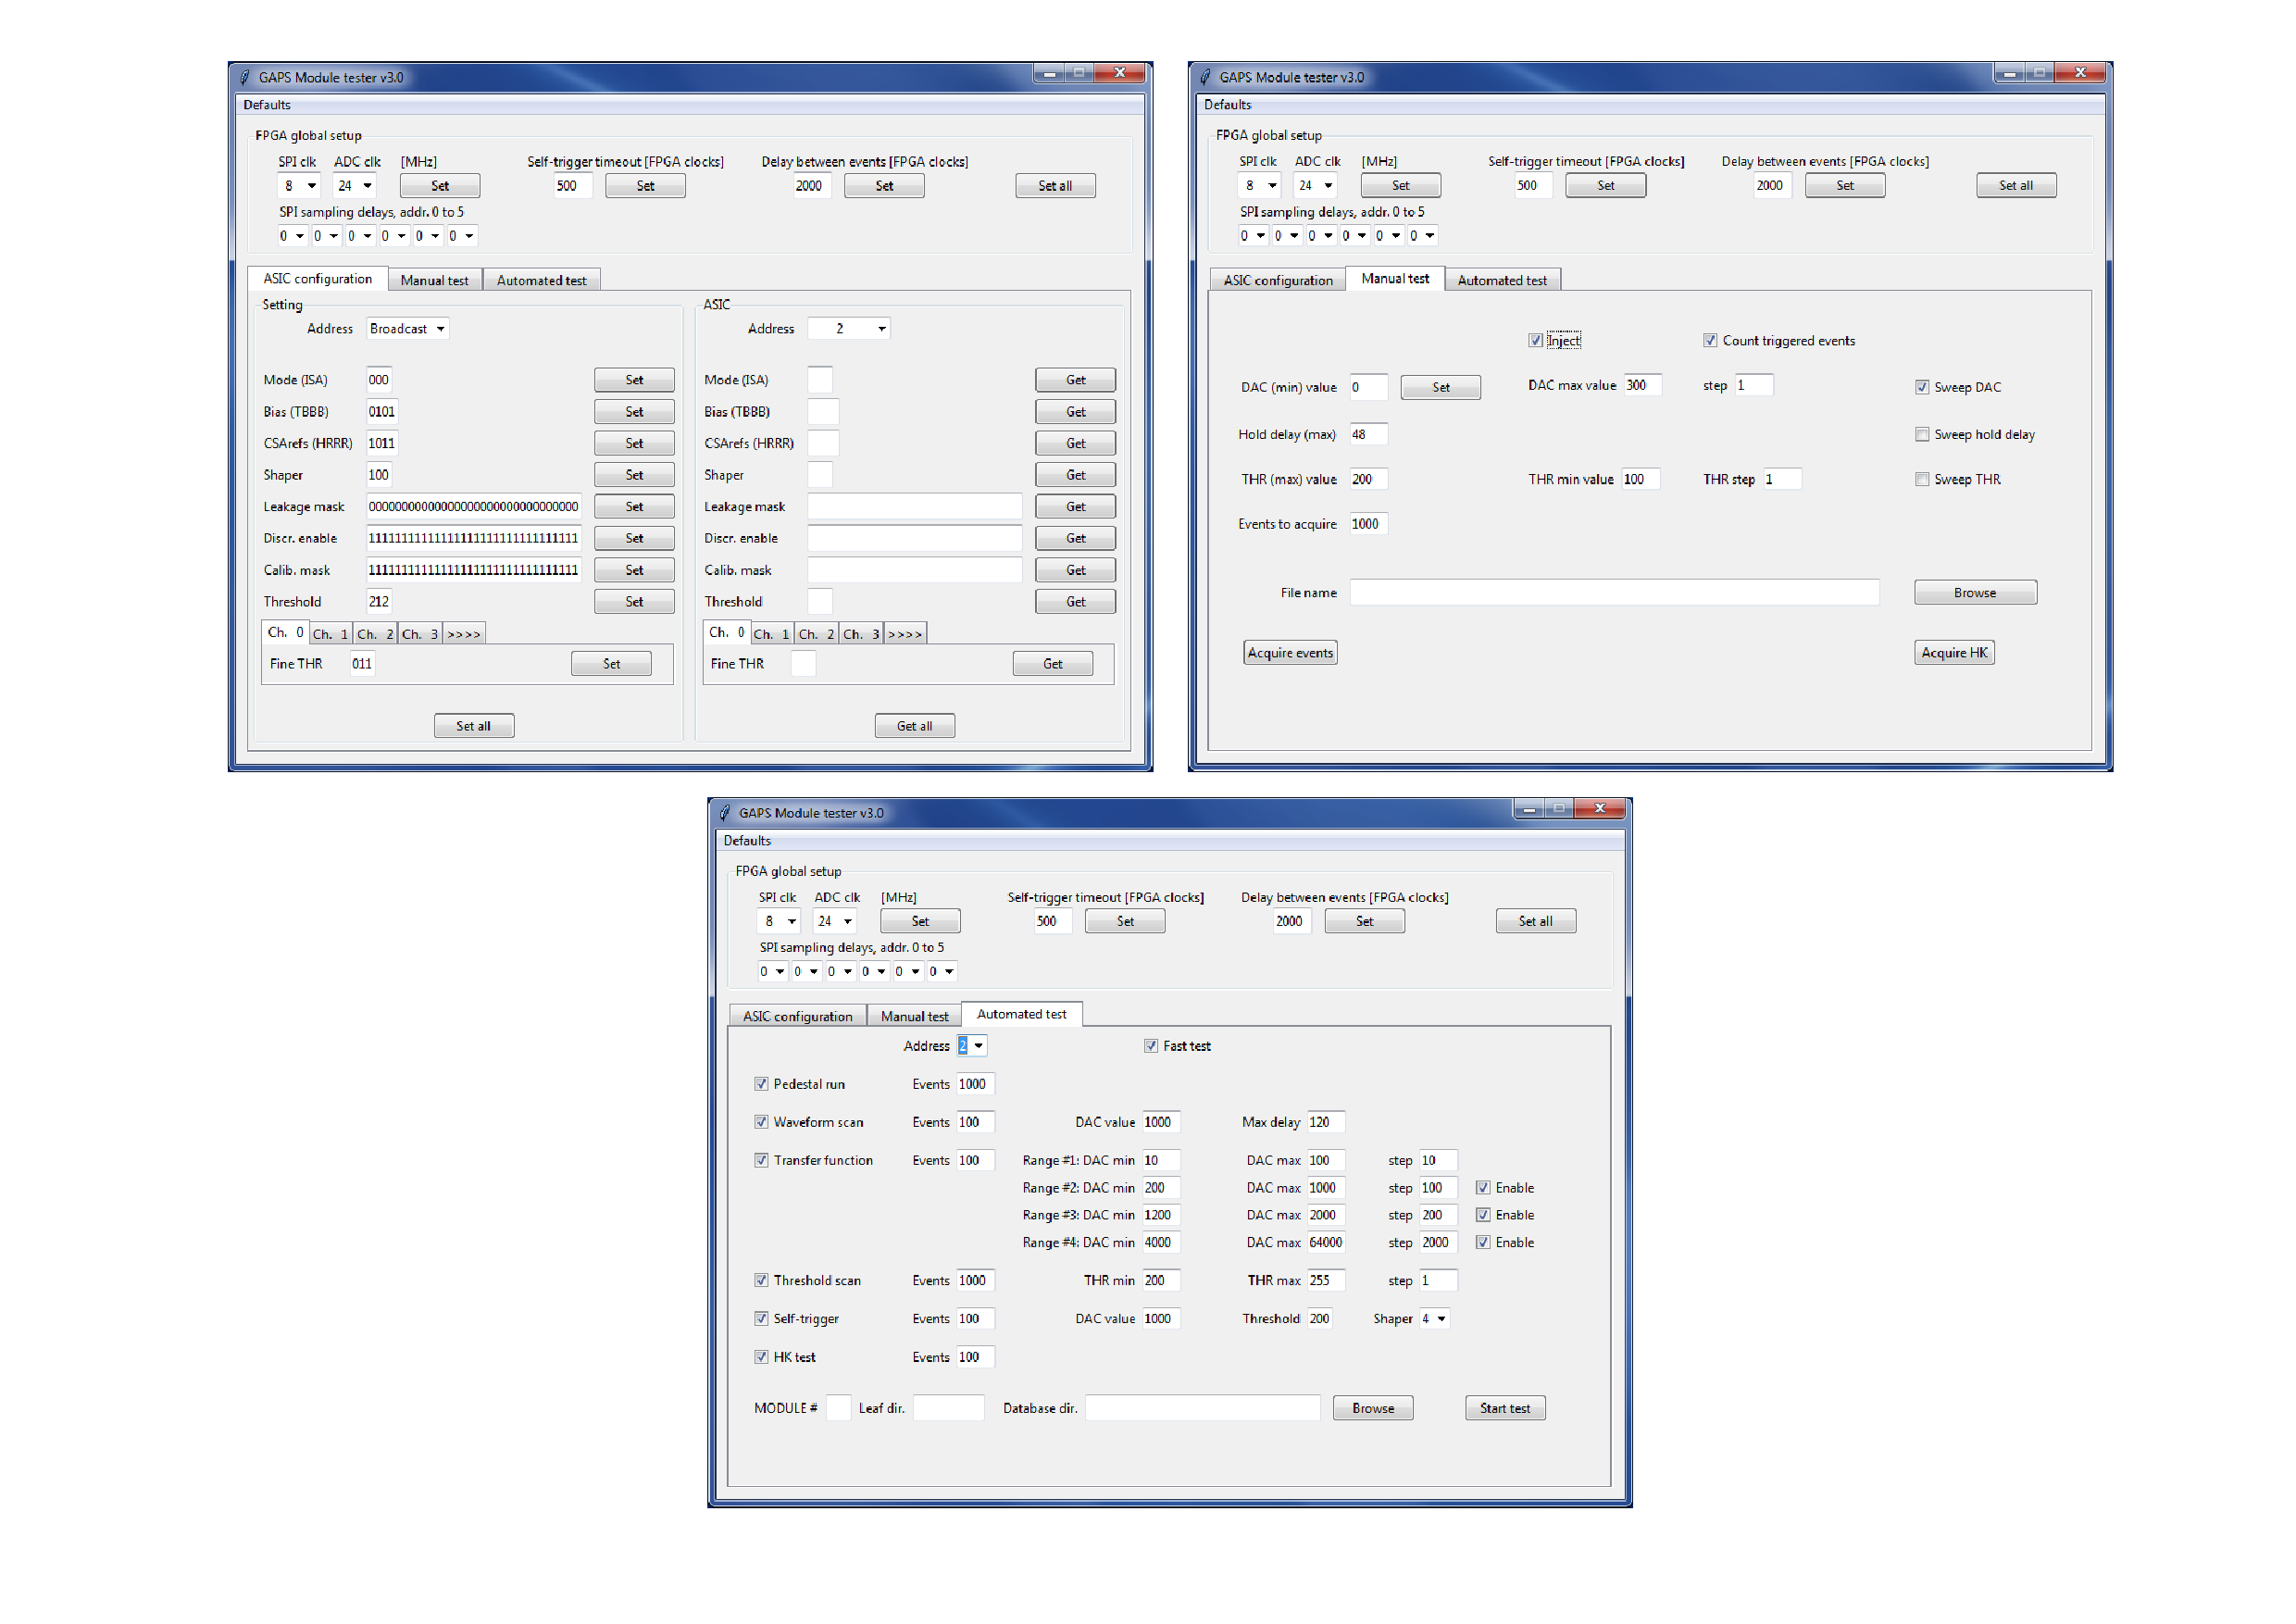
\includegraphics[width=0.97\textwidth]{Images/chap2/moduletester.pdf}
    \caption{\texttt{GAPS\_ModuleTester} main interfaces (clockwise from top-left): ASIC configuration, Manual Test, Automated Test.}
    \label{figmodtest}
\end{figure}

\par
The first interface, called \textit{ASIC configuration}, is dedicated to the configuration of the ASIC, namely its address, registers and configuration bits, specifically:

\begin{enumerate}
    \itemsep0em 
    \item OPERATING MODE (\texttt{ISA} bit);
    \item GLOBAL BIAS REGULATION (\texttt{TBBB} bits); %, where bit \texttt{T} is not used in SLIDER32);
    \item CSA REFERENCE REGULATION (\texttt{HRRR} bits, where bit \texttt{H} is set to \texttt{1} at ambient temperature and \texttt{0} at \SI{-40}{\celsius});
    \item SHAPER TIME CONSTANT (\texttt{TTT} bit);
    \item DISCRIMINATOR ENABLE MASK (32 bit mask for channel activation);
    \item LEAKAGE CURRENT MASK (for leakage current measurements);
    \item CALIBRATION MASK (for calibration purposes).
\end{enumerate}

\noindent
Through this interface it is also possible to set the global threshold (DISCRIMINATOR THRESHOLD, 8 bit) and the fine threshold for each channel (FINE THRESHOLD, 3 bit). A detailed description of the aforementioned configuration bits can be found in \hyperref[tabSPIcommand]{Table \ref{tabSPIcommand}} that presents the SPI commands accepted by the digital section of the ASIC. 

\par
The \textit{Manual test} interface allows to configure all parameters in order to perform a manual test, like the 16-bit DAC values range for injection (expressed in DAC units), the time interval between injections (expressed in FPGA clocks, where one FPGA clock is equivalent to $\approx \SI{20.83}{\nano\second}$, since the FPGA operates at a frequency of \SI{48}{\mega\hertz}) and the number of events to acquire. It is also necessary to set the output folder path which will contain the configuration parameters and the data generated by the test itself.

\begin{table}[h!]
    \centering
    \resizebox{1\columnwidth}{!}{
        \begin{tabular}{l l l l} 
            \Xhline{2\arrayrulewidth}
            Command name & Command code & Input data & Output data \T\B \\
            \hline
            READ EVENT DATA & \texttt{00000xxx} & $\minus$ & Event data packet \T\B \\
            READ SEU FLAGS/TEMPERATURE SENSOR & \texttt{00001xxx} & $\minus$ & SEU \& Temperature word \T\B \\
            READ OPERATING MODE & \texttt{00010xxx} & $\minus$ & \texttt{00000ISA} \T\B \\
            READ SHAPER TIME CONSTANT & \texttt{00011xxx} & $\minus$ & \texttt{00000TTT} \T\B \\
            READ CSA REFERENCE REGULATION & \texttt{00100xxx} & $\minus$ & \texttt{0000HRRR} \T\B \\
            READ GLOBAL BIAS REGULATION & \texttt{00101xxx} & $\minus$ & \texttt{0000TBBB} \T\B \\
            READ LEAKAGE CURRENT MASK & \texttt{00111xxx} & $\minus$ & 32 bit word \T\B \\
            READ DISCRIMINATOR ENABLE MASK & \texttt{01000xxx} & $\minus$ & 32 bit word \T\B \\
            READ CALIBRATION MASK & \texttt{01001xxx} & $\minus$ & 32 bit word \T\B \\
            READ DISCRIMINATOR THRESHOLD & \texttt{01010xxx} & $\minus$ & \texttt{DDDDDDDD} \T\B \\
            READ FINE THRESHOLD ADJ. CH. \texttt{NNNNN} & \texttt{011NNNNN} & $\minus$ & \texttt{00000FFF} \T\B \\
            WRITE OPERATING MODE & \texttt{10010ISA} & $\minus$ & $\minus$ \T\B \\
            WRITE SHAPER TIME CONSTANT & \texttt{10011TTT} & $\minus$ & $\minus$ \T\B \\
            WRITE CSA REFERENCE REGULATION & \texttt{v10100xxx} & \texttt{0000HRRR} & $\minus$ \T\B \\
            WRITE GLOBAL BIAS REGULATION & \texttt{10101xxx} & \texttt{0000TBBB} & $\minus$ \T\B \\
            SET CALIBRATION DAC VOLTAGE & \texttt{10110xxx} & 16 bit word & $\minus$ \T\B \\
            WRITE LEAKAGE CURRENT MASK & \texttt{10111xxx} & 32 bit word & $\minus$ \T\B \\
            WRITE DISCRIMINATOR ENABLE MASK & \texttt{v11000xx}x & 32 bit word & $\minus$ \T\B \\
            WRITE CALIBRATION MASK & \texttt{11001xxx} & 32 bit word & $\minus$ \T\B \\
            WRITE DISCRIMINATOR THRESHOLD & \texttt{11010xxx} & \texttt{DDDDDDDD} & $\minus$ \T\B \\
            WRITE FINE THRESHOLD ADJ. CH. \texttt{NNNNN} & \texttt{111NNNNN} & \texttt{00000FFF} & $\minus$ \T\B \\
            \Xhline{2\arrayrulewidth}
        \end{tabular}
    }
    \caption{SPI commands and configuration bits.}
    \label{tabSPIcommand}
\end{table}

\par
The last section concerns the \textit{Automated test} that has been used in order to perform the validation of the front-end boards. The automated test carried out on each FEB generates a folder containing the raw data acquired from the board, in the form of \texttt{.dat} files, and it has the following structure.\\

\vspace{-0.3cm}
\dirtree{%
.1 MODULE\_000\_fast/.
.2 1/.
.2 data/.
.3 ConfigurationTest.dat.
.3 HK\_Leakage\_chX.dat.
.3 Pedestal\_tauY.dat.
.3 SelfTrigger\_chX.dat.
.3 ThresholdScan\_fthrZ\_tauY.dat.
.3 TransferFunction\_fast\_tauY.dat.
.3 WaveformScan\_fast\_tauY.dat.
} 

\noindent
where \texttt{X} represents the channel identifier number that spans from 0 to 31, while \texttt{Y} represents the peaking time, that goes from 0 to 7. Specifically, the content of each of the files is defined as follows.

\begin{enumerate}
    \itemsep0em 
    \item \texttt{ConfigurationTest.dat}: Basic communication and configuration tests.
    \item \texttt{HK\_Leakage\_chX.dat}: Leakage current measurement (to be done with detectors).
    \item \texttt{Pedestal\_tauY.dat}: Pedestal test, in which the baseline variations due to electronic noise are measured. This test evaluates the electronic noise within the channel, measuring its output without injecting any charge. The output signal is therefore purely attributable to noise.
    \item \texttt{SelfTrigger\_chX.dat}: Self-trigger measurement, which reports the output of the ASIC channel (in ADU) obtained with a fixed DAC injection code and using the automatic peak detection feature of the Zero Crossing circuit, described in \hyperref[zeroCrossing]{Appendix \ref{zeroCrossing}}.
    \item \texttt{ThresholdScan\_fthrZ\_tauY.dat}: Threshold measurement, which reports the number of comparator hits, obtained by varying the global threshold word over its range and injecting 1000 times with a fixed DAC code at each step.
    \item \texttt{TransferFunction\_fast\_tauY.dat}: Transfer function measurement, which lists the channel output ADC code obtained by sweeping the calibration DAC code over its range.
    \item \texttt{WaveformScan\_fast\_tauY.dat}: Waveform scan, which reports the output ADC code sampled at delayed times making possibile to reconstruct the shaper transient response.
\end{enumerate}

\noindent
After the data acquisition process, a MATLAB script is run in order to analyse and plot all the tests results, and the output folder has the following structure.\\

\vspace{-0.3cm}
\dirtree{%
.1 MODULE\_000/.
.2 1/.
.3 analysis\_matlab/.
.4 ENC/.
.4 Pedestal/.
.4 SelfTrigger/.
.4 ThresholdScan/.
.4 TransferFunction/.
.4 WaveformScan/.
} 

\noindent
Each sub-directory contains the following:

\begin{enumerate}
    \itemsep0em 
    \item \texttt{ENC}: Equivalent Noise Charge (ENC) elaborated data and plots obtained from pedestal and transfer function (high gain) processing.
    \item \texttt{Pedestal}: Pedestal elaborated data and plots representing the dispersion of the baseline due to electronic noise.
    \item \texttt{SelfTrigger}: Self trigger plots (histograms) representing dispersion of the value read at the output of the ADC triggered by the Zero Crossing circuit.
    \item \texttt{ThresholdScan}: Threshold scan elaborated data and plots reporting the statistics on the threshold obtained through fitting the data with an error function and a threshold dispersion minimisation analysis.
    \item \texttt{TransferFunction}: Transfer function elaborated data and plots, representing channel input/output characteristic.
    \item \texttt{WaveformScan}: Waveform scan elaborated data and plots representing the shaper transient response.
\end{enumerate}

%-------------------------------------------------------------------------------

\subsection{Visual inspection} \label{FEBdefects}

A manual visual inspection has been performed on each FEB by looking over the board either with the naked eye or through magnification. The board has been compared to the design documents to ensure that all specifications were met. The purpose of this activity was to look for common defaults (missing or bad-soldered components) and defects (pits, dents, scratches, pinholes and other defects on printing traces and pads). If no or negligible defects were found, \texttt{[YES]} has been reported in the \textit{Visual Inspection} field of the test report module, similar to the one shown in \hyperref[figF065I]{Figure \ref{figF065I}}. If a missing or bad-soldered component was found, the board was reworked and the operation has been reported in the \textit{Notes} section of the report. A brief description of the most common visual defects that have been categorised is available in \hyperref[figScratches]{Figure \ref{figScratches}}.

\begin{figure}[ht]
    \centering
    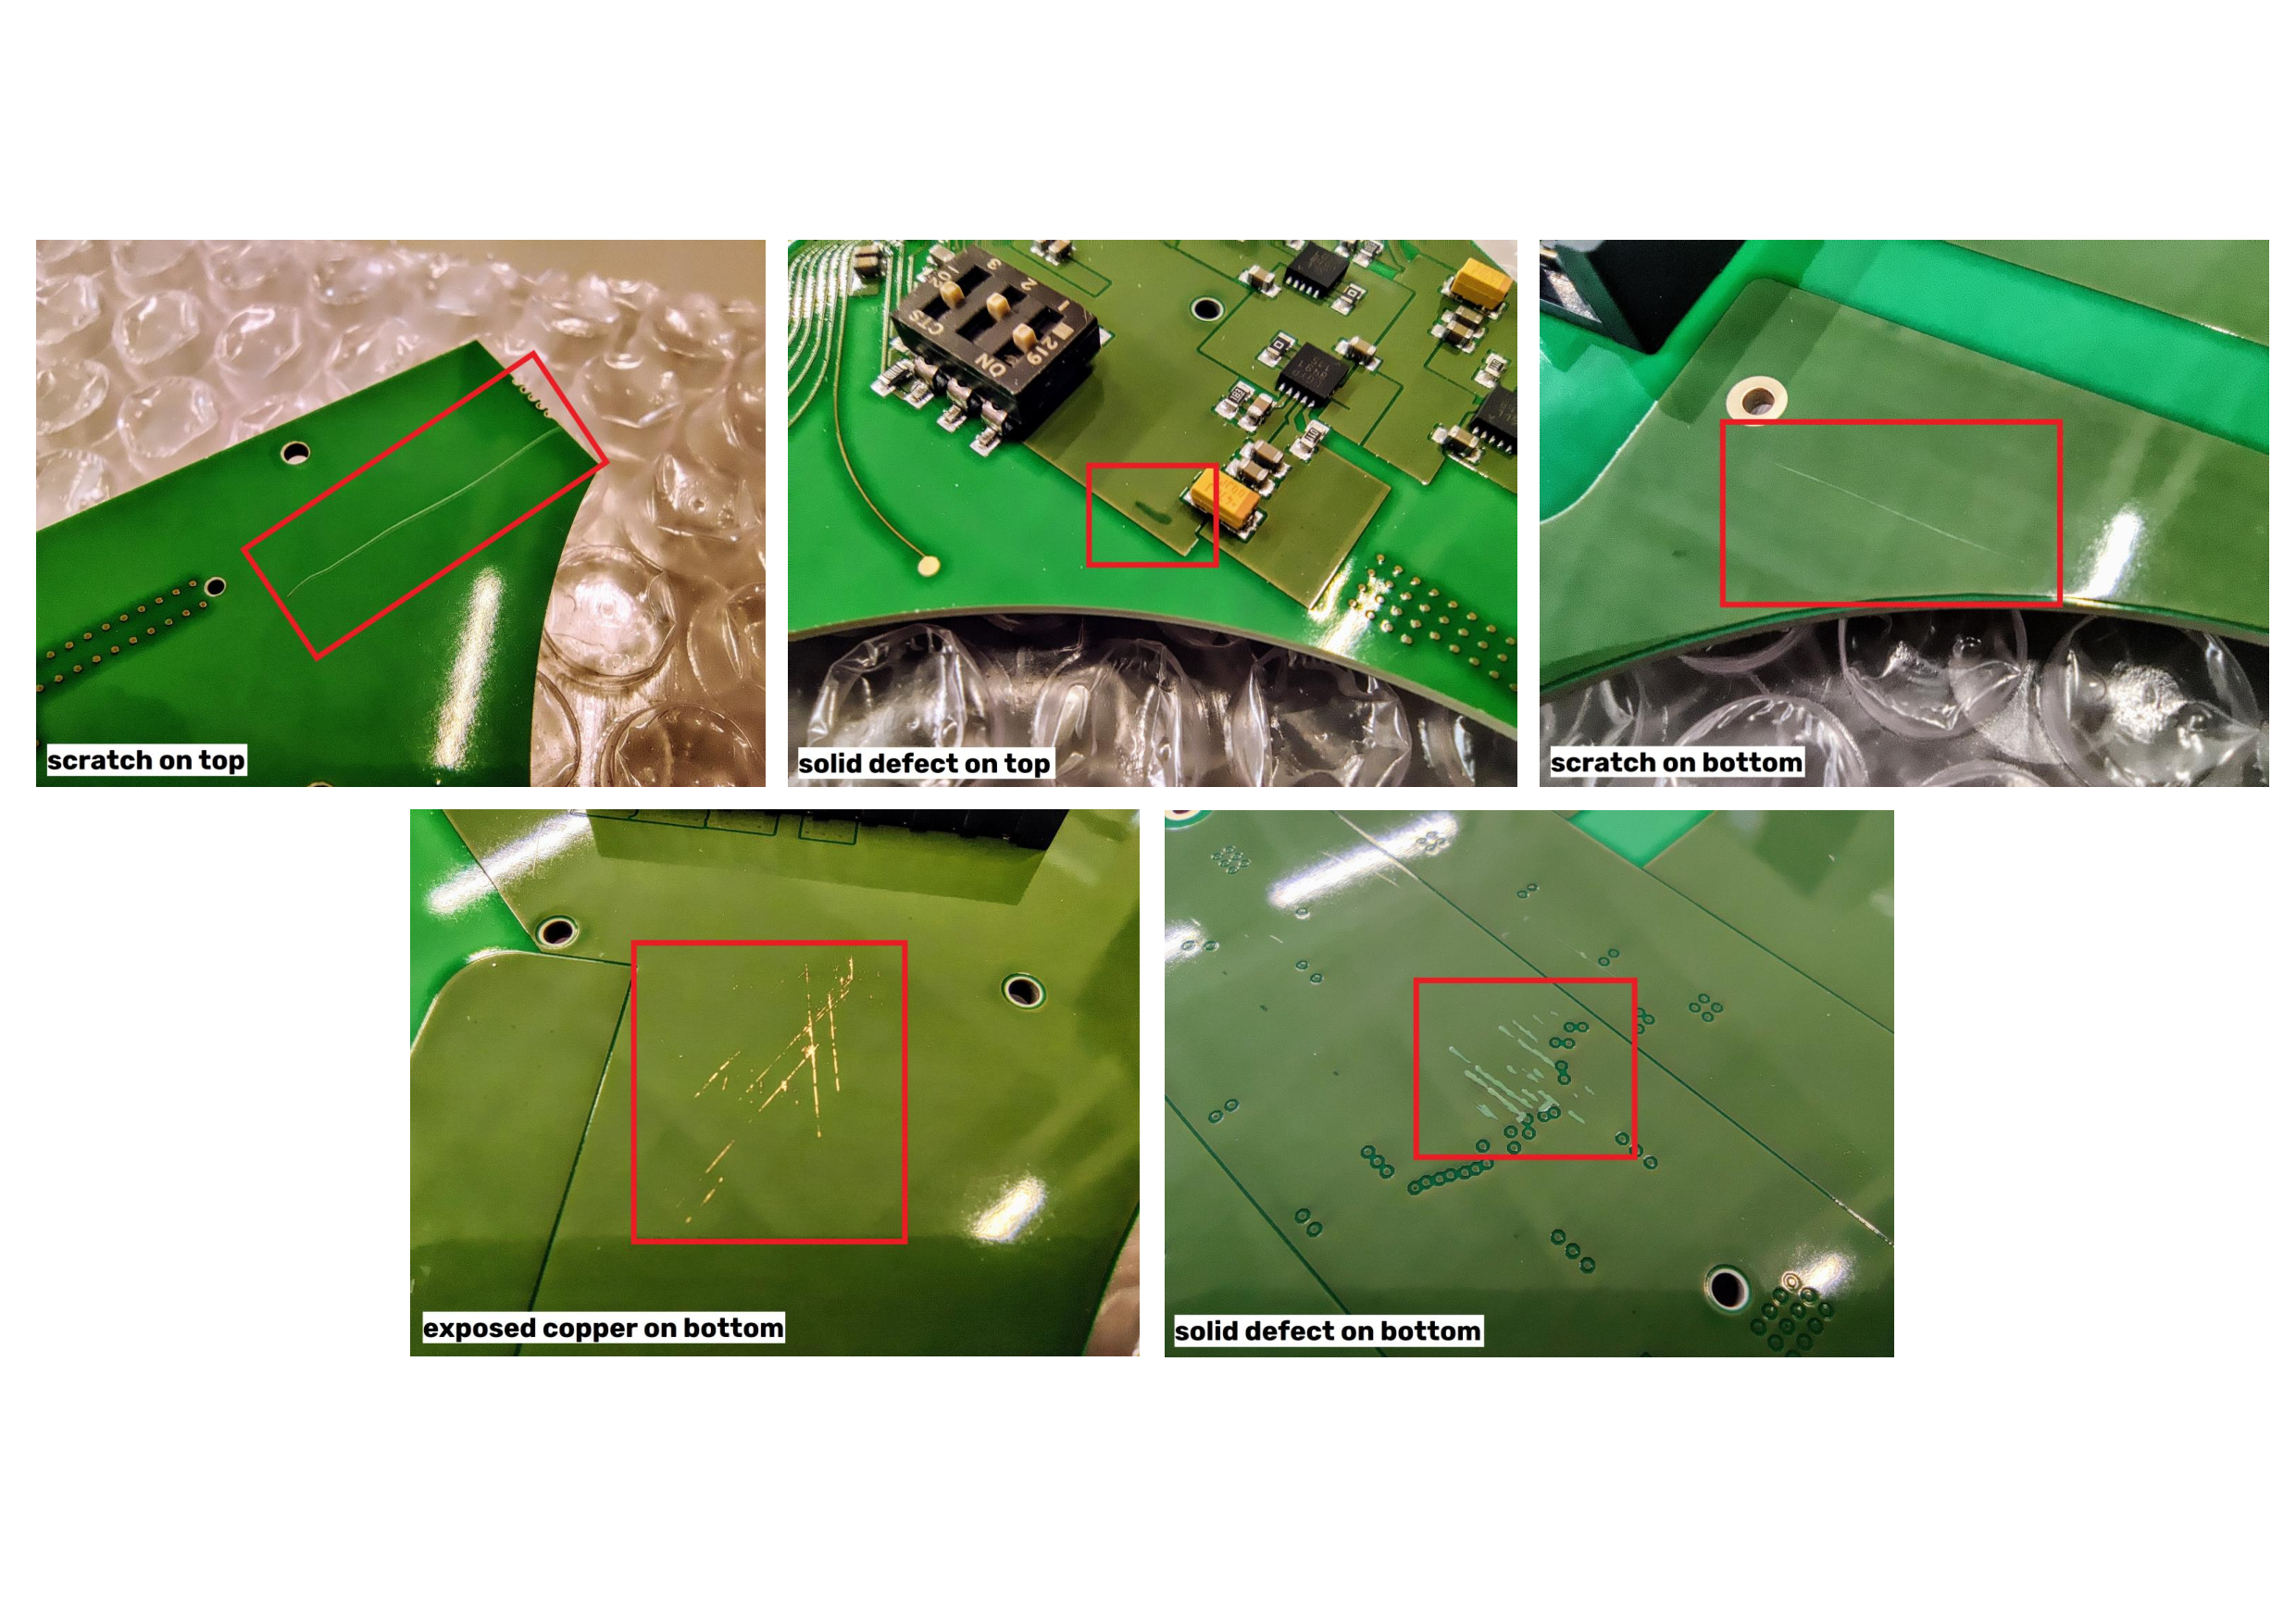
\includegraphics[width=1\textwidth]{Images/chap2/immagini_difetti.pdf}
    \caption{Examples of defects found during visual inspection of the FEBs (clockwise from top-left): scratch on top, solid defect on top, scratch on bottom, exposed copper on bottom, solid defect on bottom.}
    \label{figScratches}
\end{figure}

\par
It is important to emphasise the fact that the visual analysis to search for defects on the board or the components installed on it was of paramount importance in identifying problems that could have altered the proper functioning of the FEB. For example, if there was exposed copper in contact with other metals on the board, short circuits could possibly occur. Furthermore, in the event that a defect in one of the metal layers of the board was very large, this could result in a change in the resistance value of the entire metal layer (e.g. a power supply or a ground), thereby affecting the power consumption and thus altering the nominal operation of the board. In the event that one of the aforementioned defects led to the partial or total non-functioning of the board, the latter was categorised as "reworked" and separated from the others. %A total of 8 FEBs of Italian production and 2 of the US production were classified in this way and are intended to be used for testing purposes only.

%-------------------------------------------------------------------------------

\subsection{Bias} \label{bias}

In this test, the DC voltages are measured with a Fluke 79 III digital multimeter and the DC currents are monitored with the built-in amperometer of the Keysight N6705C
DC Power analyser used as power supply. The only exception is for the Ibias current that is derived from the voltage drop on a \SI{100}{\ohm} Surface Mounted Device (SMD) test resistor (\SI{0.1}{\percent} precision) on the FEB. During the test the ASIC is biased with the following configuration: \texttt{TBBB=0101} and \texttt{HRRR=1011}. The DC voltage and DC current measurements are reported respectively in \hyperref[tabvoltages]{Table \ref{tabvoltages}} and \hyperref[tabcurrents]{Table \ref{tabcurrents}}.

\par
For these measurements, the pass/fail criterion is not obvious, so the typical measurement value has been determined iteratively by analysing the results of the measurements carried out on a larger number of boards, whose test results can be found in \hyperref[FEBresults]{Section \ref{FEBresults}}. If a value in the range of $\pm \SI{10}{\percent}$ with respect to the mean was obtained, \texttt{[YES]}
has been reported in the corresponding section of the report.

\begin{table}[ht]
    \centering
    \begin{tabular}{l l l} 
         \Xhline{2\arrayrulewidth}
         Voltage & Nominal & Description \T\B \\
         \hline
         AVDD & \SI{1.80}{\volt} & \makecell[l]{Voltage at the output of the LDO that regulates the  \T \\ (ASIC) analog power supply \B} \\ 
         DVDD & \SI{1.80}{\volt} & \makecell[l]{Voltage at the output of the LDO that regulates \T the \\ (ASIC) digital power supply \B} \\ 
         3V3 & \SI{3.00}{\volt} & \makecell[l]{Voltage at the output of the LDO that regulates \T the \\ (ASIC) calibration power supply \B} \\ 
         VCMSH & \SI{1.20}{\volt} & Reference voltage for the S\&H \T\B \\ 
         VCM & \SI{0.88}{\volt} & Reference voltage for the shaper \T\B \\ 
         RVCM & \SI{0.90}{\volt} & Reference voltage for the ADC \T\B \\ 
         \Xhline{2\arrayrulewidth}
    \end{tabular}
    \caption{List of voltages measured during the bias test of the FEB.}
    \label{tabvoltages}
\end{table}

\begin{table}[ht]
    \centering
    \begin{tabular}{l l l} 
         \Xhline{2\arrayrulewidth}
         Current & Nominal & Description \T\B \\
         \hline
         IAVDD & \SI{136}{\milli\ampere} & \makecell[l]{Current absorbed by the LDO that regulates the (ASIC) \T \\ analog power supply \B} \\
         IDVDD & \SI{4}{\milli\ampere} & \makecell[l]{Current absorbed by the LDO that regulates the (ASIC) \T \\ digital power supply \B} \\ 
         I3V3 & \SI{3}{\milli\ampere} & \makecell[l]{Current absorbed by the LDO that regulates the (ASIC) \T \\ calibration power supply \B} \\ 
         Ibias & \SI{5}{\milli\ampere} & Bias current for the CSA \T\B \\ 
         \Xhline{2\arrayrulewidth}
    \end{tabular}
    \caption{List of currents measured during the bias test of the FEB.}
    \label{tabcurrents}
\end{table}

%-------------------------------------------------------------------------------

\subsection{Digital}

In this Section of the test report document, results coming from the \textit{Automated test} of the \texttt{GAPS\_ModuleTester} software  are reported considering the following aspects:

\begin{itemize}
    \itemsep0em 
    \item \textbf{Configuration test}: It checks the capability to write and read registers of the digital back-end section of the ASIC of the board under tests. For the FEBs where the improved setup shown in \hyperref[figFEBtest2]{Figure \ref{figFEBtest2}} has been used, this test also accounts for the capability to communicate with the second FEB in the chain.
    \item \textbf{Wrong address test}: It checks the capability of the ASIC to ignore commands when an address, different to the one hardware coded on the board, is selected.
    \item \textbf{Temperature sensor}: It verifies the response of the ADC when the sensor temperature of the FEB is readout.
    
\end{itemize}

%-------------------------------------------------------------------------------

\subsection{Analog}
\label{FEBanalogtest}
The results reported in this Section of the test report document are relevant to the performance of the analog readout channels of the ASIC. Data is obtained from the \textit{Automated test} of the \texttt{GAPS\_ModuleTester} software. The four main reference tests chosen to be included in the report are listed below.

\paragraph{Channel Input-output characteristic} The purpose of this test is to verify that all the channels respond to the input injected signal and provide the expected input-output characteristic with dynamic signal compression. If zero non-responding channels were found, \texttt{[YES]} has been reported in the \textit{Input-output characteristic} field of the test report document.

\paragraph{Noise} The noise performance of 6 channels (No. 0, 7, 15, 16, 23 and 31) is expressed in terms of ENC FWHM in \SI{}{\kilo\electronvolt} and results obtained for peaking time \#6 are reported in this Section. Since the measurement conditions of the FEB are not optimised from a noise point of view, it is not expected that the channels provide the minimum ENC. Therefore, a value lower than \SI{200}{\kilo\electronvolt} is considered good enough to have a \texttt{[YES]} assigned. In the case of 135 US-made FEBs, the ENC measurement was carried out by placing the board inside a metal box in order to shield it from any electromagnetic interference present in the measurement environment. In this way, it was possible to measure ENC values that could provide a more faithful representation of the board actual noise performance. The ENC measurements for 6 of the 32 channels of the ASIC are shown in \hyperref[figFEBNoise]{Figure \ref{figFEBNoise}}.

\paragraph{Threshold dispersion} The threshold dispersion of the 32 channels of the ASIC is reported here, before and after the fine trimming procedure that is adopted to minimise the dispersion of the threshold distribution. This test is conducted in order to determine the width (i.e. the standard deviation) of the distribution of threshold values associated with the 32 channels of the readout electronics. In fact, each channel has a threshold value associated with the minimum energy level at which the comparator is triggered: due to variations in the manufacturing process of the transistors constituting the circuit blocks of the channel (a phenomenon known as \textit{transistor mismatch}), these may in fact have associated threshold values lower or higher than the one specified. The purpose of this test is therefore to check how far the threshold value disperses around the set value. The purpose of this test is also to verify the effectiveness of the 3-bit ADC in each channel used to fine-tune the threshold and thus reduce its dispersion.

\paragraph{Pedestal dispersion} The distribution of the pedestal of the 32 readout channels is reported in this Section.\\

\par
Each FEB has been numbered using an alphanumerical identifier, allowing the board to be uniquely recognised during the assembly of the tracker. The identifier number is composed of three parts, as shown below.

\begin{gather*}
    %\useshortskip
    \Large
    \smallunderbrace{\mathrm{F}}_{\text{\clap{1}}} 
    \smallunderbrace{\mathrm{065}}_{\text{\clap{2}}}
    \smallunderbrace{\mathrm{I}}_{\text{\clap{3}}}
\end{gather*}

\noindent
Specifically, each part of the alphanumerical sequence serves the purpose of:

\begin{enumerate}
    \itemsep0em 
    \item \textbf{F}: It classifies the component ("F" as for "Flight", meaning the FEB has installed a SLIDER32 ASIC in the version intended for use in the in-flight experiment).
    \item \textbf{065}: It uniquely represents the specific board via an increasing numerical value, which matches the numerical identifier of the SLIDER32 ASIC installed on the front-end board.
    \item \textbf{I}: It identifies the country of the manufacturer of the board ("I" for the Italian-made FEBs and "U" for the US-made ones).
\end{enumerate}

\par
For each FEB tested, a test report has been generated in order to sum up all the information regarding the whole testing activity carried out on the front-end board. An example of the aforementioned test report is shown in \hyperref[figF065I]{Figure \ref{figF065I}}. 

\normalsize

%-------------------------------------------------------------------------------

\subsection{GAPS-FEB-Report-Generator}
This Section provides a brief description of the Python software that has been developed in order to automatically generate the test reports for the FEBs, as the one shown in \hyperref[figF065I]{Figure \ref{figF065I}}. The code can be found on GitHub at the following \href{https://github.com/lucaghislo/GAPS-FEB-report-generator}{\underline{link}}.

\subsubsection{Software functionalities} \label{GAPSrepfun}
The software works by taking as input two Comma Separated Values (CSV) files reporting the voltage and current measurements taken on the FEBs and the corresponding defects that have been found during the visual inspection, including optional notes, and producing a report summarising all the data both as a Microsoft Word document and a Portable Document Format (PDF) file, the contents of which are shown in \hyperref[figF065I]{Figure \ref{figF065I}}.\\

\noindent
The Python code is basically organised in two parts:

\begin{enumerate}
    \itemsep0em
    \item \texttt{FEB\_report\_fun.py}: It contains all the functions that are used in order to fill in the Word document and to export the corresponding PDF file. This file also contains the functions used to export log files and CSV tables containing a summary of the values obtained during the testing of each individual FEB.
    \item \texttt{FEB\_report\_out.py}: It contains the function calls to the function blocks defined in the previous file and uses them to build the output document.
\end{enumerate}

%-------------------------------------------------------------------------------

\subsubsection{Software structure}
The software is organised into different sub-folders, each one containing specific input or output files, as described in the following directory tree:\\

\vspace{-0.3cm}
\dirtree{%
.1 GAPS-FEB-report-generator/.
.2 configuration/.
.3 config.conf.
.2 CSV\_tables/.
.3 FEB\_testing - Defects.csv.
.3 FEB\_testing - Multimeter.csv.
.2 modules/.
.3 MODULE\_000/.
.3 ....
.2 output/.
.3 FEB\_report\_log.pdf.
.3 FEB\_report\_log.txt.
.3 script\_values.csv.
.3 temperature\_ADC.csv.
.3 temperature\_C.csv.
.2 report\_PDF/.
.3 F000I.pdf.
.3 ....
.2 report\_template/.
.3 test\_report\_FEB.docx.
.2 report\_word/.
.3 F000I.docx.
.3 ....
.2 script\_files/.
.3 FEB\_report\_fun.py.
.3 FEB\_report\_out.py.
}

\vspace{0.5cm}
\noindent
Moreover, each individual item serves the following function.

\begin{enumerate}
    \itemsep0em
    \item \texttt{config.conf}: Configuration file where the user can specify the nation identifier letter (\texttt{nation\_letter} field) of the producer of the board (\texttt{I} for Italy and \texttt{U} for US production), the document version (\texttt{doc\_version} field), the date, the author name and surname and the nationality of the manufacturer (\texttt{Italian} or \texttt{US}). 
    \item \texttt{FEB\_testing - Defects.csv}: CSV file containing a list of the defects found during the visual inspection of the FEBs, as discussed in \hyperref[FEBdefects]{Section \ref{FEBdefects}}.
    \item \texttt{FEB\_testing - Multimeter.csv}: CSV file containing the voltage and current measurements taken on the FEBs, as described in \hyperref[bias]{Section \ref{bias}}.
    \item \texttt{modules} folder: Containing the folders generated by the purposely developed MATLAB script, described in \hyperref[sec21]{Section \ref{sec21}}.
    \item \texttt{FEB\_report\_log.pdf} and \texttt{FEB\_report\_log.txt}: Log file containing a summary of all the reports fields presented in a single, multi-page document format.
    \item \texttt{script\_values.csv}: CSV file containing a summary of the values obtained during the evaluation of the performance of the analog readout channels of the ASIC generated by the \texttt{GAPS\_ModuleTester} testing software, as mentioned in \hyperref[FEBanalogtest]{Section \ref{FEBanalogtest}}.
    \item \texttt{temperature\_ADC.csv} and \texttt{temperature\_C.csv}: CSV files containing the readings of the temperatures in \SI{}{ADU} and \SI{}{\celsius} respectively.
    \item \texttt{report\_PDF/} folder: Folder containing the PDF version of the reports generated by the software.
    \item \texttt{test\_report\_FEB.docx}: Word template used to produce the final test reports in Word and PDF format.
    \item \texttt{report\_word/} folder: Folder containing the Word version of the reports generated by the software.
    \item \texttt{script\_files} folder: Folder containing the two main Python files used to implement the program, as described in \hyperref[GAPSrepfun]{section \ref{GAPSrepfun}}.
\end{enumerate}

\subsubsection{Software usage}
The program can be launched with Python 3 installed on the PC by double-clicking on the \texttt{FEB\_report\_out.py} Python file and by interacting with the command-line interface shown in \hyperref[figReportTerminal]{Figure \ref{figReportTerminal}}.

\begin{figure}[h!]
    \centering
    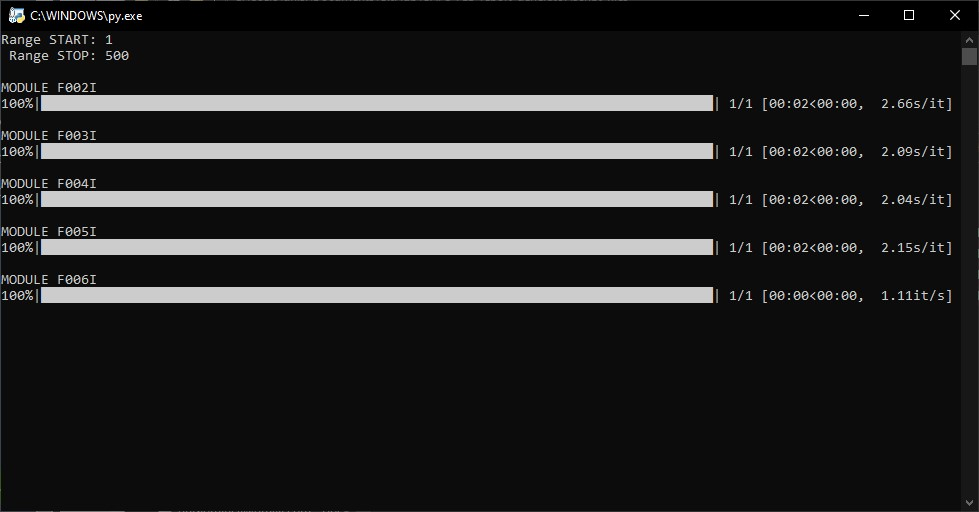
\includegraphics[width=0.8\textwidth]{Images/chap2/rep_gen_terminal.jpg}
    \caption{Command line interface of the \texttt{GAPS-FEB-report-generator} software.}
    \label{figReportTerminal}
\end{figure}

\par
At first, the software asks to input the minimum and maximum values of the FEB identifier numbers for which the user wants to generate a report. It has to be noted that for the program to be correctly executed, \texttt{FEB\_testing - Defects.csv} and \texttt{FEB\_testing - Mutltimeter.csv} have to be present in their corresponding folders. The report generation can be tracked through the loading bars showing the total time taken to compile each report. Once the generation of the reports is complete, the files can be found in \texttt{report\_word/} and \texttt{report\_PDF/} folders respectively.


%-------------------------------------------------------------------------------

\subsection{Analysis of test results} \label{FEBresults}

This Section describes the results of the measurements carried out during the validation phase of the front-end boards. Each graph shows the data distribution for the Italian-made front-end boards (in blue) and US-made ones (in red) separately for comparison purposes. 

\paragraph{AVDD and IAVDD} The graphs in \hyperref[figAVDDIVDD]{Figure \ref{figAVDDIVDD}} show the distributions of the analog supply voltage, AVDD, and the corresponding current IAVDD. The nominal value of AVDD, shown in \hyperref[tabvoltages]{Table \ref{tabvoltages}}, is \SI{1.80}{\volt}, while that of IAVDD, shown in \hyperref[tabcurrents]{Table \ref{tabcurrents}}, corresponds to \SI{136}{\milli\ampere}. It can be seen that both productions present an average voltage value comparable to the nominal one and have the same standard deviation. On the other hand, the average current value is below the nominal one for both productions, with the American one being on average \SI{1.49}{\percent} lower than expected and the Italian one reaching almost exactly the desired current value (\SI{135.93}{\milli\ampere} compared to the \SI{136.00}{\milli\ampere} nominal value).

\begin{figure}[ht]
    \centering
    \begin{tabular}{cc}
        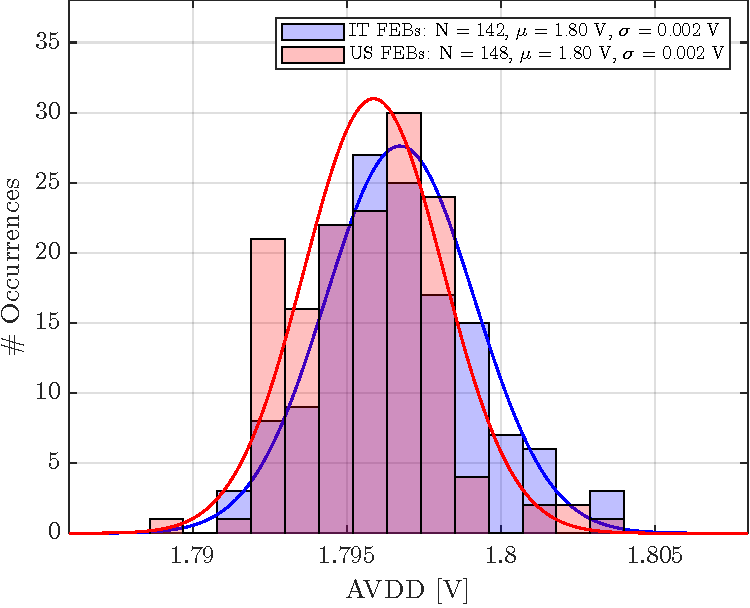
\includegraphics[width=0.475\textwidth]{Images/chap2/results/AVDD.pdf} & 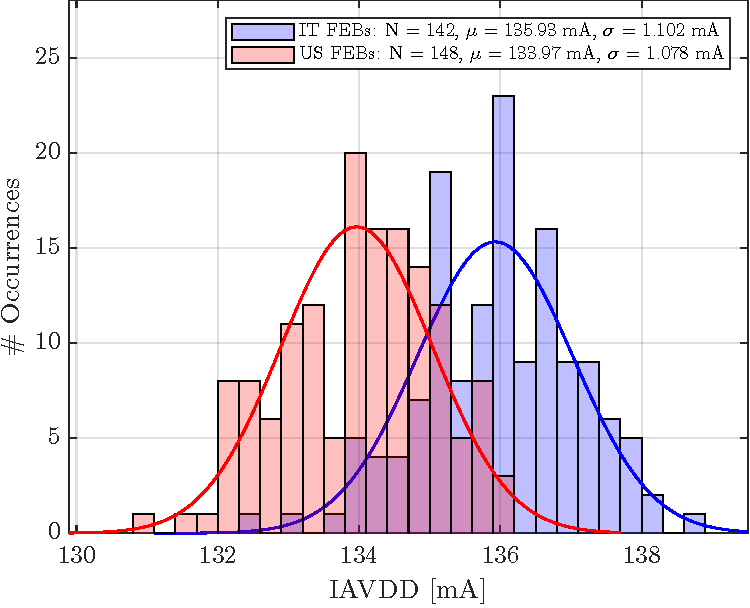
\includegraphics[width=0.475\textwidth]{Images/chap2/results/IAVDD.pdf}\\
    \end{tabular}
    \caption{AVDD values distribution, on the left, and IAVDD values distribution, on the right. Each histogram reports the mean value and standard deviation for both Italian and US productions.}
    \label{figAVDDIVDD}
\end{figure}

\paragraph{Ibias} \hyperref[figFEBIbias]{Figure \ref{figFEBIbias}} shows the distribution of the biasing current, Ibias, whose nominal value is \SI{5}{\milli\ampere}. For both productions, the average value of this parameter is almost comparable with the expected value, with a similar standard deviation between the two.

\begin{figure}[ht]
    \centering
    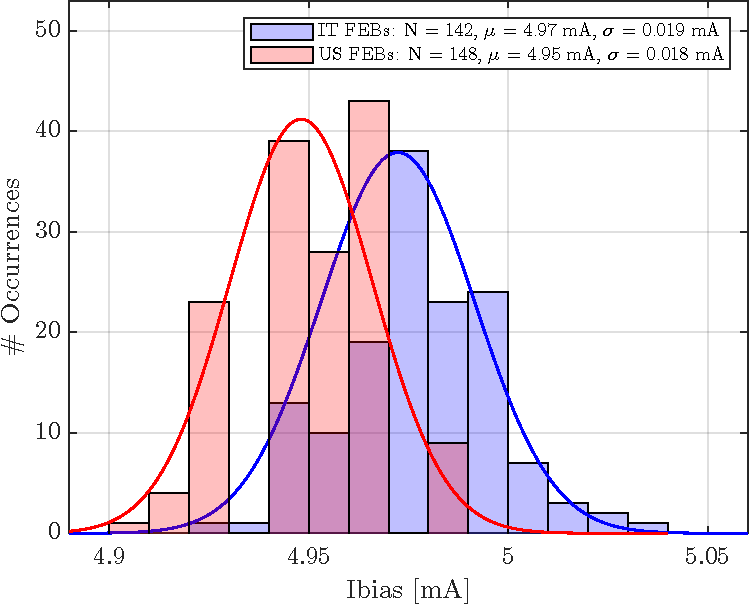
\includegraphics[width=0.475\textwidth]{Images/chap2/results/Ibias.pdf}
    \caption{Ibias values distribution. The histogram reports the mean value and standard deviation for both Italian and US productions.}
    \label{figFEBIbias}
\end{figure}

\paragraph{DVDD and IDVDD} In the case of the digital supply voltage DVDD and the respective current IDVDD, the distributions of the measured values are shown in \hyperref[figDVDDIDVDD]{Figure \ref{figDVDDIDVDD}}. As in the case of the analogue supply voltage, the average values of both outputs are comparable with the nominal value of \SI{1.80}{\volt}. As far as the current is concerned, in the case of the American production, a value of exactly \SI{5.00}{\milli\ampere} was found on all FEBs tested, resulting in a zero standard deviation.

\begin{figure}[h!]
    \centering
    \begin{tabular}{cc}
        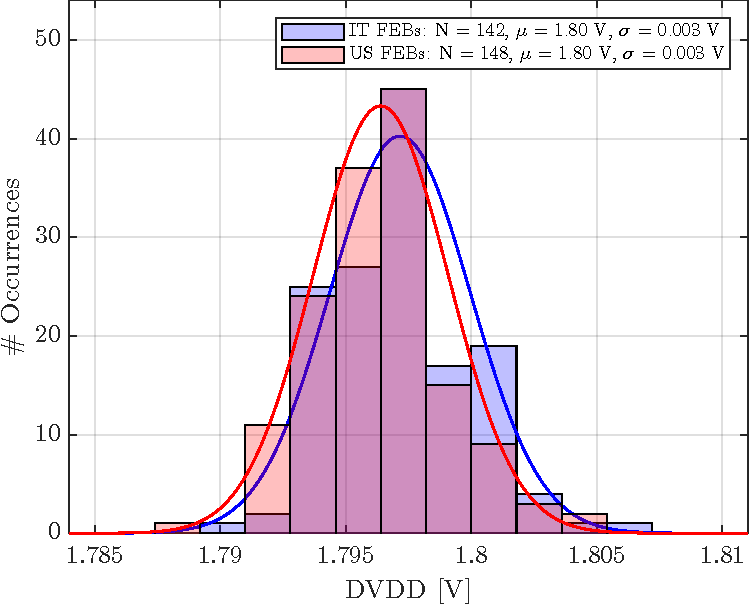
\includegraphics[width=0.467\textwidth]{Images/chap2/results/DVDD.pdf} & 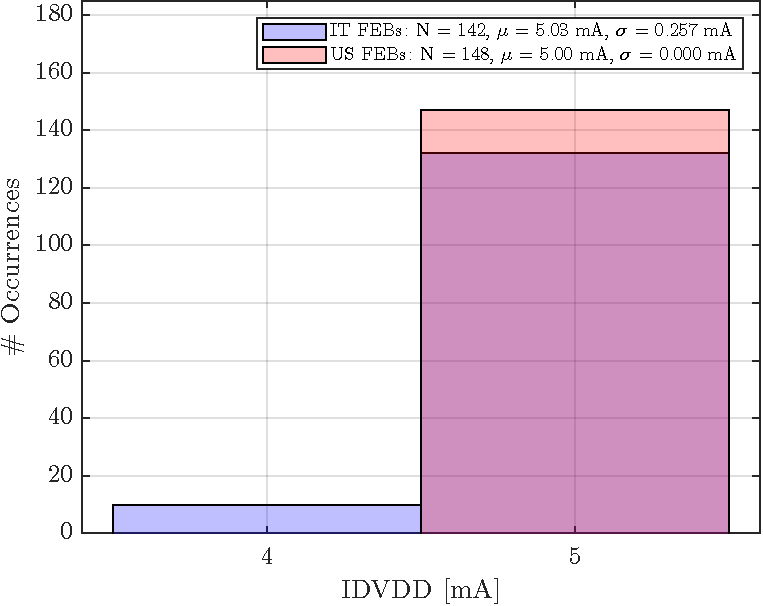
\includegraphics[width=0.477\textwidth]{Images/chap2/results/IDVDD.pdf}\\
    \end{tabular}
    \caption{DVDD values distribution, on the left, and IDVDD values distribution, on the right. Each histogram reports the mean value and standard deviation for both Italian and US productions.}
    \label{figDVDDIDVDD}
\end{figure}

\paragraph{3V3 and I3V3} The distribution of the voltage used as a power supply for calibration, 3V3, and the associated current, I3V3, are shown in \hyperref[fig3V3I3V3]{Figure \ref{fig3V3I3V3}}. It can be seen that the voltage distribution in the case of American production has almost twice the dispersion of Italian production. This phenomenon is attributed to the fact that for 6 FEBs, values greatly different from the expected one are obtained, up to \SI{2.33}{\percent} less. On the other hand, for the Italian production, all measured values are are consistent with the mean, with a standard deviation of \SI{5.00}{\milli\volt}.

\begin{figure}[ht]
    \centering
    \begin{tabular}{cc}
        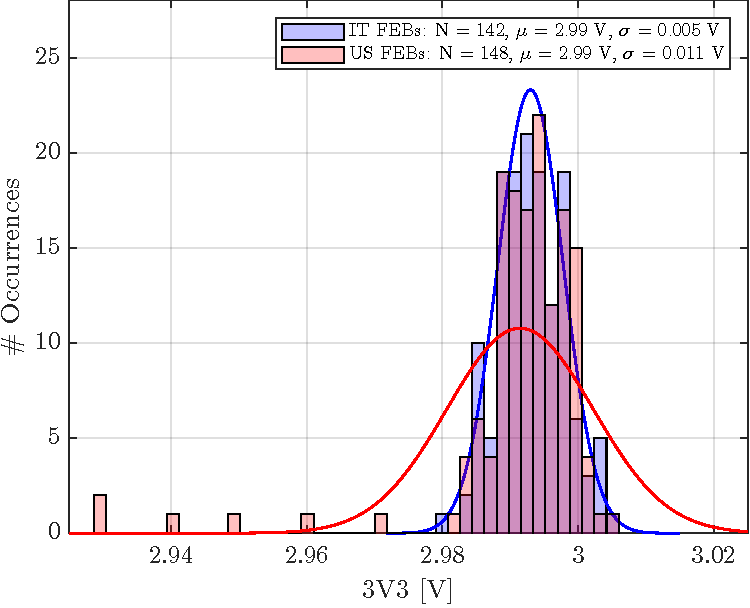
\includegraphics[width=0.467\textwidth]{Images/chap2/results/3V3.pdf} & 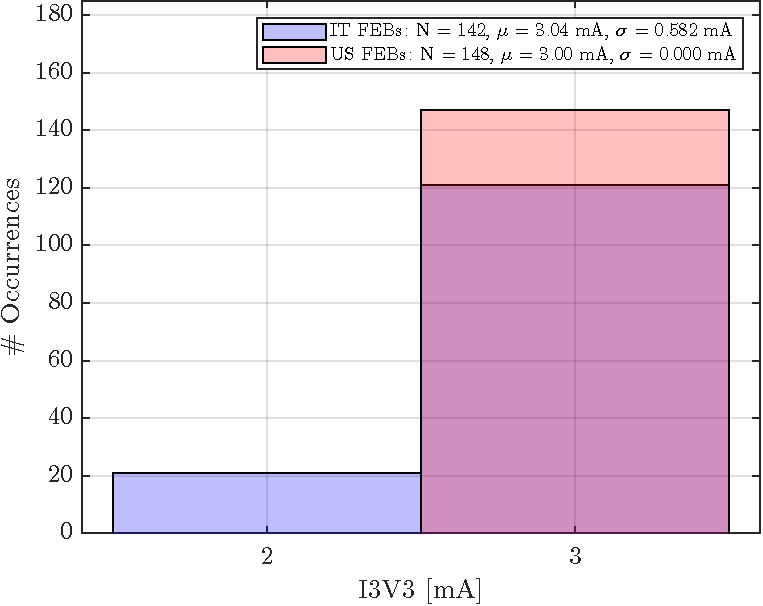
\includegraphics[width=0.477\textwidth]{Images/chap2/results/I3V3.pdf}\\
    \end{tabular}
    \caption{3V3 values distribution on the left and I3V3 values distribution on the right. Each histogram reports the mean value and standard deviation for both Italian and US productions.}
    \label{fig3V3I3V3}
\end{figure}

\begin{figure}[h!]
    \centering
    \begin{tabular}{cc}
        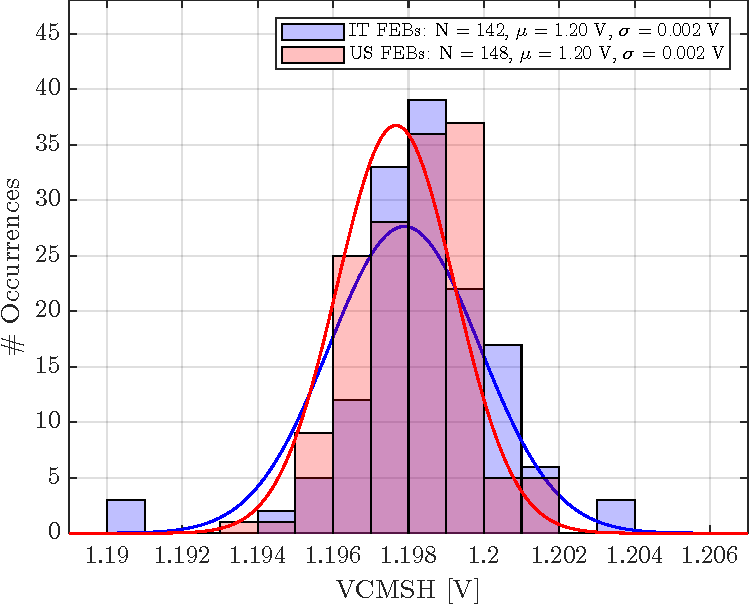
\includegraphics[width=0.475\textwidth]{Images/chap2/results/VCMSH.pdf} & 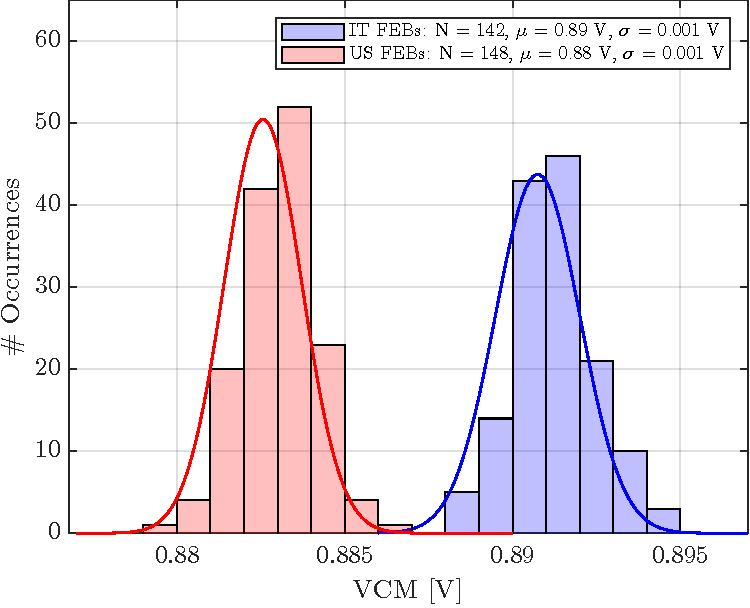
\includegraphics[width=0.475\textwidth]{Images/chap2/results/VCM.pdf}\\
        \multicolumn{2}{c}{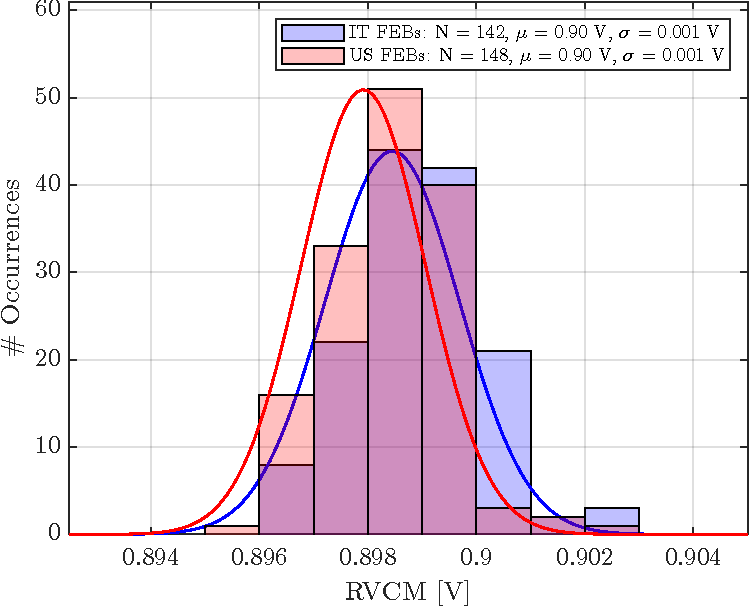
\includegraphics[width=0.475\textwidth]{Images/chap2/results/RVCM.pdf}}
    \end{tabular}
    \caption{Clockwise from left to right: VCMSH, VCM and RVCM values distributions. Each histogram reports the mean value and standard deviation for both Italian and US productions.}
    \label{figVCMSHVCMRVCM}
\end{figure}

\paragraph{VCMSH, VCM and RVCM} \hyperref[figVCMSHVCMRVCM]{Figure \ref{figVCMSHVCMRVCM}} shows the distributions of voltages used as references for the S\&H, shaper and ADC respectively. In the case of VCMSH and RVCM, the average values for both distributions are comparable with the reference value of \SI{1.20}{\volt} and \SI{0.90}{\volt} respectively. In the specific case of the VCM voltage, the Italian and American productions present an average value that differs by approximately \SI{10}{\milli\volt} from each other, while maintaining a comparable standard deviation.

\paragraph{Temperature} The temperature measurements shown in \hyperref[figFEBtemp]{Figure \ref{figFEBtemp}} allows to verify the correct operation of the temperature sensor installed on the front-end board. It can be seen that the average temperature measured on the American-made FEBs is higher than that measured on the Italian-made FEBs. This is purely attributable to the period of the year in which the tests were carried out, that is, summer, therefore an increase in the average measured temperature can be expected. Furthermore, the fact that the tests on the American production were completed within approximately two weeks can be seen in the lower standard deviation, which can be attributed to a smaller fluctuation in ambient temperature. In order to obtain the temperature measurement from the sensor installed on the front-end board (Texas Instruments LMT84), it is first necessary to obtain the output voltage value $V_{T}$, which considering the sensor readout network implemented on the ASIC is evaluated as:

\begin{figure}[h!]
    \centering
    \begin{tabular}{cc}
        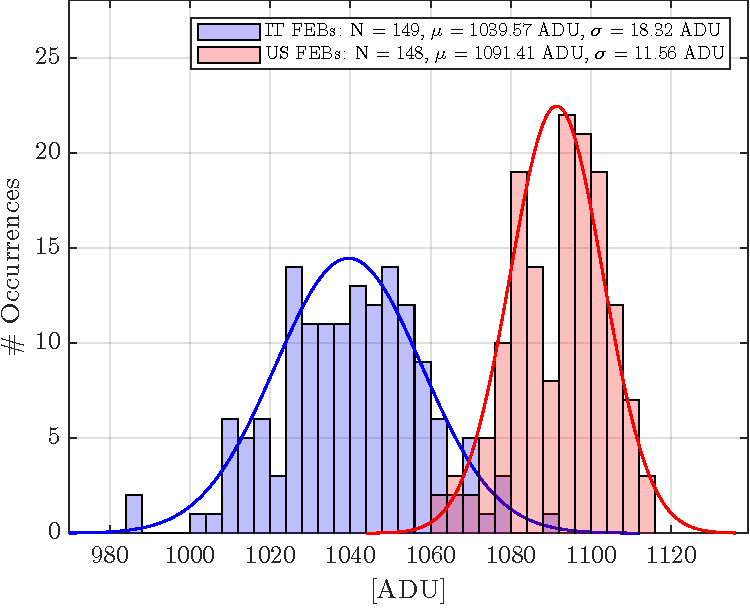
\includegraphics[width=0.475\textwidth]{Images/chap2/results/temperatura_ADC.pdf} & 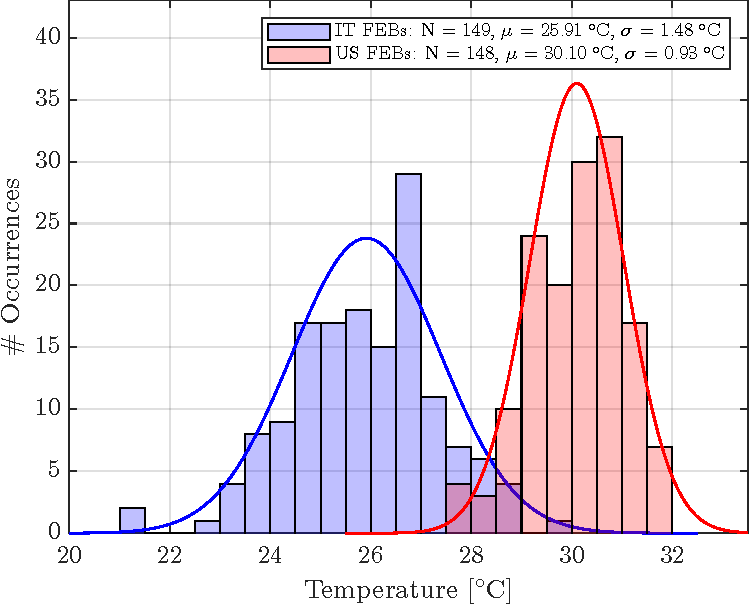
\includegraphics[width=0.475\textwidth]{Images/chap2/results/temperatura_C.pdf}\\
    \end{tabular}
    \caption{Temperature statics for Italian made FEBs: temperature expressed in Analog Digital Units (ADU) on the left and in Celsius (\SI{}{\celsius}) on the right. Each histogram reports the mean value and standard deviation for both Italian and US productions.}
    \label{figFEBtemp}
\end{figure}

% temperature conversion [ADC_code > °C]
% voltage
\begin{equation}
    V_{T} = \SI{900}{\milli\volt} - \frac{(ADC_{code} - 1024) \cdot \SI{1.72}{\milli\volt}}{3.87}.
\end{equation}

\noindent
From this Equation the temperature T can be obtained (expressed in \SI{}{\celsius}):

% temperature
\begin{equation}
    T = \SI{30}{\celsius} + \frac{\SI{5.506}{\frac{\milli\volt}{\celsius}} - \sqrt{(\SI{-5.506}{\frac{\milli\volt}{\celsius}})^2 + 4 \cdot \SI{0.00176}{\frac{\milli\volt}{\celsius^2}} \cdot (\SI{870.6}{\milli\volt} - V_{T})}}{2 \cdot (\SI{-0.00176}{\frac{\milli\volt}{\celsius^2}})}
\end{equation}

\paragraph{Defects detected during visual inspection} \hyperref[figFEBdefects1]{Figure \ref{figFEBdefects1}} shows a comparison of the categories of defects detected on Italian and American-made FEBs during visual inspection, while \hyperref[figFEBdefects2]{Figure \ref{figFEBdefects2}} shows the percentage of FEBs with and without defects detected for both productions. It can be seen that although the percentage of defects detected differs significantly between the two productions, the overall percentage of defect-free front-end boards is comparable.

\begin{figure}[h!]
    \centering
    \begin{tabular}{cc}
        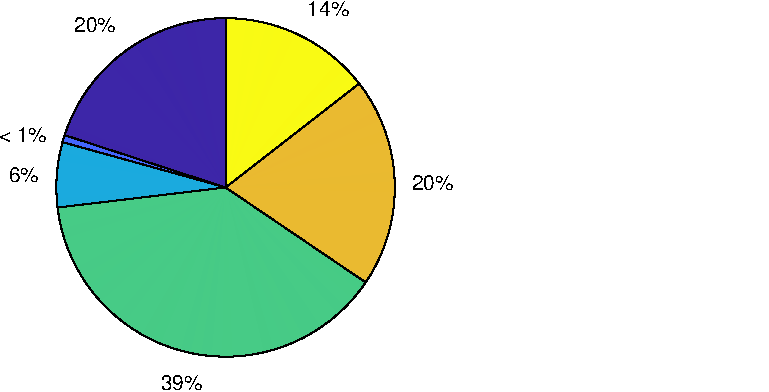
\includegraphics[width=0.35\textwidth]{Images/chap2/results/defects_category_IT.pdf} & 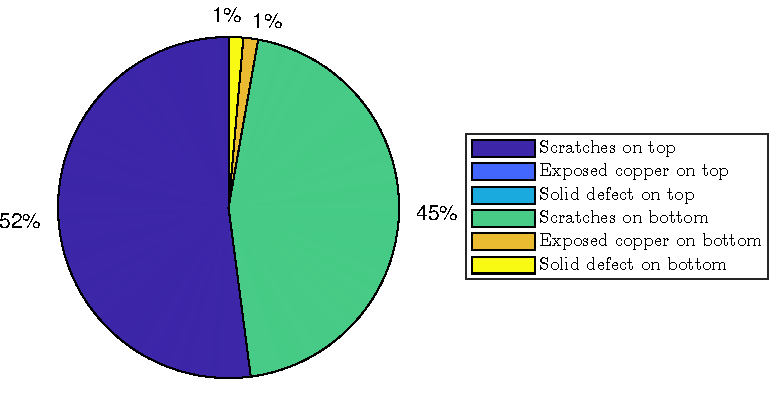
\includegraphics[width=0.58\textwidth]{Images/chap2/results/defects_category_US.pdf}\\
    \end{tabular}
    \caption{Defects found during visual inspection on Italian made FEBs (on the left) and on US-made ones (on the right).}
    \label{figFEBdefects1}
\end{figure}

\begin{figure}[h!]
    \centering
    \begin{tabular}{c p{8.6cm}}
        \includegraphics[width=0.285\textwidth]{Images/chap2/results/defects_number_IT.pdf} & \includegraphics[width=0.6\textwidth]{Images/chap2/results/defects_number_US.pdf}\\
    \end{tabular}
    \caption{Percentage of FEB without any noticeable visual defects for the Italian production (on the left) and for the US production (on the right).}
    \label{figFEBdefects2}
\end{figure}

\paragraph{Pedestal dispersion} This paragraph reports the results of the pedestal measurement used to evaluate the electronic noise of each channel in order to identify the most problematic ones, which could adversely affect the correct measurement of incident charges. The plot in \hyperref[figFEBpedestal]{Figure \ref{figFEBpedestal}} represents the distribution of pedestal dispersion evaluated on the FEBs of Italian and US production. It is easy to deduce how the use of the metal box induces a reduction in pedestal dispersion, which in US-made FEBs is reduced by about \SI{83}{\percent} in mean value and \SI{74}{\percent} in terms of standard deviation compared to Italian-made ones.

\begin{figure}[h!]
    \centering
    \includegraphics[width=0.55\textwidth]{Images/chap2/results/ped_disp.pdf}
    \caption{Pedestal dispersion distribution. The histogram reports the mean value and standard deviation for both Italian and US productions.}
    \label{figFEBpedestal}
\end{figure}

\paragraph{Threshold dispersion} \hyperref[figFEBthreshold]{Figure \ref{figFEBthreshold}} presents the distributions of threshold dispersion before fine threshold optimisation (on the left) and after (on the right). It can be seen that, after optimisation using the 3-bit DAC, both distributions from Italian and US production, have a reduced dispersion as well as a compatible mean and standard deviation since the minimisation process focuses on obtaining a threshold voltage value consistent across all the modules integrated in the tracker. Fine threshold tuning via the aforementioned 3-bit DAC in fact allows the threshold voltage to be optimised directly on the individual channel, thus making it possible to bring the threshold value of the channel closer to the global threshold value. This is made necessary by the fact that, due to variations in the manufacturing process of the transistors constituting the channel circuit blocks, each channel has a threshold value slightly different from one another and not necessarily equal to the set global threshold value. This method therefore allows one to act at a "fine" level in order to reduce the overall threshold dispersion over all 32 channels. 

\par
The result of applying this method is immediately visible by comparing the standard deviations of the distributions shown in \hyperref[figFEBthreshold]{Figure \ref{figFEBthreshold}}, which highlights how the dispersion value after optimisation is on average reduced by half on both productions.

\begin{figure}[h!]
    \centering
    \begin{tabular}{cc}
        \includegraphics[width=0.475\textwidth]{Images/chap2/results/thrdisp_bef.pdf} & \includegraphics[width=0.475\textwidth]{Images/chap2/results/thrdisp_aft.pdf}\\
    \end{tabular}
    \caption{Threshold dispersion values distribution before fine threshold optimisation (on the left) and after (on the right). Each histogram reports the mean value and standard deviation for both Italian and US productions.}
    \label{figFEBthreshold}
\end{figure}

\paragraph{Noise} The noise measurements carried out on 135 of the 150 American-made FEBs are shown in \hyperref[figFEBNoise]{Figure \ref{figFEBNoise}} for channels No. 0, 7, 15, 16, 23, 31. In particular, the displayed measurements were carried out by placing the front-end board under test inside a metal box in order to shield it from the electromagnetic interferences present in the test environment. This made it possible to obtain noise measurements, in the form of ENC, that could effectively reflect the real noise performance of the boards, free of alterations due to the surrounding environment. The remaining FEBs, including those of Italian manufacture, were tested without any shielding and demonstrated ENC values even in the hundreds of \SI{}{\kilo\electronvolt} range.

\begin{figure}[h!]
    \centering
    \begin{tabular}{cc}
        \includegraphics[width=0.475\textwidth]{Images/chap2/results/ENC_0.pdf} & \includegraphics[width=0.475\textwidth]{Images/chap2/results/ENC_7.pdf}\\
        \includegraphics[width=0.475\textwidth]{Images/chap2/results/ENC_15.pdf} & \includegraphics[width=0.475\textwidth]{Images/chap2/results/ENC_16.pdf}\\
        \includegraphics[width=0.475\textwidth]{Images/chap2/results/ENC_23.pdf} & \includegraphics[width=0.475\textwidth]{Images/chap2/results/ENC_31.pdf}\\
    \end{tabular}
    \caption{Statistical distributions of measured ENC FWHM for a limited set of boards belonging to the US production. Each histogram also reports the distribution mean value and standard deviation.}
    \label{figFEBNoise}
\end{figure}


%-------------------------------------------------------------------------------
%   Dummy-1 front-end board
%-------------------------------------------------------------------------------

\section{Dummy-1 front-end board} \label{sec22}

The Dummy board type 1, also known as \textit{Dummy-1}, is a not populated board that will be used in the first launch of the experiment, scheduled for the end of 2023, in order to replace the missing FEBs in some of the detector layers, as these are currently in a smaller number than required to fill all the tracker slots.

The validation tests of the Dummy-1 front-end boards has been performed at ambient temperature after having soldered only a couple of resistors emulating the analog power consumption of the FEB. Specifically, two \SI{40}{\ohm} resistors and a \SI{4.7}{\micro\farad} capacitor 0805 SMD have been installed on the board, along with a short piece of wire ($\approx\SI{1}{\cm}$ in length) in order to connect the newly installed components to the analog voltage supply line, as shown in \hyperref[figDummySoldering]{Figure \ref{figDummySoldering}}. 

\begin{figure}[h!]
    \centering
    \includegraphics[width=0.95\textwidth]{Images/chap2/dummy_image.pdf}
    \caption{Dummy-1 front-end board with a detailed view of the soldered components.}
    \label{figDummySoldering}
\end{figure}

This configuration was chosen as the one better suited to emulate the thermal behaviour of the active components installed on a fully populated FEB. Initial trials were based on a single \SI{20}{\ohm} 0805 SMD resistor directly connected to the AVDD supply voltage, but this configuration was soon discarded as the power dissipated by the resistor was very near to its \SI{0.5}{\watt} maximum power rating. In fact, the current flowing through the resistor is evaluated as

\begin{equation}
    I_{R} = \frac{\SI{2.8}{\volt}}{\SI{20}{\ohm}} = \SI{0.14}{\ampere} = \SI{140}{\milli\ampere} 
\end{equation}

\noindent
therefore the power dissipated by the resistor is

\begin{equation}
    P_{R} = \SI{2.8}{\volt} \cdot \SI{0.14}{\ampere} = \SI{0.392}{\watt} 
\end{equation}

\noindent
which confirms the aforementioned. A common rule of thumb requires the power rating to be at least twice the nominal dissipated power, therefore employing two \SI{40}{\ohm} resistors in parallel allowed the power dissipated on each resistor to be half of the total dissipated power

\begin{equation}
    P_{R} = \SI{2.8}{\volt} \cdot \frac{\SI{0.14}{\ampere}}{2} = \SI{0.196}{\watt}
\end{equation}

\noindent
thus ensuring compliance to the aforementioned rule of thumb. \hyperref[figDummyThermal]{Figure \ref{figDummyThermal}} shows the thermal image for the configuration with a single resistor (on the left) and with two resistors (on the right). In both cases, the analog supply voltage (AVDD) was set to \SI{2.8}{\volt}, as a worst case scenario. It can be seen the temperature difference between the two configurations is of approximately \SI{9.8}{\celsius} for the same dissipated power.

\begin{figure}[h!]
    \centering
    \includegraphics[width=0.8\textwidth]{Images/chap2/DUMMY_bef_aft.pdf}
    \caption{Thermal performance of Dummy-1 boards: on the left the configuration with a single \SI{20}{\ohm} resistor, on the right the configuration with two \SI{40}{\ohm} resistors in parallel.}
    \label{figDummyThermal}
\end{figure}

\par
\noindent
Tests carried out on the Dummy-1 FEBs have the purpose of:

\begin{itemize}
    \itemsep0em 
    \item Verify that the board is able to emulate the proper power dissipation.
    \item Verify that, once placed in series with other FEBs, it is able to properly propagate both bias voltages and digital signals to the subsequent boards.
\end{itemize}

%-------------------------------------------------------------------------------

\subsection{Visual inspection}
A manual visual inspection has been performed for each Dummy-1 sample by looking over the board either with the naked eye or through magnification. Visual inspection has been applied before and after the thermal cycle. The purpose of this activity is to look for missing or bad-soldered ERNI connectors and defects (pits, dents, scratches, pinholes and other defects on printing traces and pads). If no or negligible defects were found, \texttt{[YES]} was reported in the \textit{Visual Inspection} field of the test report module. If a missing or bad-soldered component was found, the board was rejected since it is not possible to manually solder the ERNI connectors.

%-------------------------------------------------------------------------------

\subsection{Thermal test} \label{subsection-thermal}
The boards underwent one thermal cycle in a climate chamber (model ACS DY110) in order to ensure that the board and the components installed on it are not deformed or damaged under the operating temperature conditions of the experiment, thus also verifying the correct soldering of the components on the board. The performed thermal cycle has the following characteristics:

\begin{itemize}
    \itemsep0em 
    \item Minimum temperature (\texttt{$T_{min}$}): \SI{-40}{\celsius}.
    \item Maximum temperature (\texttt{$T_{max}$}): +\SI{60}{\celsius}.
    \item Time spent at $T_{min}$ and $T_{max}$: 20 minutes.
    \item Heating and cooling rate: Maximum \SI{4}{\celsius/minute}.
\end{itemize}

\noindent
If, after the thermal cycle, the PCB did not show any type of defect, \texttt{[YES]} was reported in the \textit{Thermal Cycle} field of the test report module. A plot of the temperature in the climate chamber during thermal test can be found in \hyperref[figDUMMYtest]{Figure \ref{figDUMMYtemp}}, where the \SI{60}{\celsius} and \SI{-40}{\celsius} intervals are visible. It can be also noted that the boards underwent a further 20 minutes at controlled ambient temperature ($\approx\SI{25}{\celsius}$) after the thermal cycle was completed in order to avoid any thermal shocks or damages coming from a sudden change in temperature.

\begin{figure}[h!]
    \centering
    \includegraphics[width=0.6\textwidth]{Images/chap2/chamber_temperature.pdf}
    \caption{Environmental chamber temperature trend during thermal test (in orange) compared to the set-point (in blue).}
    \label{figDUMMYtemp}
\end{figure}

After the thermal cycle, the boards have been left biased for at least 10 minutes. If no damage occurred to the resistors, the test is considered as passed. Moreover, a thermal picture of the resistor has been taken (with a FLIR ETS320 non-contact thermal measurement system), like the one shown in \hyperref[figDummyThermal]{Figure \ref{figDummyThermal}}.

%-------------------------------------------------------------------------------

\subsection{Power test}
In this test a nominal voltage of \SI{2.8}{\volt} was applied to the board. The current IAVDD absorbed and the voltage APDD of the dummy resistor have been measured and reported on the test report together with the computed power consumption PAVDD. For these measurements, the pass/fail criterion is not obvious, so the typical measurement value has been determined iteratively by analysing the scans of a larger number of boards.

%-------------------------------------------------------------------------------

\subsection{Bias and Digital}
The purpose of this test is to validate the soldering of the input and output ERNI connectors. The board under test has been placed in series with a fully populated FEB as shown in \hyperref[figFEBtest2]{Figure \ref{figFEBtest2}} and a configuration test was run on the FEB. If it responded correctly, it means that ERNI connectors on the Dummy-1 board are properly soldered and \texttt{[YES]} has been reported in the \textit{Communication test} field of the test report.

\par
As done for the front-end boards, a test report is generated, whose first page is shown in \hyperref[figDUMMYreport]{Figure \ref{figDUMMYreport}}. In the case of the Dummy-1 front-end boards, a single multi-page document has been created, having the structure described in \hyperref[tabDUMMYstruct]{Table \ref{tabDUMMYstruct}}.

\begin{table}[h!]
    \centering
    \def\arraystretch{1.3}
    \resizebox{0.95\columnwidth}{!}{
        \begin{tabular}{|c|c|c|c|c|c|c|} 
            \hline
            $\bm{\#}$ & \textbf{Board ID} & \makecell{\textbf{Thermal}\T \\ \textbf{cycling}\B} & \makecell{\textbf{Visual}\T \\ \textbf{inspection}\B} & \makecell{\textbf{Communication}\T \\ \textbf{test}\B} & \textbf{IAVDD [\SI{}{\milli\ampere}}]\T\B & \textbf{PAVDD [\SI{}{\milli\watt}}]\T\B \\ 
            \hline
            \texttt{1} & \texttt{D00} & \textcolor{ForestGreen}{\texttt{Yes}}/\textcolor{red}{\texttt{No}} & \textcolor{ForestGreen}{\texttt{Yes}}/\textcolor{red}{\texttt{No}} & \textcolor{ForestGreen}{\texttt{Yes}}/\textcolor{red}{\texttt{No}} & \texttt{000.0} & \texttt{000.00}\T\B \\ \hline 
        \end{tabular}
    }
    \caption{Structure of the entry for the Dummy-1 front-end boards test report.}
    \label{tabDUMMYstruct}
\end{table}

%-------------------------------------------------------------------------------

\subsection{Test results}
This Section reports the results of current (IAVDD) and power (PAVDD) measurements taken on all the 62 Dummy-1 front-end boards. The power value was obtained by multiplying the current value by the resistance value obtained from the parallel of the two installed resistors ($R_{tot} = \SI{20}{\ohm}$). \hyperref[figDUMMYresults]{Figure \ref{figDUMMYresults}} shows the distributions of current values on the left and power values on the right.

\begin{figure}[h!]
    \centering
    \begin{tabular}{cc}
        \includegraphics[width=0.475\textwidth]{Images/chap2/results/dummy/AIDD.pdf} & \includegraphics[width=0.475\textwidth]{Images/chap2/results/dummy/APDD.pdf}\\
    \end{tabular}
    \caption{IAVDD values distribution on the left and PAVDD values distribution on the right. Both plots also provide the mean value and standard deviation of the respective distributions.}
    \label{figDUMMYresults}
\end{figure}


%-------------------------------------------------------------------------------
%   Flex-Rigid Board
%-------------------------------------------------------------------------------

\section{Flex-Rigid Board} \label{flexrigids}

Flex-rigid boards are intended to connect one front-end board with the next in the chain. They are by design flexible and allow digital signals and low power voltage supplies to be transported from one module to the next. The flexibility is given both by the material they are made of, polyamide, and by the presence of ground networks instead of rigid ground planes. The dielectric used in these boards is FR4 and they consist of 7 layers for the rigid zone, at the extremes, where the connectors are located, and 3 for the flexible interconnection zone. \hyperref[figDflexrigidPIC]{Figure \ref{figDflexrigidPIC}} presents on the left a picture of a flex-rigid board next to a photograph in which the flex-rigid board is used to connect two front-end boards, where the flexibility of the flex-rigid board can be appreciated.

\subsection{Visual inspection}
A manual visual inspection has been performed for each sample by looking over the board either with the naked eye or through magnification. Visual inspection is applied before and after the thermal cycle. The purpose of this activity was to look for missing or bad-soldered ERNI connectors and defects (pits, dents, scratches, pinholes and other defects on printing traces and pads). If no or negligible defects were found, \texttt{[YES]} has been reported in the \textit{Visual Inspection} field of the test report. If a missing or bad-soldered component was found, the board is rejected since it is not possible to manually solder the ERNI connectors.

\subsection{Thermal cycle}
The flex-rigid boards underwent one thermal cycle in a climate chamber (model ACS DY110). Thermal cycle has the same characteristics described in \hyperref[subsection-thermal]{section \ref{subsection-thermal}}. For flex-rigid boards that underwent thermal cycle and did not show any type of defect, \texttt{[YES]} has been reported in the \textit{Thermal Cycle} field of the test report.

\subsection{Communication test}
The purpose of this test is to validate the soldering of the two ERNI connectors. The board under test was placed in series with two fully populated FEBs as shown in \hyperref[figFEBtest2]{Figure \ref{figFEBtest2}} and a configuration test was run on the second board in the chain. If it responded correctly, it means that ERNI connectors on the Flex-rigid board are properly soldered and \texttt{[YES]} has been reported in the \textit{Communication test} field of the test report. \\

\begin{figure}[h!]
    \centering
    \begin{tabular}{cc}
        \includegraphics[width=0.38\textwidth]{Images/chap2/flex_rigid_pic.pdf} & \includegraphics[width=0.475\textwidth]{Images/chap2/flex_rigid_two_FEBs.pdf}\\
    \end{tabular}
    \caption{Flex-rigid board (on the left) connected to two front-end board in series, where its flexibility can be appreciated.}
    \label{figDflexrigidPIC}
\end{figure}

\par
As done for the front-end boards, a test report has been generated, whose first page is shown in \hyperref[figFLEXreport]{Figure \ref{figFLEXreport}}. In the case of the flex-rigid boards, a single multi-page document has been produced, having the following structure:

\begin{table}[h!]
    \centering
    \def\arraystretch{2}
    \resizebox{0.6\columnwidth}{!}{
        \begin{tabular}{|c|c|c|c|c|} 
            \hline
            $\bm{\#}$ & \textbf{Board ID} & \makecell{\textbf{Thermal}\T \\ \textbf{cycling}\B} & \makecell{\textbf{Visual}\T \\ \textbf{inspection}\B} & \makecell{\textbf{Communication}\T \\ \textbf{test}\B} \\ 
            \hline
            \texttt{1} & \texttt{FR000} & \textcolor{ForestGreen}{\texttt{Yes}}/\textcolor{red}{\texttt{No}} & \textcolor{ForestGreen}{\texttt{Yes}}/\textcolor{red}{\texttt{No}} & \textcolor{ForestGreen}{\texttt{Yes}}/\textcolor{red}{\texttt{No}}\T\B \\ \hline 
        \end{tabular}
    }
    \caption{Structure of the entry for the flex-rigid boards test report.}
    \label{tabFLEXstruct}
\end{table}


%-------------------------------------------------------------------------------
%   Connector for termination
%-------------------------------------------------------------------------------

\section{Connector for termination}

The purpose of the termination connectors is to adapt the \SI{100}{\ohm} differential digital signal tracks through the use of 10 resistors of \SI{100}{\ohm} each soldered onto the connector. The purpose of the tests performed on the termination connectors was to verify the correct installation of the resistors, as well as to ascertain their correct resistance value.

\begin{figure}[ht]
    \centering
    \includegraphics[width=0.45\textwidth]{Images/chap2/term_conn.pdf}
    \caption{Connector for termination with ten \SI{100}{\ohm} resistors installed.}
    \label{figTermConnector}
\end{figure}

\subsection{Visual inspection}
Visual inspection has been carried out to check the connector quality, then look for misaligned pins or missing termination resistor. Visual inspection is carried out before and after the thermal cycle. If no or negligible defects are found, \texttt{[YES]} is reported in the \textit{Visual Inspection} field of the test report.

\subsection{Thermal cycle}
The connectors underwent one thermal cycle in a climate chamber (model ACS DY110). Thermal cycle has the same characteristics described in \hyperref[subsection-thermal]{section \ref{subsection-thermal}}. For connectors that underwent the thermal cycle, \texttt{[YES]} has been reported in the \texttt{Thermal Cycle} field of the test report.

\subsection{Termination resistor soldering}
The quality of the termination resistor soldering has been verified with a digital multimeter by measuring the resistance seen between two pins on the side of the connector opposite with respect to the one where components are mounted. The test has been performed after the thermal cycle for all the 10 termination resistors. If a value of $\approx100\pm\SI{1}{\ohm}$ is found for all the resistors, \texttt{[YES]} is reported in the \textit{Resistor Soldering} field of the test report module.

\par
As done for the front-end boards, a test report has been generated, whose first page is shown in \hyperref[figTERMCONNreport]{Figure \ref{figTERMCONNreport}}. In the case of the connectors for termination, a single multi-page document has been created:

\begin{table}[ht]
    \centering
    \def\arraystretch{1.3}
    \resizebox{0.65\columnwidth}{!}{
        \begin{tabular}{|c|c|c|c|c|} 
            \hline
            $\bm{\#}$ & \textbf{Connector ID} & \makecell{\textbf{Thermal}\T \\ \textbf{cycling}\B} & \makecell{\textbf{Visual}\T \\ \textbf{inspection}\B} & \makecell{\textbf{Resistor}\T \\ \textbf{soldering}\B} \\ 
            \hline
            \texttt{1} & \texttt{T00} & \textcolor{ForestGreen}{\texttt{Yes}}/\textcolor{red}{\texttt{No}} & \textcolor{ForestGreen}{\texttt{Yes}}/\textcolor{red}{\texttt{No}} & \textcolor{ForestGreen}{\texttt{Yes}}/\textcolor{red}{\texttt{No}}\T\B \\ \hline 
        \end{tabular}
    }
    \caption{Structure of the entry for the termination connectors test report.}
    \label{tabTERMCONNstruct}
\end{table}


%-------------------------------------------------------------------------------
%   Front-end board shields
%-------------------------------------------------------------------------------

\section{Front-end board shields} \label{secShield}

The purpose of the front-end board shields, shown in \hyperref[figShieldsAB]{Figure \ref{figShieldsAB}}, is to cover the tracks connecting the Si(Li) sensor strips with the pins of the readout integrated circuit, thereby reducing the impact of electromagnetic induced noise on each of the 32 channels of the readout ASIC.

\subsection{Visual inspection}
Visual inspection has been carried out to check the surface quality, then look for the existence of pits, dents, scratches, pinholes and other defects. Visual inspection was performed before and after the thermal cycle. If no or negligible defects were found, \texttt{[YES]} has been reported in the \textit{Visual Inspection} field of the test report.

\subsection{Thermal cycle}
The boards underwent one thermal cycle in a climate chamber (model ACS DY110). Thermal cycle has the same characteristics described in \hyperref[subsection-thermal]{section \ref{subsection-thermal}}. For the front-end board shields that underwent the thermal cycle, \texttt{[YES]} has been reported in the \textit{Thermal Cycle} field of the test report.

\begin{comment}
    \begin{figure}[h!]
        \centering
        \begin{tabular}{cc}
            \includegraphics[width=0.5\textwidth]{Images/chap2/shieldsPDFtwo.pdf} & \includegraphics[width=0.3\textwidth]{Images/chap2/Mengjiao_IT_status_PIC.jpg}\\
        \end{tabular}
        \caption{Type A front-end board shield (on the left) and type B front-end board shield (on the right).}
        \label{figShieldsAB}
    \end{figure}
\end{comment}

\begin{figure}[h!]
    \centering
    \includegraphics[width=0.6\textwidth]{Images/chap2/shieldsPDFtwo.pdf}
    \caption{Type A front-end board shield (on the left) and type B front-end board shield (on the right).}
    \label{figShieldsAB}
\end{figure}
    

\begin{comment}
    \begin{figure}[h!]
        \centering
        \includegraphics[width=0.5\textwidth]{Images/chap2/FEB_with_shieldsNO.pdf}
        \caption{Type A and type B front-end board shields mounted on a front-end board.}
        \label{figShieldsMounted}
    \end{figure}
\end{comment}

\par
As done for the front-end boards, a test report has been generated, whose first page is shown in \hyperref[figSHIELDreport]{Figure \ref{figSHIELDreport}}. In the case of the front-end board shields, a single multi-page document has been produced, having the structure reported below.

\begin{table}[ht]
    \centering
    \def\arraystretch{1.3}
    \resizebox{0.55\columnwidth}{!}{
        \begin{tabular}{|c|c|c|c|c|} 
            \hline
            $\bm{\#}$ & \textbf{Board ID} & \makecell{\textbf{Thermal}\T \\ \textbf{cycling}\B} & \makecell{\textbf{Visual}\T \\ \textbf{inspection}\B} & \textbf{Note}\T\B \\ 
            \hline
            \texttt{1} & \texttt{FR000} & \textcolor{ForestGreen}{\texttt{Yes}}/\textcolor{red}{\texttt{No}} & \textcolor{ForestGreen}{\texttt{Yes}}/\textcolor{red}{\texttt{No}} & \textit{Note}\T\B \\ \hline 
        \end{tabular}
    }
    \caption{Structure of the entry for the front-end board shields test report.}
    \label{tabSHIELDstruct}
\end{table}

\chapter{Cosmic muon detection using an assembled Si(Li) tracker module} \label{ch3}

The following Chapter describes the test setup and the consequent experimental results concerning the search and detection of cosmic muons by means of an assembled Si(Li) tracker module of the GAPS experiment.

\par
The Chapter is structured as follows. Initially, the physical background concerning cosmic muons, their nature and detection possibilities on planet Earth is given. Next, a description of the test setup adopted to carry out the measurements is provided, which is comprised of an assembled Si(Li) tracker module and an ArduSiPM ionising radiation detector, used as a trigger for the readout electronics. Finally, the experimental results obtained from the detection are reported, with an explanation of their usefulness in the context of flight item characterisation. This Section also reports the results obtained during the characterisation activity that has been performed on the fully assemble Si(Li) tracker module.

%-------------------------------------------------------------------------------
%   Cosmic muons
%-------------------------------------------------------------------------------

\section{Cosmic muons}

Cosmic rays are intense particles that continually rain through the Earth's atmosphere, with a portion of them penetrating the surface at relativistic speeds. Cosmic rays provide a homogeneous background ionising radiation that showers on the Earth's atmosphere at a rate of around 1000 collisions per square meter every second \cite{uretsky_1997_penetration}. The sun or more exotic occurrences like supernovae and black holes can be the source of these particles. Most of the energy coming from cosmic rays reaches the Earth's surface in the form of muon kinetic energy.

\par
Muons ($\mu^{-}$ and $\mu^{+}$) are elementary particles similar to electrons, but with much greater mass. They belong to the lepton family \cite{klapdorkleingrothaus_2018_lepton} and form as a result of interactions between very energetic cosmic rays and the nuclei of atmospheric particles. They are the product of pion decay ($\pi^{-}$ and $\pi^{+}$). The muons formed in the atmosphere may infiltrate the Earth's surface for hundreds of meters due to their ultra-relativistic character, which stems from the fact that these particles have a speed near to that of light. The flux of these particles may be distinguished adequately with a scintillator detection setup, as used in this experiment.

\par
When cosmic rays collide with the atmosphere, they can cause a particle \textit{shower}, which is a series of events that alter the character of the entering primary cosmic rays in other particles \cite{bonomi_2020_applications}. In a medium such as air, the particle shower has a hadronic core that serves as a source for electromagnetic subshowers. \hyperref[figCosmicRay]{Figure \ref{figCosmicRay}} shows an illustration of cosmic rays interacting with the atmosphere, where the air shower effect is evident.

\begin{figure}[h!]
    \centering
    \includegraphics[width=0.65\textwidth]{Images/chap3/cosmic_ray.jpg}
    \caption{A diagram of cosmic rays interacting with the atmosphere and producing secondary particles. \cite{marzena_2017_cms}}
    \label{figCosmicRay}
\end{figure}

\par
Cosmic muons, on the other hand, have a mean lifetime of around \SI{2}{\micro\second} and may reach the Earth's surface at the speed of light. All of the particles in the air shower are collectively referred to as \textit{secondary cosmic rays}. Pacini, Hess, and other physicists discovered them around the beginning of the twentieth century while studying the electric conductivity of air. They eventually realised that, in the words of Pacini, \textit{``a sizeable cause of ionisation exists in the atmosphere, originating from penetrating radiation, independent of the direct action of radioactive substances in the crust''} \cite{deangelis_2012_domenico, alessandrodeangelis_2012_lenigma}. It was Millikan that for the first time, after these experiments, called this extraterrestrial radiation \textit{cosmic rays}.  The cosmic rays, after discovery and for a few decades before the takeover of particle accelerators, have been the main source for the early development of particle physic.

\par
The flux of muons with a momentum greater than \SI{1}{\giga\electronvolt} at sea level has been measured to be around \SI[parse-numbers=false]{(0.94 \pm 0.12) \times 10^{-2}}{\cm^{-2}.sr^{-1}.s^{-1}} \cite{tanabashi_2018_review, allkofer_1975_the}. It can be said that 10 000 of muons per minute and per square (horizontal) meter, or alternatively \SI{\approx 170}{\hertz\per\meter^{2}}, hit the ground. On average about 600 of them cross a human body every minute. Another easy to remember rule of thumb is that 1 muon per second intercepts the palm of a hand. These are indicative values, since the flux depends on many variables such as altitude, solar activity, Earth and other factors. The average energy of muons at sea level is comprised between \SI{3}{\giga\electronvolt} and \SI{4}{\giga\electronvolt} and the flux is maximum
at the zenith (vertical direction) and it scales approximately with $\cos^{2}(\theta)$, $\theta$ being the angle with respect to the vertical.

%-------------------------------------------------------------------------------
%   Experiment setup
%-------------------------------------------------------------------------------

\section{Experiment setup}

This Section provides a description of the setup used for the detection of cosmic muons through the joint use of the ArduSiPM ionising radiation detector and a fully assembled Si(Li) tracker module. Tests were conducted using the same setup described in \hyperref[sec21]{Section \ref{sec21}} and shown in \hyperref[figFEBtest1]{Figure \ref{figFEBtest1}}, the only difference being that instead of testing a FEB without Si(Li) detectors, in this case a complete module with 4 Si(Li) detectors was tested. The complete experiment setup is shown in more detail in \hyperref[figModuleSetup]{Figure \ref{figModuleSetup}}.

\par
In order to carry out the tests on the module, the latter was powered by means of two instruments:

\begin{itemize}
    \itemsep0em
    \item A Keysight N6705C DC Power Analyser providing both analog and digital supply voltages to the FEB, in the same configuration described in \hyperref[sec21]{Section \ref{sec21}} and shown in \hyperref[figKeysightFEB]{Figure \ref{figKeysightFEB}}.
    \item A CAEN HiVolta DT1415ET high voltage power supply used in order to bias the Si(Li) detectors with a negative DC voltage of \SI{-250}{\volt}. 
\end{itemize}

\noindent
Both instruments were controlled by means of a specially developed Python application in order to ensure the correct switch-on and switch-off sequence, which has to be performed by first switching on the power supply to the readout electronics via the Keysight N6705C DC Power Analyser and then the CAEN HiVolta to supply the \SI{-250}{\volt} biasing voltage to the Si(Li) detectors in a time interval of at least \SI{1}{\milli\second} and with a maximum increase of \SI{4}{\volt/\second} in order to avoid damage to the Si(Li) detectors. The switch-off sequence must be carried out in the exact reverse order with the same time constraint and voltage slope. The code can be found on GitHub at the following \href{https://github.com/lucaghislo/GAPS_module_setup}{\underline{link}}.

\begin{figure}[h!]
    \centering
    \includegraphics[width=0.99\textwidth]{Images/chap3/test_setup_MODULE.jpg}
    \caption{Complete muon detection experiment setup.}
    \label{figModuleSetup}
\end{figure}

\par
The tests were carried out in a climate chamber, model ACS DY110, at a constant temperature of \SI{-40}{\celsius} and \SI{10}{\percent} relative humidity. The transition from room temperature to \SI{-40}{\celsius} and vice versa was carried out with a decrease of \SI{0.5}{\celsius/\second} in order to avoid sudden temperature changes and consequent damage to the Si(Li) detectors, as well as the formation of condensation.

\par
In order to connect the high voltage lines coming from the CAEN HiVolta to the FEB, a specifically built adapter board, shown in \hyperref[figHiVoltAdapterBoard]{Figure \ref{figHiVoltAdapterBoard}}, has been developed in order to connect the negative and positive terminals of one channel of the CAEN HiVolta through two separate high voltage cables into a single one connected to the FEB. This adapter board presents on one end a BNC connector and on the other a HIROSE MDF51SU high voltage connector to be hooked up to the respective HIROSE MDF51SY housing on the FEB. Both connectors are shown in \hyperref[figHVPSconn]{Figure \ref{figHVPSconn}}.

\par


\begin{figure}[h!]
    \centering
    \includegraphics[width=0.45\textwidth]{Images/chap3/hivoltage_adapter_board.pdf}
    \caption{Top (on the left) and bottom (on the right) view of the purpose built high voltage adapter board designed to connect the CAEN HiVolta high voltage power supply to the Si(Li) tracker module.}
    \label{figHiVoltAdapterBoard}
\end{figure}

\begin{figure}[h!]
    \centering
    \includegraphics[width=0.45\textwidth]{Images/chap3/connectors_high_voltage.pdf}
    \caption{HIROSE high voltage connector model MDF51SU on the left and model MDF51SY on the right.}
    \label{figHVPSconn}
\end{figure}

%-------------------------------------------------------------------------------

\subsection{ArduSiPM}
\label{secArduSiPM}
\textit{ArduSiPM} is a complete ionising particle detection and data acquisition system consisting of an open source Arduino Due board, a purpose-built shield connected to an Arduino 2 board called \textit{ArduSiPM Shield} and a scintillator connected to a Silicon PhotoMultiplier (SiPM) \cite{bocci_2015_particle}. 

\par
The scintillator was placed below one of the Si(Li) detectors, at a distance of between 4 and \SI{5}{\cm}. Due to the small size of the scintillator, measuring \SI{5}{\cm} on each side, it was not possible to cover the entire surface of the circular detector. Therefore, the scintillator was placed below the central part of channels 16, 17, 18 and 19, like shown in \hyperref[figScintillatorSiLi]{Figure \ref{figScintillatorSiLi}}.

\begin{figure}[h!]
    \centering
    \includegraphics[width=0.55\textwidth]{Images/chap3/scintillator_sensor_detail.png}
    \caption{Scintillator placement with respect to the Si(Li) detector.}
    \label{figScintillatorSiLi}
\end{figure}

\par
The transit of an ionising particle through the scintillator produces a signal in the photomultiplier that is processed by the electronics on the board. The complete device assembly is shown in \hyperref[figArduiSiPM]{Figure \ref{figArduiSiPM}}.

\begin{figure}[h!]
    \centering
    \includegraphics[width=0.65\textwidth]{Images/chap3/ardusipm_cropped.pdf}
    \caption{Picture of the ArduSiPM ionising particle detection and data acquisition system. It is possible to distinguish the ArduSiPM data acquisition board on the left and the detector module consisting of a scintillator and a photomultiplier on the right.}
    \label{figArduiSiPM}
\end{figure}

The ArduSiPM shield is installed above the Arduino Due board, which takes care of acquiring data and powering it. The shield electronics, on the other hand, is responsible for powering the photomultiplier and taking readings from it. Specifically, this board consists of the following components.

\begin{itemize}
    \itemsep0em
    \item A \textit{DC/DC converter} in the form of a boost converter capable of generating a DC output voltage between 30 and \SI{100}{\volt} needed to power the photomultiplier. The converter takes as input a voltage of \SI{5}{\volt} supplied directly from the Arduino Due's power supply.
    \item A \textit{fast low-noise amplifier} required in order to take the signal from the photomultiplier and adapt it to the reading range of the Arduino Due's ADC, which is responsible for counting events in the form of particles entering the photomultiplier.
    \item A \textit{fast discriminator} used to recognise above-threshold pulses from the photomultiplier. The output of this block is directly fed into the internal counter of the Arduino Due in order to count the photomultiplier interaction events.
    \item A \textit{peak detector}, i.e. a circuit built with the purpose of maintaining the peak voltage read out by the photomultiplier. The latter switches very quickly, so this circuit block is designed to be very rapid in detecting peaks at very close time intervals.
\end{itemize}

\par
The ArduSiPM device was used as a trigger for the readout electronics of the Si(Li) tracker module used in the experiment. For this purpose, the ArduSiPM Shield board provides a terminal on the board named \texttt{TTLOUT}, on which a signal of the type shown in \hyperref[figArduiSiPMtrigger]{Figure \ref{figArduiSiPMtrigger}} is provided when the silicon photomultiplier registers an interaction event.

\begin{figure}[h!]
    \centering
    \includegraphics[width=0.53\textwidth]{Images/chap3/SCRN0097_crop.jpg}
    \caption{ArduSiPM trigger signal measured with a LeCroy Wavejet 314-A oscilloscope.}
    \label{figArduiSiPMtrigger}
\end{figure}

\noindent
An \textit{SMA} connector was installed on this terminal in order to connect the board to the trigger input of the interface board, visible in \hyperref[figModuleSetup]{Figure \ref{figModuleSetup}}. The connection between the photomultiplier and the board was made via a 2m-long \textit{Lemo} coaxial cable with a delay of \SI{10}{\nano\second}. On the other hand, the connection between the board and the trigger input of the interface board was realised with a \SI{1}{\meter} \textit{Lemo} coaxial cable with a \SI{5}{\nano\second} delay.

\par
The device is programmed via a specially developed firmware (version \texttt{2.1.5} is used) that allows data from the scintillator to be read via a USB connection to a PC via the serial interface of the Arduino IDE software used for programming. Additional software is also available, called \textit{ArduSiPM Acquisition Tool}, which allows data to be read and displayed on the screen in the form of graphs. It also allows to set some operating parameters and to monitor the serial communication. The software also makes it possible to carry out data acquisitions with tunable time duration, then exporting them in \texttt{csv} format.

\par
An important feature of the firmware flashed on the device is the possibility of setting various detector parameters directly from the serial interface, using a predefined set of commands \cite{bocci_2022_ardusipm}. Those of interest for the purposes of the experiment are the detection threshold, the acquisition frequency and the output data format.

%-------------------------------------------------------------------------------

\subsection{Si(Li) tracker module}
\label{siliModule}
\par
As can be appreciated in \hyperref[figSILImodule]{Figure \ref{figSILImodule}}, the complete Si(Li) tracker module comprises the following components, as discussed in \hyperref[ch2]{Chapter \ref{ch2}}.

\begin{itemize}
    \itemsep0em
    \item A front-end board, presented in \hyperref[sec21]{Section \ref{sec21}}, which in the specific case of module No. \texttt{238}, is FEB No. \texttt{F202I} from the Italian production.
    \item Two front-end board shields, described in \hyperref[secShield]{Section \ref{secShield}}, installed above the FEB by means of screws. Each module involves the use of one type A and one type B shield, that in this case are No. \texttt{S019AP} and No. \texttt{S019BP}.
    \item A metal scaffold placed centrally to the module above the FEB, which makes up the metal frame in which the module is housed.
    \item A thermal pad, not visible in the figure, placed between the FEB and the metal frame in order to act as a heatsink for the ASIC and guarantee cooling by means of a specially designed cooling system.
    \item Four circular Si(Li) detectors, each divided into 8 strips and connected via wire bonding to the FEB.
\end{itemize}

\begin{figure}[h!]
    \centering
    \includegraphics[width=0.6\textwidth]{Images/chap3/GAPS_module.pdf}
    \caption{GAPS Si(Li) tracker module No. \texttt{238} mounting the FEB No. \texttt{F202I} from the Italian production.}
    \label{figSILImodule}
\end{figure}

\par
The fully assembled tracker module shown in \hyperref[figSILImodule]{Figure \ref{figSILImodule}}, being equipped with four Si(Li) detectors, must be kept in a humidity-controlled environment, in order to avoid damage to the detectors. To do this, a portable microcontroller platform, called \textit{Winter}, developed by the Microelectronics Laboratory of the University of Bergamo and shown in \hyperref[figWinterBattery]{Figure \ref{figWinterBattery}}, was used, as it is equipped with multiple environmental sensors, including an hygrometer, a thermometer and a barometer. 

\begin{figure}[h!]
    \centering
    \includegraphics[width=0.4\textwidth]{Images/chap3/winter_battery.pdf}
    \caption{\textit{Winter} platform connected to a \SI{3.7}{\volt} \SI{240}{\milli\ampere h} lithium-ion battery.}
    \label{figWinterBattery}
\end{figure}

\par
The latter was placed together with the tracker module inside an airtight case in which desiccant bags were located, thus guaranteeing a low level of humidity and preventing damage to the Si(Li) detectors. The device, equipped with a Bluetooth Low Energy (BLE) v4.1 connection, was used to transmit humidity data at regular intervals, 24 hours a day, to a Raspberry Pi on which a Python script was run in order to acquire the values and save them to a file in \texttt{csv} format. The code can be found on GitHub at the following \href{https://github.com/lucaghislo/winter_enviroment_monitor}{\underline{link}}. 

\begin{figure}[h!]
    \centering
    \includegraphics[width=0.7\textwidth]{Images/chap3/winter_plot.pdf} 
    \caption{GAPS Module Monitor dashboard.}
    \label{figWinterMATLABmonitor}
\end{figure}

\par
For this application, the Winter platform was programmed to transmit data every 15 minutes in a one minute-long stream in order to achieve the lowest possible energy consumption, while maintaining a sufficiently representative statistic of the internal state of the box. In fact, the device is kept in a \textit{sleep} state for the entire time interval during the course of which no data is transmitted, and all peripherals on board the platform are kept switched off. In this state, the \texttt{STM32L475R} microcontroller that the device is equipped with is in a low power consumption mode called "stop mode 2" and counts the elapsed time through the Real-Time Clock (RTC) module. Once the 15-minute count is reached, the latter is used as an interrupt to bring the platform back from the sleep state to the \textit{idle} state. In this state, the device was programmed to transmit environmental data for 1 minute, then return to the sleep state. The complete firmware code can be found on GitHub at the following \href{https://github.com/lucaghislo/winterGAPS/tree/main}{\underline{link}}.

\par
In addition to humidity data, temperature, pressure and battery level values were also acquired. The latter parameter is of fundamental importance to check the state of the battery and determine in advance when to replace it for recharging, while the humidity data was used to check the status of the desiccant bags, thus allowing to know when to replace them in order to guarantee a constant humidity level as low as possible. The data acquired by the Winter platform via the Raspberry Pi device is finally sent to a PC, on which it is plotted, as shown in \hyperref[figWinterMATLABmonitor]{Figure \ref{figWinterMATLABmonitor}}.

\begin{figure}[h!]
    \centering
    \includegraphics[width=0.7\textwidth]{Images/chap3/GAPS_DAQ.pdf}
    \caption{\texttt{GAPS\_DAQ} Python software GUI used to perform data acquisition from the Si(Li) tracker module.}
    \label{figGapsDAQpy}
\end{figure}

\par
Data acquisition from the readout electronics of the Si(Li) tracker module was performed via the \texttt{GAPS\_DAQ} version 3 application, whose main graphical user interface is shown in \hyperref[figGapsDAQpy]{Figure \ref{figGapsDAQpy}}. The software also allows the setting of the electronics and FPGA parameters, summarised in \hyperref[tabMuonASICconfig]{Table \ref{tabMuonASICconfig}}, which were varied for specific data acquisition sessions and subsequently reported, the results of which are shown in \hyperref[secMuonDetectionResults]{Section \ref{secMuonDetectionResults}}.

\begin{table}[h!]
    \centering
    \begin{tabular}{l l l} 
         \Xhline{2\arrayrulewidth}
         Parameter & Value & Description \T\B \\
         \hline
         \multirow{3}{*}{Mode (\texttt{ISA})} & \texttt{010} & Self trigger mode with Zero Suppression \T\B \\ & \texttt{011} & Self trigger mode without Zero Suppression \T\B \\ & \texttt{001} & External trigger mode without Zero Suppression \T\B \\
         Bias (\texttt{TBBB}) & \texttt{0110} & Gloabal bias regulation \T\B \\ 
         CSArefs (\texttt{HRRR}) & \texttt{0011} & \texttt{H} set to \texttt{0}, test performed at \SI{-40}{\celsius} \T\B \\ 
         Shaper & \texttt{100} & Peaking time \#4 ($\tau_{p} = \SI{0.98}{\micro\second}$) \T\B \\ 
         \Xhline{2\arrayrulewidth}
    \end{tabular}
    \caption{Main \texttt{GAPS\_DAQ} parameters settings used during data acquisition. Other parameters were kept at their default value, provided by the application.}
    \label{tabMuonASICconfig}
\end{table}


%-------------------------------------------------------------------------------
%   Experimental results
%-------------------------------------------------------------------------------

\section{Experimental results}
This Section presents the experimental results obtained during the readout electronics test, reported in \hyperref[secResultsMuonASIC]{Section \ref{secResultsMuonASIC}}, and subsequently during the cosmic muon detection experiment, the results of which are reported in \hyperref[secMuonDetectionResults]{Section \ref{secMuonDetectionResults}}.

% caratterizzazione modulo
\subsection{Module characterisation}
\label{secResultsMuonASIC}

In this Section, the tests performed on the readout electronics of the Si(Li) tracker module using the \textit{Automated test} of the \texttt{GAPS\_ModuleTester} software are presented. The purpose of these measurements, which were carried out prior to the muon detection experiment, is to verify the correct functioning of the readout electronics installed inside the assembled module equipped with Si(Li) detectors and it represents the last step in the process of testing the Si(Li) tracker readout electronics illustrated in this thesis work. In this regard, \hyperref[ch1]{Chapter \ref{ch1}} proposes the results of tests carried out on the SLIDER32 ASIC alone at different temperature steps. Consequently, \hyperref[ch2]{Chapter \ref{ch2}} proposes the tests carried out on the FEB without Si(Li) detectors and \hyperref[ch3]{Chapter \ref{ch3}} finally provides the results of the tests on the assembled module in the version intended for flight. All tests were carried out by keeping the module at a controlled temperature of \SI{-40}{\celsius} and \SI{10}{\percent} relative humidity. The Si(Li) detectors were biased with a voltage of \SI{-250}{\volt} and bit \texttt{H} was set to \texttt{0}.

% modulo a -40C con sensori a -250V H=0, tau6
\begin{figure}[h!]
    \centering
    \includegraphics[width=0.65\textwidth]{Images/chap3/results/FDT_MODULE_40C_250V.pdf}
    \caption{Input-output trans-characteristics of all channels at peaking time \#6 ($\tau_{p} = \SI{1.48}{\micro\second}$) with module at \SI{-40}{\celsius}, Si(Li) detectors biased at \SI{-250}{\volt} and bit \texttt{H} set to \texttt{0}.}
    \label{figFDTmodule40C250V}
\end{figure}


\par
\hyperref[figFDTmodule40C250V]{Figure \ref{figFDTmodule40C250V}} shows the input-output trans-characteristics of all channels at peak time \#6 ($\tau_{p} = \SI{1.48}{\micro\second}$). It can be seen that all channels respond correctly and follow the desired trend defined by the dynamic signal compression feature already illustrated in \hyperref[testboardFDT]{Section \ref{testboardFDT}}.

% modulo a -40C con sensori a -250V tutti i PT H=0
\begin{figure}[h!]
    \centering
    \includegraphics[width=0.65\textwidth]{Images/chap3/results/FDT_MODULE_40C_250V_allpt.pdf}
    \caption{Mean input-output trans-characteristics of all channels at all the selectable
peaking times with module at \SI{-40}{\celsius}, Si(Li) detectors biased at \SI{-250}{\volt} and bit \texttt{H} set to \texttt{0}.}
    \label{figFDTmodule40C250VALLPT}
\end{figure}

\par
\hyperref[figFDTmodule40C250VALLPT]{Figure \ref{figFDTmodule40C250VALLPT}} shows the average input-output trans-characteristics calculated over all 32 channels for each of the 8 selectable peaking times. Also in this case, the trend of the transfer function is comparable to the desired one.

% modulo a -40C con sensori a -250V tutti i PT H=0
\begin{figure}[h!]
    \centering
    \includegraphics[width=0.65\textwidth]{Images/chap3/results/WAVEFORM_MODULE_40C_250V_allpt.pdf}
    \caption{Measured time response of the time-invariant filter for an emulated input particle energy of \SI{841}{\kilo\electronvolt} and for the 8 selectable peaking times with module at \SI{-40}{\celsius}, Si(Li) detectors biased at \SI{-250}{\volt} and bit \texttt{H} set to \texttt{0}.}
    \label{figWAVEmoduleALLPT}
\end{figure}

\par
\hyperref[figWAVEmoduleALLPT]{Figure \ref{figWAVEmoduleALLPT}} shows the measured time response of the time-invariant filter for an emulated input particle energy of \SI{841}{\kilo\electronvolt}. The response was derived for all 8 selectable peaking times. Again, the response of the shaper filter is consistent with the simulations and with the measurements carried out first on the ASIC alone via test board, illustrated in \hyperref[ch1]{Chapter \ref{ch1}}, and then on the FEB tested in \hyperref[ch2]{Chapter \ref{ch2}}.

\par
\hyperref[figENCmodule]{Figure \ref{figENCmodule}} shows the ENC graph evaluated for all 32 channels at each of the 8 selectable peaking times. From the measurements made on the ASIC alone and illustrated in \hyperref[figENCwomean]{Figure \ref{figENCwomean}} (on the right), it can be seen that the 8 channels on which an equivalent number of \SI{40}{\pico\farad} capacitors were mounted to simulate the detector strips, demonstrate a lower ENC value than that measured on the assembled module. This could be related to the measurement setup, which for the tests on the ASIC involved the use of a metal box to shield electromagnetic interference present in the test environment. In contrast, the module was tested by placing it in the climatic chamber without any shielding, as it will be during flight.

\begin{figure}[h!]
    \centering
    \includegraphics[width=0.63\textwidth]{Images/chap3/results/ENC_MODULE_40C_250V.pdf}
    \caption{ENC without external interference evaluated with module at \SI{-40}{\celsius}, Si(Li) detectors biased at \SI{-250}{\volt} and bit \texttt{H} set to \texttt{0}.}
    \label{figENCmodule}
\end{figure}

% leakage current
The leakage current associated with Si(Li) detectors was also evaluated. The measurement was carried out at a constant temperature of \SI{-40}{\celsius} using the \textit{manual test} provided by the \texttt{GAPS\_ModuleTester} software already presented in \hyperref[sec21]{Section \ref{sec21}}. The software outputs a text file containing 1000 acquisitions of the leakage current value reported in ADU, as obtained at the output of the ADC located in the portion of the circuit dedicated to both temperature and leakage current measurements. In order to activate the latter mode of operation, bit \texttt{I} of the \texttt{ISA} triplet must be set to \texttt{1}. The conversion from ADU to Ampere is carried out by means of the following formula, which takes into account the design parameters associated with the circuit used to measure the leakage current:

\begin{equation}
    I_{leakage} = \frac{(1024 - ADC_{code}) \cdot \SI{1.72}{\milli\volt}}{3.87 \cdot 10 \cdot R}
\end{equation}

\noindent
where $ADC_{code}$ is comprised between 0 and 2047 ADU, \SI{1.76}{\milli\volt} represents the ADC \textit{Least Significant Bit} (LSB), $3.87$ is the gain of the S\&H, $10$ is the gain of the current mirror implemented in the measuring circuit and $R$ equals to $\SI{223.7}{\kilo\ohm}$. The latter parameter represents the value of the resistor employed for the conversion from current to voltage that is then sampled by the S\&H and later digitised by the ADC.

\begin{figure}[h!]
    \centering
    \includegraphics[width=0.8\textwidth]{Images/chap3/results/leakage_current.pdf}
    \caption{Si(Li) detectors leakage current measured for all 32 channels at a constant temperature of \SI{-40}{\celsius} for detector biasing voltage comprised between \SI{0}{\volt} and \SI{-250}{\volt}.}
    \label{figLeakageVoltages}
\end{figure}

From the graph in \hyperref[figLeakageVoltages]{Figure \ref{figLeakageVoltages}}, it can be seen that the leakage current decreases for most channels as the nominal value of the detector bias voltage set at \SI{-250}{\volt} is reached. 

\par
In order to better study the leakage current value of each of the 32 channels at the operating voltage of \SI{-250}{\volt}, the graph in \hyperref[figLeakage250V]{Figure \ref{figLeakage250V}} shows its trend as a function of channel. It can be seen that the first 16 channels (between 0 and 15) take on average 10 times more leakage current than the last 16 channels (between 16 and 31). In these channels, the highest leakage current value per individual channel is also measured, amounting to \SI{71.13}{\nano\ampere} for channel 9. In contrast, the lowest leakage current value was measured in channel 31 and evaluated at \SI{1.59}{\nano\ampere}.

\begin{figure}[h!]
    \centering
    \includegraphics[width=0.6\textwidth]{Images/chap3/results/leakage_current_ch_250V.pdf}
    \caption{Si(Li) detectors leakage current measured for all 32 channels at a constant temperature of \SI{-40}{\celsius} for detector biasing voltage fixed to \SI{-250}{\volt}.}
    \label{figLeakage250V}
\end{figure}

\par
This behaviour can be explained by taking into account the fact that each of the detectors mounted within the Si(Li) tracker module under investigation has its own peculiar characteristics that can induce quite natural variations in the leakage current value. Overall, the total leakage current on all 32 channels was evaluated at \SI{746.11}{\nano\ampere} and is comparable to the value read directly from the high voltage power supply used during the test.

% ESPERIMENTO RILEVAZIONE AMERICIO
\par
As a final procedure for characterising the module, an experiment was carried out using a sample of Americium 241, commonly referred to as \ce{^{241}Am}.  The latter is a man-made radioactive isotope with a half-life of 432.2 years and is usually found in smoke detectors. The source is an alpha emitter, and in the decay process it also kicks out gamma radiation at \SI{59.54}{\kilo\electronvolt} and \SI{26.34}{\kilo\electronvolt} \cite{agencyfortoxicsubstancesanddiseaseregistry_2004_chemical}. A sample of Americium 241 was placed below Si(Li) detector \#0 (channels 0 to 7) and in order to determine the best threshold level to be set on these channels with the aim of detecting at least the \SI{59.54}{\kilo\electronvolt} peak, a charge scan was first performed and it is presented in \hyperref[figChargeScan]{Figure \ref{figChargeScan}} on the left. 

\par
During this test, the threshold value is kept constant and the value of the injected charge is varied in order to determine the channel's trigger profile, expressed in trigger probability from \SI{0}{\percent} to \SI{100}{\percent}. This test was performed using the \textit{manual test} of the \texttt{GAPS\_ModuleTester} software already described in \hyperref[sec21]{Section \ref{sec21}}, in which the injected charge range and step can be specified. For this specific test, the range was set from a minimum of \SI{0}{DAC_{units}} to a maximum of \SI{300}{DAC_{units}} with steps of \SI{1}{DAC_{units}}. Repeated tests led to the selection of a threshold value of \texttt{214}, whose equivalent energy value can be seen in \hyperref[figChargeScan]{Figure \ref{figChargeScan}} (on the right) for channels 0 to 7 and is equivalent to \SI{22.65}{\kilo\electronvolt} on average. On the same graph, the ENC trend evaluated on the corresponding channels is shown in blue. 

\begin{figure}[h!] % 0.505 % 0.44
    \centering
    \begin{tabular}{cc}
        \includegraphics[width=0.505\textwidth]{Images/chap3/results/americio/Threshold Scan - Detector 0 - TH214.pdf} & \includegraphics[width=0.44\textwidth]{Images/chap3/results/americio/ENC_channels.pdf}\\
    \end{tabular}
    \caption{Charge scan performed on channels 0 to 7 of detector \#0 (on the left) with corresponding ENC and threshold values (on the right).}
    \label{figChargeScan}
\end{figure}

\par
Both of the previously mentioned parameters were obtained from the charge scan by interpolating the Cumulative Distribution Function (CDF) of the normal distribution reported in \hyperref[eqCDFnormale]{Equation \ref{eqCDFnormale}}. The mean value ($\mu$) equals to the threshold associated to each channel and corresponds to the charge value that causes the channel to trigger in \SI{50}{\percent} of the cases. On the other hand, the FWHM ENC value was obtained by multiplying the corresponding standard deviation ($\sigma$) by the \textit{Fano factor}, as reported in \hyperref[ENCchargeScan]{Equation \ref{ENCchargeScan}}. \\

\begin{equation}
    F(x) = \Phi \left(\frac{x-\mu}{\sigma}\right) = \frac{1}{2} \left[ 1 + erf \left( \frac{x-\mu}{\sigma \sqrt{2}} \right) \right]
    \label{eqCDFnormale}
\end{equation}

\vspace{0.15cm}

\begin{equation}
    ENC = \sigma \cdot 2.35
    \label{ENCchargeScan}
\end{equation}

\par
The acquisition was carried out for a duration of 1 hour in self-trigger mode with peak time no. 4 ($\tau_{p} = \SI{0.98}{\micro\second}$) and discriminator enable mask set to \texttt{0x0000FF} in order to activate only the first 8 channels (channel 0 to 7) belonging to detector \#0. As can be seen from the graph in \hyperref[figAmericioTHR214]{Figure \ref{figAmericioTHR214}}, in addition to the peak associated with the pedestal, there is first of all a peak at approximately \SI{59}{\kilo\electronvolt}. It is also possible to observe the classic \textit{Compton shoulder} (also called \textit{Compton edge}) arranged approximately between the first peak and a second one positioned at about \SI{26}{\kilo\electronvolt}. As mentioned above, both peaks can be associated with those present in the emission spectrum of Americium 241 caused by gamma decays.

\begin{figure}[h!]
    \centering
    \includegraphics[width=0.8\textwidth]{Images/chap3/results/americio/ch4_americio_log.pdf}
    \caption{Self trigger acquisition carried out using the \ce{^{241}Am} sample with global threshold set to \texttt{214} and channels 0 to 7 enabled (detector \#0).}
    \label{figAmericioTHR214}
\end{figure}

\par
As highlighted by the estimation of the threshold value associated with channels 0 to 7 (detector \#0), it is possible to show how this latter parameter varies around the mean value reaching values higher than the lowest energy peak recorded around \SI{26.34}{\kilo\electronvolt}, which would ideally make it impossible to measure. The explanation for this is linked to the presence of channels firing at lower energies, such as channel 6, whose threshold is \SI{10.29}{\kilo\electronvolt}, thus making it possible to measure this second peak as well.

\begin{figure}[h!]
    \centering
    \begin{tabular}{cc}
        \includegraphics[width=0.47\textwidth]{Images/chap3/results/americio/ch4_americio_log_ch6.pdf} & \includegraphics[width=0.47\textwidth]{Images/chap3/results/americio/ch4_americio_log_ch7.pdf}\\
    \end{tabular}
    \caption{Self trigger acquisition carried out using the \ce{^{241}Am} sample with global threshold set to \texttt{214} on channel 6 (on the left) and on channel 7 (on the right).}
    \label{figAmericioCH6-7}
\end{figure}

\par
This phenomenon can be seen in \hyperref[figAmericioCH6-7]{Figure \ref{figAmericioCH6-7}}, which shows on the left the measurement made on channel 6 alone, in which the peak at \SI{26.34}{\kilo\electronvolt} is visible. On the contrary, the energy spectrum recorded on channel 7 is presented on the left, which, having a threshold of \SI{32.98}{\kilo\electronvolt}, does not record the lowest energy peak, measuring only that at \SI{59.54}{\kilo\electronvolt}.

% rilevazione muoni
\subsection{Cosmic muon detection}
\label{secMuonDetectionResults}

This Section reports the results obtained during the muon detection experiment. Data acquisition was performed both in self-trigger mode, in which the sampling signal is generated internally starting from the information provided by the zero-crossing discriminator output signal, and in external trigger mode. In the latter mode, the trigger signal is provided by the \textit{ArduiSiPM} device, previously illustrated in \hyperref[secArduSiPM]{Section \ref{secArduSiPM}}, at the moment when an interaction event is recorded in the scintillator located below one of the sensors.

\par
\hyperref[figMUONSconfronto]{Figure \ref{figMUONSconfronto}} shows in blue the result of the acquisition performed for a duration of 1 hour in self-trigger mode with global threshold set to \texttt{100}. The plot also shows a comparison with the measurements carried out by INFN Napoli (in red) and MIT (in green). It can be seen that both the low and high energy peaks, representing noise and muons respectively, are in correspondence with those recorded by the first two measurements.

\begin{figure}[h!]
    \centering
    \includegraphics[width=0.75\textwidth]{Images/chap3/results/muons/incoming_energy_comparison.pdf}
    \caption{ Self trigger acquisition with global threshold set to \texttt{100} (in blue) compared to acquisitions performed by INFN Napoli (in red) and MIT (in green).}
    \label{figMUONSconfronto}
\end{figure}

% muoni self trigger threshold 130 confronto zero suppression
\begin{figure}[h!]
    \centering
    \includegraphics[width=0.75\textwidth]{Images/chap3/results/muons/incoming_energy_zero_suppr_thr130.pdf}
    \caption{Self trigger acquisition with global threshold set to \texttt{130} without zero suppression (in blue) and with zero suppression (in red).}
    \label{figMUONselfZS}
\end{figure}

\par
On the other hand, \hyperref[figMUONselfZS]{Figure \ref{figMUONselfZS}} shows the same plot illustrated above (in blue) overlaid in red with the measurement carried out under the same conditions but with the Zero Suppression (ZS) feature activated. The latter represents a channel reading mode where the output of the channel, sampled by the ADC, can be read with the dedicated read procedure only if the SOT comparator output of that channel is 1 (namely, if the shaper output is higher than the
set threshold).

\par
The same representation of the acquisition carried out in self trigger mode with zero suppression channel readout mode activated is shown in \hyperref[figMUONlandau]{Figure \ref{figMUONlandau}}, in which it is presented on a linear scale and not logarithmic as previously done. Superimposed on the same plot in green is the profile of the \textit{Landau} distribution, which almost perfectly traces the trend of the underlying data. The latter represents the distribution of energy lost by ionization of a charged particle in a thin layer of matter, that in this case is represented by the Si(Li) detector on which muons impact.

% interpolazione landau threshold 130 self trigger zero suppression
\begin{figure}[h!]
    \centering
    \includegraphics[width=0.75\textwidth]{Images/chap3/results/muons/incoming_energy_thr130_ZS_landau.pdf}
    \caption{Self trigger acquisition with global threshold set to \texttt{130} and zero suppression following the Landau distribution highlighted in green.}
    \label{figMUONlandau}
\end{figure}

\par
The most interesting result of the entire experiment is represented in \hyperref[figMUON4sensors]{Figure \ref{figMUON4sensors}}, which depicts the energy spectrum at the input of each of the 4 Si(Li) detectors, with detector 2 (channels 16 to 23) highlighted in red, i.e. the Si(Li) detector below which the scintillator was placed.

\par
The acquisition represented by the plot was carried out in external trigger mode and lasted 2 hours. The global threshold was set to \texttt{130} and the trigger hold delay was set to 34 FPGA clocks. The latter parameter was estimated experimentally through tests, and is described below. It can be seen that in all 4 detectors there is a low-energy peak representing noise (the pedestal), as the detection was carried out without zero suppression. The interesting result, however, can be seen in channels 16 to 23 highlighted in red. In them, a higher energy peak is visible, roughly between 400 ADU and 800 ADU, representing the energy released by cosmic muons as they pass through the Si(Li) detector strips. This behaviour serves as a proof of concept of the operating principle on which the entire GAPS experiment is based, demonstrating how a scintillator placed at a known distance from the Si(Li) detector is able to intercept cosmic muons, allowing the energy released in the Si(Li) detector to be measured by the readout electronics, as implemented in the experiment with the Time Of Flight (TOF) system, described in \hyperref[appendixGAPSexperiment]{Appendix \ref{appendixGAPSexperiment}}. A 32-channel representation of the same acquisition in which the phenomenon can be observed for each individual channel is available in \hyperref[appendix32CHmuons]{Appendix \ref{appendix32CHmuons}}.

% Plot per rimpiazzare visualizzazione a 32 canali singoli
\begin{figure}[h!]
    \centering
    \begin{tabular}{c c}
         \includegraphics[width=0.475\textwidth]{Images/chap3/results/muons/ch_ext_trigger_4plots/incoming_energy34_2hr_sens2.pdf} & \includegraphics[width=0.475\textwidth]{Images/chap3/results/muons/ch_ext_trigger_4plots/incoming_energy34_2hr_sens3.pdf} \\
         \includegraphics[width=0.475\textwidth]{Images/chap3/results/muons/ch_ext_trigger_4plots/incoming_energy34_2hr_sens1.pdf} & \includegraphics[width=0.475\textwidth]{Images/chap3/results/muons/ch_ext_trigger_4plots/incoming_energy34_2hr_sens4.pdf}
    \end{tabular}
    \caption{4 Si(Li) detectors view of a two-hour acquisition performed in external trigger mode with global threshold set to \texttt{130} and trigger hold delay set to 34 FPGA clocks. Channels from 16 to 23 are highlighted in red.}
    \label{figMUON4sensors}
\end{figure}

\par
The graph in \hyperref[figMUONselfExtComparativa]{Figure \ref{figMUONselfExtComparativa}} shows in pink the histogram associated with the acquisition performed in external trigger mode superimposed on the equivalent acquisition performed in self-trigger mode, considering in both cases the sum of the interaction events on all 32 channels. It can be seen that the energy peak in the muon region is lower in the external trigger measurement than in the self-trigger one.

\par
This phenomenon can be interpreted in two ways: first, the explanation could be associated therewith a geometrical aspect concerning the positioning of the scintillator with respect to the Si(Li) detector. In fact, the use of a single scintillator positioned below the sensor at a distance of  4 to \SI{5}{\cm} could result in the interaction with the scintillator of incident muons at an angle to the vertical greater than zero. This would result in the release of energy spread over several strips, so that a lower energy per strip is measured. To solve this problem, it would be necessary to use a second scintillator placed at a known distance from the first one, so that the trigger signal would be generated when an interaction event occurs on both scintillators. Such a device, based on the operating principle of a telescope, would make it possible to uniquely identify the interaction of vertically interacting muons with the Si(Li) detector, thus removing readings from the interaction with muons reaching the sensor at an angle from the vertical greater than zero.

% comparativa self external che evidenza ridotto picco energia muoni per external trigger: problema posizionamento o ritardo campionamento del canale
\begin{figure}[h!]
    \centering
    \includegraphics[width=0.75\textwidth]{Images/chap3/results/muons/incoming_energy_external34_self_100.pdf}
    \caption{Comparison between self trigger mode (in blue) and external trigger mode (in pink); both self and external trigger acquisitions were performed with global threshold set to \texttt{130} and trigger hold delay set to 34 FPGA clocks.}
    \label{figMUONselfExtComparativa}
\end{figure}

\par
A second hypothesis could be related to the time required for the ArduSiPM detector to generate the trigger signal. Indeed, it is possible that the time required for the detector to generate the trigger signal from the interaction event recorded in the scintillator is too long for the sample-and-hold circuit to sample the channel at the point of maximum signal output from the shaper filter. For this purpose, various delay values were evaluated, a parameter known as \textit{trigger hold delay}, which in the specific case of this test was set to 34 FPGA clocks. This parameter can be defined via the \texttt{GAPS\_DAQ} Python software and represents the delay, measured in FPGA clocks, that elapses from the acquisition of the trigger signal to the moment when the channel is actually sampled. With this trigger hold delay value, sampling may not occur at the maximum point of the signal output from the shaper, resulting in a lower recorded energy value than measured in self-trigger mode. 

\par
Unfortunately, it was not possible to measure by means of an oscilloscope the delay between the recording of the interaction event on the scintillator and the moment when the trigger signal is generated by the ArduSiPM device, shown in \hyperref[figArduiSiPMtrigger]{Figure \ref{figArduiSiPMtrigger}}. It is also possible that even a zero trigger hold delay value is not sufficient to ensure that the channel output is sampled at the correct instant, consistent with the set peak time \#4 ($\tau_{p} = \SI{0.98}{\micro\second}$), if the trigger generation delay is excessively high.

\begin{figure}[h!]
    \centering
    \includegraphics[width=0.75\textwidth]{Images/chap3/results/muons/ext_self_muons_THR_130_delay_34_ch0-7.pdf}
    \caption{Comparison between the measurement made in self-trigger mode (in blue) and that made in external trigger mode by placing the scintillator at a close distance from the Si(Li) detector (in red).}
    \label{figMUONselfExtComparativaCH0-7}
\end{figure}

\par
Further tests showed how the variation of the delay around the value used for the previous measurements varies the position of the muon peak in the external trigger measurements only slightly. On the contrary, it was ascertained how bringing the scintillator closer to the Si(Li) detector, in the order of a few millimetres instead of a few centimetres, resulted in the peak being shifted to higher energy, bringing it closer to that detected in the self-triggered acquisitions, as shown in the histogram presented in \hyperref[figMUONselfExtComparativaCH0-7]{Figure \ref{figMUONselfExtComparativaCH0-7}}. This leads to the conclusion that the phenomenon is mainly attributable to a geometric rather than a timing issue.

\unnumberedchapter{Conclusions} % Title of the unnumbered chapter % Conclusion
\chapter*{Conclusions}

\par
GAPS (General Antiparticle Spectrometer) is an international experiment aimed at detecting antideuterons and other low-energy particles emitted by cosmic rays. The charge released by an incident particle in the GAPS Si(Li) detectors is read out by an Application Specific Integrated Circuit (ASIC) named \textit{SLIDER32}. It is installed on a custom designed Front-End Board (FEB) and it is connected to 4 Si(Li) detectors, housed in a metal frame that comprises the basic module on which the GAPS tracker is based.

\par
The main topics discussed in this thesis work are relevant to the characterisation and experimental evaluation of all flight items that constitute a single Si(Li) tracker module, in order to verify their correct functioning before the final integration of the assembled modules into the flight version of the experiment, that will be completed by the end of 2022.

\par
First, the ASIC in the version intended for flight was successfully tested by means of a custom-designed test board in order to verify its operation at varying temperatures, and the results were consistent with what was predicted by the simulations and observed during the testing of the \textit{pSLIDER32} prototype version of the chip.

\par
The main work was aimed at testing and validating the flight items constituting the tracker, namely FEBs, dummy-1 FEBs, shields, flex-rigid boards and termination connectors. Each of them was tested individually and subjected to validation procedures to verify their correct functioning and adherence to design standards. The validated components were finally shipped to Columbia University in New York and then assembled at the MIT Bates facility in Middleton, Massachusetts.

\par
Finally, an experiment on a complete module equipped with Si(Li) sensors was conducted to validate the operation of the readout electronics using a trigger signal provided by an external scintillator for the purpose of detecting cosmic muons. The results of this last experiment are encouraging and have made it possible to confirm the soundness of the design choices made at various levels in the development of all components constituting the readout electronics.

\par
Future work includes the implementation of an accurate calibration technique for all Si(Li) tracker modules when the assembly operations currently underway are completed.  The calibration procedure will be aimed at precisely defining the correct configuration of the fine threshold values for every channel of each of the tracker modules. In this regard, the measurements carried out in Chapter 3 using both the Americium 241 source and the scintillator for detecting cosmic muons have provided useful information for this purpose and will be extended and studied in greater detail in the future. % Conclusion (unnumbered)


%-------------------------------------------------------------------------------
%	APPENDICES
%-------------------------------------------------------------------------------

\addtocontents{toc}{\vspace{2em}} % Add a gap in the Contents, for aesthetics
\appendix
\numberedchapter % Regular chapters following
\chapter{The GAPS experiment} \label{appendixGAPSintro}

%-------------------------------------------------------------------------------
%   The Dark Matter unsolved issue
%-------------------------------------------------------------------------------

\section{The Dark Matter unsolved issue} \label{appendixGAPSdarkmatter}
The study and understanding of Dark Matter is a broad field of modern physics. Dark Matter is a hypothetical component of matter that, unlike known matter, is unaffected by electromagnetic fields. As a result, it does not absorb, reflect, or emit electromagnetic radiation, making it difficult to detect. This is the origin of the term "Dark Matter". Gravitational effects are the only ones that appear to be related to Dark Matter based on astrophysical observations. In fact, some events are not explainable by the common gravity theories accepted by the scientific community, unless there is more matter than what can be detected through all other physical effects. In the standard Lambda-CDM (Cold Dark Matter) model, based on thg Bang, Dark Matter has to exist because \cite{aramaki_2016_review}:

\begin{itemize}
    \itemsep0em
    \item Galaxies and galaxy clusters could not be created in such a little time starting from the Big Bang calculated instant.
    \item In the present cosmological scenario (that has only the gravity as a cosmological force) galaxies behaviour cannot be explained considering the visible matter only since it is not able to generate sufficient gravitational force.
\end{itemize}

Modern measurements indicate that Dark Matter accounts for \SI{86}{\percent} of the total mass of the universe. Moreover, in the standard Lambda-CDM model, the total mass–energy of the universe is composed of \cite{feng_2010_dark}:

\begin{itemize}
    \itemsep0em
    \item \SI{5}{\percent} ordinary matter and energy,
    \item \SI{26}{\percent} Dark Matter,
    \item \SI{69}{\percent} dark energy.
\end{itemize}

Dark Matter and dark energy are two different concepts. The sum of the Dark Matter and the dark energy account for \SI{95}{\percent} of the total mass–energy content.

%-------------------------------------------------------------------------------

\subsection*{Dark Matter identification}
Another major issue that researchers are attempting to solve is the identification of Dark Matter. Some experiments seek to directly detect Dark Matter, while others seek to detect the byproducts of its self-annihilation or decay. \cite{feng_2010_dark} A brief description of these experiments is presented below.

\begin{itemize}
    \itemsep0em
    \item \textbf{Direct detection experiments}: These experiments attempt to observe the recoils caused by the interaction of Dark Matter passing through the earth with atomic nuclei at very low energies. When Dark Matter passes through special sensitive apparatuses, the particles emit light (scintillators) or phonons (calorimeters). Instruments must be able to differentiate between background particles, which primarily scatter electrons, and Dark Matter particles, which scatter nuclei.
    \item \textbf{Indirect detection experiments}: Experiments of this type attempt to detect the products of self-annihilation or decay of Dark Matter particles in space. In theory, two Dark Matter particles could annihilate in areas with a high density of Dark Matter. In fact, some regions, such as the center of our galaxy, are expected to have a high concentration of Dark Matter. These events are thought to produce gamma rays, Standard Model particle-antiparticle pairs, or Standard Model particles. The main challenge of this type of detection is distinguishing products of Dark Matter annihilation from products of other astrophysical sources \cite{doetinchem_2020_cosmicray}. As a result, different types of evidence are required for a conclusive discovery.
    \item \textbf{Collider searches for Dark Matter}: These experiments attempt to recreate Dark Matter particles in special colliders (like the Large Hadron Collider at CERN in Geneva). All collider discoveries must be validated by further direct or indirect tests to prove that the newly discovered particle is indeed Dark Matter.
\end{itemize}

\noindent
Because of their unusual sensitivity to annihilating and decaying Dark Matter, cosmic-ray antinuclei (antiprotons, antideuterons, and antihelium) can help researchers show or reject a variety of Dark Matter ideas. These indirect detections can also be used to avoid or supplement collider, direct, or other cosmic-ray searches. The hunt for cosmic antideuterons is a novel experiment that provides a strong new approach of studying cosmic physics. The antideuteron is distinguished by its extremely low astrophysical backdrop, particularly at low energies. In reality, some Dark Matter theories anticipate antideuteron flow with energies in the order of a few GeV/n \cite{doetinchem_2020_cosmicray}. All other sorts of Dark Matter searches often attempt to find other types of particles, such as the positron, at greater energy levels (around \SI{100}{\giga\electronvolt}). The key challenge for these tests is distinguishing the results of Dark Matter annihilation from other conventional sources of positrons in this energy range.

%-------------------------------------------------------------------------------
%   The GAPS experiment
%-------------------------------------------------------------------------------

\section{The GAPS experiment}
\label{appendixGAPSexperiment}
The primary goal of the General Antiparticle Spectrometer (GAPS) experiment is the indirect detection of low-energy cosmic-ray antinuclei (below \SI{0.25}{\giga\electronvolt}) \cite{doetinchem_2020_cosmicray}. The experiment consists of 10 layers of semiconducting Si(Li) strip detectors surrounded by a Time Of Flight (TOF) plastic scintillator system on all sides. GAPS is supported by a unique particle identification approach based on exotic atom production and decay \cite{re_2022_a}\cite{re_2022_b}. A low-energy antiparticle, slowed by the environment, first travels through the TOF. This enables the collection of preliminary data on particle velocity and energy. When an antiparticle goes through the detector, it loses energy in the Si(Li) detector tracking system and slows down until it stops inside the device. If this occurs, the antiparticle replaces a silicon shell electron, resulting in the formation of an exotic atom in an excited state with a probability close to one. The exotic atom de-excites via auto-ionization and radiative transitions that produce X-rays before annihilating with the silicon nucleus, forming a nuclear star of pions and protons. The antiparticle and silicon decreased mass and atomic numbers determine the X-ray energy in a unique way.

\par
The rejection of the dominating antiproton backdrop is the most difficult challenge in finding antideuterons. The GAPS detector design, on the other hand, allows for the detection of either antiproton or antideuteron cosmic rays. Antihelium signatures can be easily recognised even if the equipment is optimised for antideuteron detection \cite{aramaki_2014_potential}. Because antihelium has a larger charge than antideuterons and antiprotons, its analysis is significantly simpler than the antideuteron-antiproton one.

\begin{figure}[ht]
    \centering
    \includegraphics[width=0.9\textwidth]{Images/appendGAPSintro/GAPS_tracker_structure.jpg}
    \caption{Complete GAPS tracking system structure.}
    \label{figGAPStrackerstructure}
\end{figure}

%-------------------------------------------------------------------------------

\subsection*{GAPS tracking system}
\label{gapsTrackingSystem}
The GAPS instrument, shown in \hyperref[figGAPStrackerstructure]{Figure \ref{figGAPStrackerstructure}}, is mainly composed of \cite{rogers_2019_largearea}:

\begin{itemize}
    \itemsep0em
    \item Two external layers of TOF plastic scintillators that surround the inner tracker. The outer TOF dimension are $3.5 \times \SI{3.5}{\metre\squared}$, with an height of \SI{1.5}{\metre}. The inner TOF dimension are $1.5 \times \SI{1.5}{\metre\squared}$, with height of \SI{1}{\metre}. The distance between the outer TOF and the inner TOF is \SI{1}{\metre}. The entire TOF time resolution is about \SI{300}{\pico\second} \cite{doetinchem_2020_cosmicray}.
    \item The inner tracker is subdivided in 10 layers with \SI{10}{\cm} separation in order to achieve 3D particle tracking. Each layer is composed of $12 \times 12$ Si(Li) detectors \cite{spieler_2014_semiconductor}. Each detector has a diameter of \SI{10}{\cm} and a thickness of \SI{2.5}{\mm}. Moreover, each detector is segmented in 8 strips in order to improve the spatial resolution enough to distinguish tracks from incident particles and exotic atom annihilation products. Each strip is then connected to a front-end channel which processes the charge released by the passing particle. The GAPS detectors are capable to detect X-rays ranging from \SI{20}{\kilo\electronvolt} to \SI{80}{\kilo\electronvolt} and charged particles up to \SI{50}{\mega\electronvolt}, at an operating temperature of \SI{-40}{\celsius}, with a FWHM energy resolution lower than \SI{4}{\kilo\electronvolt}. During flight, the cooling operation will be executed by a passive oscillating heat pipe approach, tested on two prototype test flights \cite{okazaki_2014_development}.
    \item Each layer of the inner tracker's circuitry is made up of $6 \times 6$ modules. Each module consists of a readout ASIC and a front-end board. Four detectors are linked to a single module. Each ASIC has 32 front-end channels capable of processing signals from 32 strips. The front-end board contains all of the components required to ensure the ASIC's proper operation. A flex-rigid board, particularly intended for this duty, links two front-end boards for a total of six front-end boards connected on the same line.
\end{itemize}

%-------------------------------------------------------------------------------
%   GAPS front-end
%-------------------------------------------------------------------------------

\section{GAPS front-end}
\label{secGAPSfrontend}

SLIDER32 (32 channels Si-LI DEtector Readout) is the final ASIC for the GAPS experiment and contains 32 channels. Each channel is linked to a different detector strip. When an antiparticle goes through one of the GAPS instrument's strips, it loses energy in each of the Si(Li) detector layers. When it has expended enough energy, it comes to a halt and creates an exotic excited atom. The atom then de-excites and produces X-rays. The nucleus that remains annihilates, producing pions and protons. When an antiparticle travels over a detector strip, it releases a little quantity of charge.

\par
The antiparticle annihilation causes a little quantity of charge to be released in the detector strips. The main purpose of the channel front-end is to analyse the quantity of charge coming from the associated detector strip. This is accomplished by collecting current pulses at the channel's input and turning them into an analog voltage, which is then digitised using an analog-to-digital converter. It is feasible to deduce which particle travelled through the detector based on these digitised values.

\par
The GAPS front-end channel has been designed with a commercial \SI{180}{\nano\meter} CMOS technology and its block schematic is shown in \hyperref[figGAPSchannel]{Figure \ref{figGAPSchannel}}. The design targets the experiment requirements reported in \hyperref[tabGAPSrequirements]{Table \ref{tabGAPSrequirements}}.

\begin{table}[ht]
    \centering
    %\def\arraystretch{1.3}
    \begin{tabular}{c c} 
         \Xhline{2\arrayrulewidth}
         Requirement & Value \T\B \\
         \hline
         Temperature & \SI{-40}{\celsius} \T\B \\
         Power consumption & < \SI{10}{\milli\watt}/channel \T\B \\
         Input dynamic range & \SI{10}{\kilo\electronvolt} - \SI{50}{\mega\electronvolt} \T\B \\
         Maximum electronic noise interference & \SI{4}{\kilo\electronvolt} (FWHM) \T\B \\
         Minimum threshold & \SI{10}{\kilo\electronvolt} \T\B \\
         Detector leakage current & max \SI{50}{\nano\ampere} @ \SI{27}{\celsius} \T\B \\
         \Xhline{2\arrayrulewidth}
    \end{tabular}
    \caption{GAPS ASIC requirements.}
    \label{tabGAPSrequirements}
\end{table}

%-------------------------------------------------------------------------------

\subsection{Injection circuit}
The injection circuit generates a current pulse, whose amplitude is decided by the user, in order to simulate the release of charge due to the passage of particles through the GAPS Si(Li) detector. This block is used only during the test phase, because in the real experiment, the channels will be connected to the detector strips. 

\par
An injection capacitor $C_{inj}$, shown in \hyperref[figGAPSchannel]{Figure \ref{figGAPSchannel}}, is integrated in each channel to generate the current pulse emulating the charge released in the detector.

\begin{figure}[h!]
    \centering
    \includegraphics[width=0.98\textwidth]{Images/appendGAPSintro/readoutchannelADC.pdf}
    \caption{Front-end channel block schematic.}
    \label{figGAPSchannel}
\end{figure}

%-------------------------------------------------------------------------------

\subsection[Charge Sensitive Amplifier with dynamic signal compression]{Charge Sensitive Amplifier with dynamic signal \\compression}
The Charge Sensitive Amplifier is the channel's initial block. The goal of this block is to transform the detector's current pulses into a voltage step whose amplitude is proportional to the area of the current pulse, namely the charge induced by the current pulse. This block's key feature is its input-output trans-characteristic, which is defined by  dynamic signal compression. This is a critical feature of the CSA because, due to the low supply voltage and large number of bits required for this solution, a linear gain was not an option for covering the large energy dynamic range required by the project specifications and maintaining a high resolution in the low energy range.

\par
The CSA is built around an active folded cascode (with local feedback) that is loaded using an active cascode architecture. A continuous time feedback implemented using a Krummenacher network does the reset. The dynamic compression has been performed using the nMOS capacitor $C_f$.

%-------------------------------------------------------------------------------

\subsection{Time-invariant filter (CR-(RC)\textsuperscript{2})}
\label{shaper}
The shaper is the second GAPS channel block. The primary purpose of this block is to enhance the Signal-to-Noise ratio in order to achieve the low energy resolution (of \SI{4}{\kilo\electronvolt} FWHM). It consists of two stages: One CR (high-pass filter) and two RC (low-pass filters). This block's transfer function is

\begin{equation}
    H(s) = \frac{R_2}{R_1} \cdot \frac{1}{1+s\tau} \cdot \frac{C_2}{C_1} \cdot \frac{s\tau}{(1+s\tau)^2}
\end{equation}

\noindent
The shaper output is a unipolar semi-Gaussian waveform, characterized by a peaking time $t_p = 2 \cdot \tau$, where $\tau$ is the time constant of the circuit. The peaking time selection (3 bit) is obtained by switching specific capacitors in the architecture. The shaper output introduces a gain of 1.5 almost independent of the peaking time.

%-------------------------------------------------------------------------------

\subsection{Threshold Generator and SOT comparator} \label{thrSOT}
The threshold generator is linked to the shaper output. The remaining two inputs are threshold voltages. This block transforms the single-ended signal from the shaping stage's output to a differential signal. To avoid crosstalk, a differential threshold voltage is utilised. The threshold generator's two output signals are:

\begin{equation}
    V_{th, out1} = v_{s0} + V_{tp} - \frac{V_{sh}}{2}
\end{equation}

\begin{equation}
    V_{th, out2} = v_{s0} + V_{tp} - \frac{V_{sh}}{2}
\end{equation}

\noindent
where $V_{sh}$ is the shaper output voltage and $v_{s0}$ is a threshold generator bias voltage. The differential signal obtained is

\begin{equation}
    \begin{split}
        V_{th, out1} - V_{th, out2} & = (v_{s0} + V_{tp} - \frac{V_{sh}}{2}) - (v_{s0} + V_{tn} + \frac{V_{sh}}{2}) \\
        & = V_{tp} - V_{tn} - V_{sh}
    \end{split}
\end{equation}

The difference $(V_{tp} - V_{tn})$ can be expressed as $V_{th}$, which is the SOT comparator differential threshold. The two generated voltages are, in fact, connected to the SOT comparator. Its main goal is to suppress false event caused by noise or disturbances. The comparator fires when

\begin{equation}
    V_{th, out2} > V_{th, out1}
\end{equation}

\noindent
or, more easily, when

\begin{equation}
    V_{sh} > V_{th}
\end{equation}

\noindent
$V_{tp}$ and $V_{tn}$ are created via an 8-bit DAC external to the channels of the SLIDER32 ASIC. These voltages are then routed to each channel's threshold generator. To compensate for process parameter fluctuations in each channel threshold, a 3-bit DAC for fine threshold trimming is added to each of these.

%-------------------------------------------------------------------------------

\subsection{Active CR differentiator and Zero Crossing comparator (ZC)}
\label{zeroCrossing}
The differentiator goal is to use a CR filter to extract the shaper output in order to discover the precise shaper peaking moment. When the shaper signal derivative equals zero, the shaper output is at its maximum voltage, i.e. it has reached its peaking time. This block negates the differentiator output and adds a constant voltage of $V_{dd}/2$ to the derivative signal in the process.

This voltage increase avoids the differentiator output from always being \SI{0}{V} if the derivative is less than \SI{0}{V}. This block's output is then connected to the ZC comparator and compared to $V_{dd}/2$ voltage: If it is larger than $V_{dd}/2$, the ZC output becomes a logic 1. This is the point at which the shaper output must be sampled continuously throughout the \texttt{CONV} signal in order to determine the precise injected charge.

\par
The ZC comparator operates only when the SOT comparator voltage is set to logic 1. This is done to readily eliminate erroneous events generated by noise or external disturbances.

%-------------------------------------------------------------------------------

\subsection{Single-ended to differential S\&H}
When the signal \texttt{CONV} changes from logic 0 to logic 1, this block stores the shaper output voltage value. When the front-end is in self-trigger mode, the \texttt{CONV} signal is identical to ZC; however, when it is not in self-trigger mode, the \texttt{CONV} signal must be supplied from an external source.

\par
The sample \& hold output is then connected to a multiplexer, and finally to an ADC used to digitise the voltage stored in it. All the blocks signals are shown in \hyperref[figASICsignals]{Figure \ref{figASICsignals}} for an incoming energy of \SI{100}{\kilo\electronvolt} at \SI{-40}{\celsius}.

\begin{figure}[h!]
    \centering
    \includegraphics[width=0.99\textwidth]{Images/appendGAPSintro/ASIC_riassunto_segnali.pdf}
    \caption{All channel blocks signals for an incoming energy of \SI{100}{\kilo\electronvolt} at \SI{-40}{\celsius}.}
    \label{figASICsignals}
\end{figure}

\chapter[Si(Li) tracker flight components test reports]{Si(Li) tracker flight components\\test reports} \label{appendixREPORTS}

This Appendix shows the test reports generated for each of the flight item categories that were tested. The test reports are listed in the following order:

\begin{enumerate}
    \itemsep0em
    \item Front-end board
    \item Dummy-1 front-end board
    \item Flex-rigid board
    \item Connector for termination
    \item Front-end board shield
\end{enumerate}

\begin{figure}[ht]
    \centering
    \frame{
        \includegraphics[width=0.9\textwidth]{Images/chap2/F065I.pdf}
    }
    \caption{An example of the report that has been generated for every of the FEBs that have been tested. The one shown refers to FEB n. \texttt{F065I}.}
    \label{figF065I}
\end{figure}

\begin{figure}[ht]
    \centering
    \frame{
        \includegraphics[width=0.9\textwidth]{Images/chap2/DUMMYS_report_pag1.pdf}
    }
    \caption{First page of the report that has been produced for the dummy-1 front-end boards.}
    \label{figDUMMYreport}
\end{figure}

\begin{figure}[ht]
    \centering
    \frame{
        \includegraphics[width=0.9\textwidth]{Images/chap2/FLEX-RIGIDs_report_pag1.pdf}
    }
    \caption{First page of the report that has been produced for the flex-rigid boards.}
    \label{figFLEXreport}
\end{figure}

\begin{figure}[ht]
    \centering
    \frame{
        \includegraphics[width=0.9\textwidth]{Images/chap2/TERM-CONN_report_pag1.pdf}
    }
    \caption{First page of the report that has been produced for the termination connectors.}
    \label{figTERMCONNreport}
\end{figure}

\begin{figure}[h!]
    \centering
    \frame{
        \includegraphics[width=0.9\textwidth]{Images/chap2/SHIELDS_report_pag1.pdf}
    }
    \caption{First page of the report that has been produced for the front-end board shields.}
    \label{figSHIELDreport}
\end{figure}

\chapter[External trigger data acquisition: 32-channels view]{External trigger data acquisition: 32-channels view} \label{appendix32CHmuons}

This Appendix provides the 32-channel view of the data acquisition session that has been performed in external trigger mode by using a scintillator placed underneath detector \#2 (Channels 16 to 23) already illustrated in \hyperref[figMUON4sensors]{Figure \ref{figMUON4sensors}} in \hyperref[ch3]{Chapter \ref{ch3}}.

% external trigger 32 canali delay 34 threshold 130 2 ore
\begin{figure}[hbt!]
    \centering
    \begin{tabular}{cccc}
        \includegraphics[width=0.204\textwidth]{Images/chap3/results/muons/ch_ext_trigger/incoming_energy_32channels_34_2hr_0.pdf} & \includegraphics[width=0.204\textwidth]{Images/chap3/results/muons/ch_ext_trigger/incoming_energy_32channels_34_2hr_1.pdf} & \includegraphics[width=0.204\textwidth]{Images/chap3/results/muons/ch_ext_trigger/incoming_energy_32channels_34_2hr_2.pdf} & \includegraphics[width=0.204\textwidth]{Images/chap3/results/muons/ch_ext_trigger/incoming_energy_32channels_34_2hr_3.pdf}\\
        \includegraphics[width=0.204\textwidth]{Images/chap3/results/muons/ch_ext_trigger/incoming_energy_32channels_34_2hr_4.pdf} & \includegraphics[width=0.204\textwidth]{Images/chap3/results/muons/ch_ext_trigger/incoming_energy_32channels_34_2hr_5.pdf} & \includegraphics[width=0.204\textwidth]{Images/chap3/results/muons/ch_ext_trigger/incoming_energy_32channels_34_2hr_6.pdf} & \includegraphics[width=0.204\textwidth]{Images/chap3/results/muons/ch_ext_trigger/incoming_energy_32channels_34_2hr_7.pdf}\\
        \includegraphics[width=0.204\textwidth]{Images/chap3/results/muons/ch_ext_trigger/incoming_energy_32channels_34_2hr_8.pdf} & \includegraphics[width=0.204\textwidth]{Images/chap3/results/muons/ch_ext_trigger/incoming_energy_32channels_34_2hr_9.pdf} & \includegraphics[width=0.204\textwidth]{Images/chap3/results/muons/ch_ext_trigger/incoming_energy_32channels_34_2hr_10.pdf} & \includegraphics[width=0.204\textwidth]{Images/chap3/results/muons/ch_ext_trigger/incoming_energy_32channels_34_2hr_11.pdf}\\
        \includegraphics[width=0.204\textwidth]{Images/chap3/results/muons/ch_ext_trigger/incoming_energy_32channels_34_2hr_12.pdf} & \includegraphics[width=0.204\textwidth]{Images/chap3/results/muons/ch_ext_trigger/incoming_energy_32channels_34_2hr_13.pdf} & \includegraphics[width=0.204\textwidth]{Images/chap3/results/muons/ch_ext_trigger/incoming_energy_32channels_34_2hr_14.pdf} & \includegraphics[width=0.204\textwidth]{Images/chap3/results/muons/ch_ext_trigger/incoming_energy_32channels_34_2hr_15.pdf}\\
        \includegraphics[width=0.204\textwidth]{Images/chap3/results/muons/ch_ext_trigger/incoming_energy_32channels_34_2hr_16.pdf} & \includegraphics[width=0.204\textwidth]{Images/chap3/results/muons/ch_ext_trigger/incoming_energy_32channels_34_2hr_17.pdf} & \includegraphics[width=0.204\textwidth]{Images/chap3/results/muons/ch_ext_trigger/incoming_energy_32channels_34_2hr_18.pdf} & \includegraphics[width=0.204\textwidth]{Images/chap3/results/muons/ch_ext_trigger/incoming_energy_32channels_34_2hr_19.pdf}\\
        \includegraphics[width=0.204\textwidth]{Images/chap3/results/muons/ch_ext_trigger/incoming_energy_32channels_34_2hr_20.pdf} & \includegraphics[width=0.204\textwidth]{Images/chap3/results/muons/ch_ext_trigger/incoming_energy_32channels_34_2hr_21.pdf} & \includegraphics[width=0.204\textwidth]{Images/chap3/results/muons/ch_ext_trigger/incoming_energy_32channels_34_2hr_22.pdf} & \includegraphics[width=0.204\textwidth]{Images/chap3/results/muons/ch_ext_trigger/incoming_energy_32channels_34_2hr_23.pdf}\\
        \includegraphics[width=0.204\textwidth]{Images/chap3/results/muons/ch_ext_trigger/incoming_energy_32channels_34_2hr_24.pdf} & \includegraphics[width=0.204\textwidth]{Images/chap3/results/muons/ch_ext_trigger/incoming_energy_32channels_34_2hr_25.pdf} & \includegraphics[width=0.204\textwidth]{Images/chap3/results/muons/ch_ext_trigger/incoming_energy_32channels_34_2hr_26.pdf} & \includegraphics[width=0.204\textwidth]{Images/chap3/results/muons/ch_ext_trigger/incoming_energy_32channels_34_2hr_27.pdf}\\
        \includegraphics[width=0.204\textwidth]{Images/chap3/results/muons/ch_ext_trigger/incoming_energy_32channels_34_2hr_28.pdf} & \includegraphics[width=0.204\textwidth]{Images/chap3/results/muons/ch_ext_trigger/incoming_energy_32channels_34_2hr_29.pdf} & \includegraphics[width=0.204\textwidth]{Images/chap3/results/muons/ch_ext_trigger/incoming_energy_32channels_34_2hr_30.pdf} & \includegraphics[width=0.204\textwidth]{Images/chap3/results/muons/ch_ext_trigger/incoming_energy_32channels_34_2hr_31.pdf}\\
    \end{tabular}
    \caption{32-channel view of a two-hour acquisition performed in external trigger mode with global threshold set to \texttt{130} and trigger hold delay set to 34 FPGA clocks. Channels from 16 to 23 are highlighted in red.}
    \label{figMUON32channels}
\end{figure}
\chapter{Schematics} \label{appendixPCB}

This Appendix provides the schematics of the GAPS readout front-end electronics and the Front-End Board (FEB).

\includepdf[pages=-, 
            width=\textwidth, 
            pagecommand={\thispagestyle{fancy}}]{Images/appendPCBschematics/schemi_circuitali_analog_channel.pdf}

\includepdf[pages=-, 
            width=\textwidth, 
            pagecommand={\thispagestyle{fancy}}]{Images/appendPCBschematics/feb_schematic.pdf}



%-------------------------------------------------------------------------------
%	BIBLIOGRAPHY
%-------------------------------------------------------------------------------

\addtocontents{toc}{\vspace{2em}} % Add a gap in the Contents, for aesthetics
\unnumberedchapter{Bibliography} % Title of the unnumbered chapter % Bibliography
\printbibliography[]


%-------------------------------------------------------------------------------
%	NOTE
%-------------------------------------------------------------------------------

\newpage
\pagestyle{empty}
\vspace*{21.4cm}
Written using \LaTeX. % nota

\end{document}
